\documentclass[promaster]{thesis-uestc}
\usepackage{mathptmx} % Use Times font with proper bold support

\title{基于图神经网络的恶意流量检测技术研究}{Research on Malicious Traffic Detection Technology Based on Graph Neural Networks
}
\author{*****}{*****}
\advisor{*****}{ *****}
\school{计算机科学与工程学院

(网络空间安全学院)}{School of Computer Science and Engineering(School of Cyber Security)}
\major{计算机技术}{Computer Technology}
\studentnumber{*****}

\makeglossaries

\begin{document}
\makecover
\begin{chineseabstract}
在当前的网络空间安全领域,恶意流量检测是保障网络安全的关键技术之一。然而,现有的恶意流量检测研究面临着诸多挑战。首先,传统的检测方法往往依赖于规则匹配和统计特征分析,这些方法在应对未知攻击或复杂攻击行为时效果有限。其次,尽管机器学习和深度学习技术在恶意流量检测中取得了一定的进展,但它们在处理数据不平衡问题时仍存在局限性,尤其是在物联网环境中,恶意流量往往远少于正常流量,导致模型训练时对恶意流量的特征学习不足。此外,现有的一些深度学习模型在捕捉网络流量中的复杂模式和长期依赖关系方面也存在不足,难以适应动态变化的网络环境。为了克服这些不足,提升恶意流量检测的准确性和鲁棒性,本文提出了一种基于图神经网络的恶意流量检测方法,通过结合去噪扩散概率模型和多头自适应图注意力机制,有效解决上述问题,进而提高检测性能。本文的主要贡献包括:

(1)针对物联网恶意流量检测中存在的数据不平衡问题,本文提出了一种基于非功能性特征和低度 IP 的去噪扩散概率模型。该模型的实现原理是通过逐步向数据中添加噪声并随后逐步去噪,以此生成符合真实数据分布的样本。在数据预处理阶段,对流量数据进行清洗、标签转换和标准化处理,确保数据质量。然后,通过正则表达式提取功能性特征(如网络协议、端口等)和非功能性特征(如流量统计、主机信息等),并对低度 IP 进行特别处理,以增强模型对稀有攻击类型的识别能力。实验结果表明,LDNFDDPM 在生成样本的质量上具有显著优势,能够有效扩充训练数据集,提高模型在不平衡数据环境下的鲁棒性。

(2)针对现有图神经网络在捕捉边特征和节点间复杂关系方面的不足,本文设计了一种基于线图的恶意流量检测方法。该方法的实现原理是利用线图结构来更有效地捕捉边的特征,通过将原始图中的边转换为新图中的节点,从而更好地分析节点之间的交互关系。同时,引入自适应多头注意力机制,动态调整节点间的注意力权重,实现更精确的消息传递和特征聚合。实验结果表明,该方法在多个开源数据集上的表现优于现有技术,提升了恶意流量检测的精确度、召回率和 F1-Score,表明了其在处理复杂网络流量数据时的具有较强的应对复杂数据的能力。


\chinesekeyword{恶意流量,去噪扩散概率模型,图神经网络,流量检测,数据不平衡}
\end{chineseabstract}
\begin{englishabstract}
 
In the field of cybersecurity, malicious traffic detection is one of the critical technologies for safeguarding network security. However, existing research on malicious traffic detection faces several challenges. First, traditional detection methods often rely on rule matching and statistical feature analysis, which are limited in addressing unknown or complex attack behaviors. Secondly, despite the progress made by machine learning and deep learning techniques in malicious traffic detection, they still face limitations in handling data imbalance, particularly in Internet of Things (IoT) environments, where malicious traffic is often much less frequent than normal traffic, leading to insufficient feature learning for malicious traffic during model training. Moreover, some deep learning models struggle to capture complex patterns and long-term dependencies in network traffic, making them less adaptive to the dynamic nature of network environments.

To overcome these shortcomings and improve the accuracy and robustness of malicious traffic detection, this thesis proposes a novel method based on graph neural networks. By combining denoising diffusion probabilistic models with a multi-head adaptive graph attention mechanism, the method effectively addresses the challenges mentioned above and enhances detection performance. The main contributions of this thesis are as follows:

(1) To address the data imbalance issue in IoT malicious traffic detection, this thesis introduces a denoising diffusion probabilistic model based on non-functional features and low-degree IPs. The model works by gradually adding noise to the data and then progressively denoising it, generating samples that follow the true data distribution. During the data preprocessing phase, traffic data are cleaned, label conversion and normalization are performed to ensure data quality. Functional features (such as network protocols and ports) and non-functional features (such as traffic statistics and host information) are extracted using regular expressions, and low-degree IPs are specially treated to enhance the model’s ability to identify rare attack types. Experimental results show that LDNFDDPM significantly improves the quality of the generated samples, effectively augmenting the training dataset and increasing the model’s robustness in imbalanced data environments.

(2) To address the limitations of existing graph neural networks in capturing edge features and the complex relationships between nodes, this thesis designs a malicious traffic detection method based on line graphs. This method leverages line graph structures to more effectively capture edge features by converting edges from the original graph into nodes in the new graph, thereby improving the analysis of interactions between nodes. An adaptive multi-head attention mechanism is also introduced to dynamically adjust attention weights between nodes, enabling more precise message passing and feature aggregation. Experimental results demonstrate that this method outperforms existing techniques on several open-source datasets, improving detection accuracy, recall, and F1-Score, which indicates its strong ability to handle complex network traffic data.

\englishkeyword{ Malicious Traffic, Denoising Diffusion Probabilistic Model, Graph Neural Network, Traffic Detection, Data Imbalance  }


\end{englishabstract}
\thesistableofcontents

\chapter{绪论}

\section{研究工作的背景与意义}
20世纪以来,根据《第54次中国互联网络发展状况统计报告》的相关数据和分析,我国互联网发展与网络安全形势呈现出复杂且多层次的态势\citing{CNNIC2024}。

首先,互联网的普及程度持续提高,截至2024年6月,我国网民总数已接近11亿人,互联网普及率达到78.0\%,相较2023年底增长了0.5个百分点。尤其是移动互联网的普及,手机网民规模已达10.96亿,占整体网民的99.7\%。此外,互联网应用逐渐多元化,即时通信、网络支付、网络购物、网络视频和直播等应用的用户规模持续增长,尤其是即时通信和网络支付,分别占到网民总数的98.0\%和88.1\%。在数字消费方面,智能穿戴设备、人工智能产品以及数字服务如在线文旅、在线餐饮等都呈现出强劲增长势头,推动了我国数字消费市场的繁荣。同时,基础设施建设不断加强,IPv6地址、域名数量、移动基站等互联网资源的供给持续增长,为我国数字经济的高质量发展提供了稳固的支撑。

\begin{figure}[h!]
    \centering
    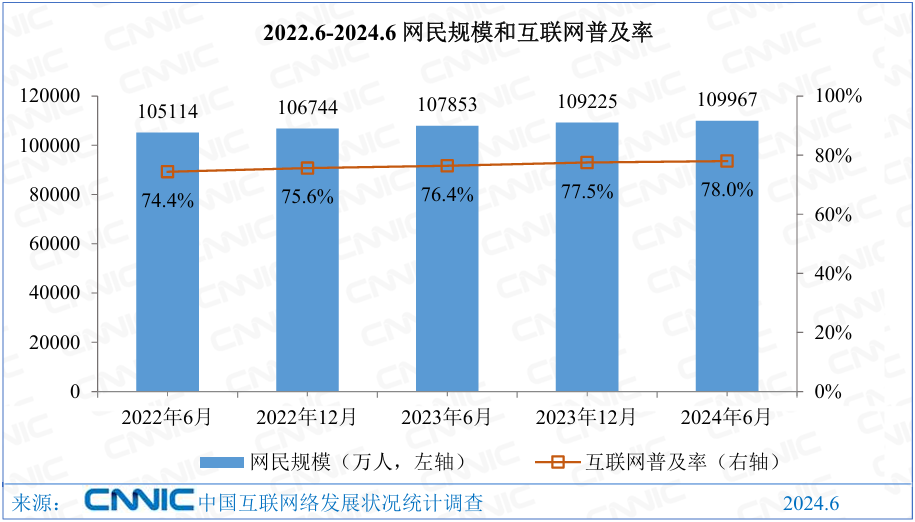
\includegraphics[width=1\linewidth]{./pic/网民规模.png}
    \caption{2022.6-2024.6 网民规模和互联网普及率\citing{CNNIC2024}}
    \label{netPeople}
\end{figure}

然而,随着互联网的蓬勃发展,网络安全形势日益严峻,网络攻击手段愈加复杂和多样,《中国网络安全产业分析报告(2024年)》\citing{ChinaCIA2024}中指出,2023 年以来,网络攻击活动呈现组织化程度高、攻击目标明确、攻击数量增多、隐蔽性增强、攻击效率提高等趋势,高级持续性威胁(Advanced Persistent Threat,APT)攻击、勒索软件攻击、数据窃取、零日攻击等网络攻击手段近年来已演化为结合社会工程学攻击、应用人工智能等前沿技术的综合体,网络空间安全威胁越来越严峻。据Statista网站统计显示\citing{statista_ransomware},全球72\%的企业成为勒索攻击受害者。2023年发生多起严重的网络攻击事件,例如,美国IvantiVPN设备零日漏洞受到攻击、美国医疗处方公司ChangeHealthcare 遭受网络攻击、XZUtils软件供应链攻击及7·19微软蓝屏事件造成全球近千万台设备宕机等,极大地暴露了网络安全防护的薄弱环节。

此外,随着互联网的快速发展,网络流量急剧增加,网络攻击的规模和手段也不断演变。恶意流量与正常流量存在显著差异,通常包含具有破坏性的行为,对网络安全构成严重威胁。因此,如何及时准确地检测和防范恶意网络流量成为保障互联网健康发展的关键。网络恶意流量检测技术在入侵检测领域中发挥着至关重要的作用,它通过分析关键网络节点收集的信息,实时识别潜在的威胁,从而确保网络的安全性、可用性以及数据的保密性与完整性。

在当前的恶意流量检测研究中,快速准确地识别恶意流量仍然是一个亟待解决的问题。尽管机器学习和人工智能技术在此领域已取得一定进展,仍面临流量数据处理、大规模数据适配、新型攻击检测以及网络环境适应性等挑战。为了克服这些难题,本研究提出了一种创新的恶意流量检测方案,结合了去噪扩散概率模型(Denoising Diffusion Probabilistic Model,DDPM)和图神经网络(Graph Neural Network,GNN)的方法。DDPM是一种生成模型,通过模拟数据在图像或其他数据空间中的扩散过程生成样本。在恶意流量检测中,DDPM可用于数据增强,生成多样化的训练样本,从而提高模型的泛化能力,帮助模型更好地适应新型攻击模式的识别。具体来说,DDPM通过噪声添加和去噪操作扩展了训练数据集,有效缓解了数据稀缺的问题,提升了模型对不同攻击的识别能力。另一方面,GNN通过在图结构上进行信息传递,能够捕捉节点间复杂的关系。在恶意流量检测中,网络流量可以看作是图结构数据,其中节点代表流量特征或网络设备,边代表它们之间的连接。GNN能够有效聚合邻域节点的信息,提取和传播网络流量中的复杂关系,从而增强对流量异常和恶意行为的检测能力。通过结合DDPM和GNN,本研究不仅能够扩充训练数据集,增强模型的泛化能力,还能利用GNN的图结构表示能力,更好地捕捉恶意流量中的复杂特征,从而提升恶意流量检测的准确性和鲁棒性。

基于图神经网络的恶意流量检测方法能够结合网络拓扑结构与流量特征,提升对复杂网络环境下恶意流量的检测能力。通过对网络流量的深度分析,本方法能够实时识别潜在的攻击行为,从而有效提高网络的安全性。因此,结合DDPM和图神经网络的方法,在恶意流量检测中展现出巨大的应用潜力,成为网络安全领域的重要研究方向。
\section{国内外研究现状}
网络恶意流量检测本质上是对流量进行分类,将其分为正常流量和恶意流量,而在现实情况下,流量的占比常常存在差异,尤其在分类任务中,这会导致数据不平衡问题,从而影响分类效果。因此,本节将围绕数据不平衡处理和恶意流量检测两个方面介绍国内外研究现状。 

\subsection{数据不平衡处理}


数据不平衡问题是机器学习中的一个重要课题,特别是当某一类别的样本数量明显少于其他类别时,传统机器学习模型通常会偏向于多数类,从而导致对少数类的识别效果显著降低。为了解决这一问题,研究人员提出了多种解决方案,包括数据采样、数据合成以及加权策略等。

数据采样应对不平衡数据,通过过采样增加少数类或欠采样减少多数类来调整类别比例,这种方法简单易行,但可能会丢失多数类样本中的重要信息。过采样增补少数类样本,确保原始信息不丢失,促进数据平衡,但也可能导致模型过拟合。为了克服这些缺点,研究者们提出了合成采样技术,如合成少数类过采样技术(Synthetic Minority Over-sampling Technique, SMOTE)。Chawla等人\citing{Chawla2002}提出的SMOTE技术通过在特征空间中生成合成的少数类样本,改善了少数类的分类性能,并在多个数据集上验证了其有效性。SMOTE通过在少数类样本的邻域内生成新合成样本,成功增加了少数类的样本数量,同时避免了单纯复制样本可能引发的过拟合问题。随后,Soltanzadeh\citing{Soltanzadeh2020}提出了一种改进的范围控制合成少数过采样技术(Range Controlled Synthetic Minority Over-sampling Technique, RCSMOTE),通过样本分类和改进的生成过程,有效避免了过采样中噪声样本的引入,同时减少了类别重叠。

生成对抗网络(Generative Adversarial Network,GAN)是一种强大的数据生成技术,能够创造出逼真的样本数据。GAN由两个部分构成:生成器和判别器,生成器负责样本的生成,而判别器则用于区分生成样本与真实样本。近年来,基于GAN的技术在处理不平衡数据集时取得了显著的成果,尤其是在生成少数类样本方面。Goodfellow等人\citing{Goodfellow2014}提出的生成对抗网络,通过对抗过程同时训练生成模型和判别模型,以生成高质量的样本数据,尤其在图像生成领域显示出了巨大潜力。Haloui等人\citing{Haloui2018}提出了基于Wasserstein生成对抗网络(Wasserstein Generative Adversarial Network, WGAN)的异常检测方法,用于时间序列数据集中的异常检测。该方法通过训练WGAN学习正常数据的分布表示,并结合编码器进行异常检测,从而提高了检测性能。Wu等人\citing{Wu2020}则提出了一种基于深度卷积生成对抗网络(Deep Convolutional Generative Adversarial Network, DCGAN)的数据增强方法,用于番茄叶片疾病识别。该方法通过生成逼真的叶片图像,扩充了数据集,提高了识别模型的泛化能力和准确性。Walter等人\citing{Walter2021}提出了渐进式生成对抗网络(Progressive Generative Adversarial Network, Progressive GAN)用于MIDI音乐生成,通过逐步增加网络复杂度和数据分辨率,提升了音乐生成的质量和稳定性。Yu等人\citing{Yu2023}则提出了一种改进的超分辨率生成对抗网络(Super-Resolution Generative Adversarial Network, SRDAGAN)应用于刨花板图像超分辨率重建,优化了网络结构和损失函数,从而有效提高了重建图像的质量和细节表现。

DDPM(Denoising Diffusion Probabilistic Models, DDPM)是另一种在生成高质量样本方面表现出色的数据合成技术。DDPM通过逐步去噪的过程生成样本,其生成效果在图像生成和音频生成等领域中常常超越GAN。DDPM的训练过程相对稳定,不容易出现模式崩溃等问题,且可用于数据增强,提高模型的泛化能力。最早由Ho等人\citing{ho2020denoising}提出,DDPM通过训练一个参数化的马尔可夫链,逆转逐步添加噪声的过程,从而生成符合数据分布的样本。Ding等人\citing{ding2021ccdm}提出了连续条件扩散模型(Continuous Conditional Diffusion Models, CCDM),在给定标量连续变量(回归标签)的条件下生成高维数据(如图像)。该模型通过改进的去噪U-Net架构和高效的条件采样程序,克服了现有条件扩散模型的局限性,显著提高了生成图像的质量。Jiang等人\citing{jiang2024fastddpm}提出了快速去噪扩散概率模型(Fast Denoising Diffusion Probabilistic Models, Fast-DDPM),旨在加速训练和采样过程。通过仅使用10个时间步,Fast-DDPM显著减少了训练和采样时间,在医学图像生成任务中表现出优于传统方法的性能。Lee等人\citing{lee2022priorgrad}则提出了PriorGrad方法,用于改进基于条件的去噪扩散模型,尤其是在语音合成领域。PriorGrad通过应用自适应先验,提高了模型的去噪效率,并在语音生成任务中显著提升了模型的感知质量和鲁棒性。

尽管在处理数据不平衡问题上取得了一些进展,但依然存在若干挑战。例如SMOTE及其变体对噪声敏感,可能产生异常特征的新样本。基于GAN的技术往往依赖于模型结构和超参数的选择,因此需要经过大量的实验和调整才能获得理想的效果。



\subsection{恶意流量检测}


随着网络技术的不断进步,网络安全问题变得愈加严重。恶意流量攻击,例如分布式拒绝服务(Distributed Denial of Service, DDoS)攻击、入侵行为、恶意扫描,已成为影响网络安全的主要威胁之一。为了有效检测和防御这些攻击,恶意流量检测技术得到了广泛的研究与应用。该方法主要依赖于规则匹配和统计特征分析,然而这些方法往往难以有效应对未知的或复杂的攻击。近年来,随着机器学习、深度学习和图神经网络(Graph Neural Network, GNN)等技术的不断发展,恶意流量检测技术逐渐向更加智能化、自动化的方向发展。

(1) 基于规则的恶意流量检测方法

基于规则的恶意流量检测方法依赖于人工构建的规则库,将恶意流量的特征定义为签名,匹配网络流量与规则库中的签名。当网络流量与规则匹配时,系统判定其为恶意流量。Kumar等人\citing{kumar2020integrated}提出一种基于规则的集成入侵检测系统(Intrusion Detection System, IDS),该系统在UNSW-NB15数据集和实时在线数据集(RTNITP18)上进行分析,能够检测网络中的五类攻击:Exploit、DOS、Probe、Generic和Normal。该系统通过分析UNSW-NB15数据集并设计了一个集成的分类模型,并且在实时数据集上进行了性能评估。评估结果表明,该模型相比于其他方法表现出更优的性能,包括更高的准确率、攻击检测率和较低的误报率。此外,该系统还能够检测包括正常流量在内的五类攻击,具有较低的误报率和较高的检测率,为网络入侵检测提供了一种有效的解决方案。

Zhang等人\citing{zhang2022realtime}提出一种基于关联规则库的实时建筑能源系统异常操作模式检测方法。该方法结合了专家系统和关联规则挖掘的优势,首先从历史操作数据中提取关联规则,建立异常和正常操作模式的规则库。然后,利用这些规则库对实时操作数据进行检测,以识别异常操作模式。该方法在实际的制冷机房中进行了应用和评估,结果表明能够成功检测出已知和未知的异常操作模式,提高了建筑能源系统的运行效率和节能效果。Yang等人\citing{yang2024follow}提出一种名为AnomalyRuler的基于规则的推理框架,用于视频异常检测。该框架利用大型语言模型(Large Language Models, LLMs),通过归纳和演绎两个阶段,从少量正常样本中总结规则,检测测试视频中的异常帧。在归纳阶段,LLM从少量正常参考样本中总结出正常模式的规则;在演绎阶段,根据这些规则识别测试视频中的异常帧。此外,该框架还设计了规则聚合、感知平滑和鲁棒推理策略以增强检测的鲁棒性。实验结果表明,AnomalyRuler在多个视频异常检测基准数据集上取得了优异的性能,展示了其在推理能力和领域适应性方面的优势。

Feng等人\citing{feng2017selecting}提出一种名为SCDFLOW的方法,用于在Android应用中选择关键数据流以检测异常行为。该方法通过分析恶意应用与良性应用在敏感数据流上的差异,选择关键数据流作为特征。SCDFLOW首先使用静态污点分析工具FLOWDROID提取应用中的敏感数据流,然后通过特征选择算法CFlowSel选择关键数据流。实验结果表明,SCDFLOW能够有效减少数据流特征的维度,并在MUDFLOW和DREBIN数据集上提高了恶意软件检测率,同时对内存消耗的影响可以忽略不计。该方法为基于异常数据流的恶意软件检测提供了一种有效的解决方案。

这种方法在已知攻击的情况下能够快速检测并响应,处理速度较快。规则库的构建和维护相对简单,且技术门槛较低,适用于简单的恶意流量模式检测。然而,这种方法主要依赖于已知攻击的特征,对于未知或变种攻击的检测能力有限。攻击者可以通过绕过规则库中的签名或修改攻击方式来规避检测。此外,随着攻击手段的不断变化,规则库需要持续更新,这对于维护团队来说是一个巨大的挑战。

(2) 基于统计特征分析的恶意流量检测方法

基于统计特征分析的检测方法通过分析网络流量的统计数据(如流量大小、协议字段分布等),运用统计学原理(如信息熵、概率理论等)来区分正常流量与异常流量。Liu等人\citing{liu2021}提出的波形统计方法,通过将数据包交换过程中的帧长信息转换为波形特征,从中提取关键的统计特性进行分类。该方法具有较好的实时性和较低的计算复杂度,但由于攻击者可以模仿正常流量的统计特性,因此容易发生误报或漏报,尤其是在面临新型或变种攻击时。

Thakkar\citing{thakkar2023}提出一种基于统计重要性融合的特征选择方法,用于深度神经网络(Deep Neural Networks, DNN)基础的IDS。该方法通过计算特征的标准差、均值与中位数的差异来评估特征的重要性,并根据这些统计量的融合结果对特征进行排序和选择,旨在提取出具有高可辨识度和偏差的相关特征,从而提高DNN-IDS在NSL-KDD、UNSW\_NB-15和CIC-IDS-2017等数据集上的性能,包括准确率、精确率、召回率、F1分数和误报率等指标。

Liu等人\citing{liu2021}提出一种基于粒子群优化(Particle Swarm Optimization, PSO)的入侵检测模型,用于物联网(Internet of Things, IoT)环境中的安全防护。该模型首先利用PSO-LightGBM算法对数据进行特征提取和降维,通过PSO优化LightGBM的参数来实现数据的双维度约简和特征提取,以解决大规模数据集的不平衡分布问题。然后将处理后的特征数据输入单类支持向量机(One-Class Support Vector Machine, OCSVM)进行建模,以检测和识别正常数据以及各种异常数据,包括低频攻击数据如后门、Shellcode和蠕虫等。实验结果表明,该模型在准确性、检测率、误报率和时间成本等方面均优于其他入侵检测技术,具有在实时IoT环境中部署的潜力。

Zhang等人\citing{zhang2021}提出一种多维特征融合和堆叠集成机制(Multidimensional Feature Fusion and Stacked Ensemble Mechanism, MFFSEM),用于网络入侵检测。该方法首先根据网络流量数据的特性,如时间、空间和负载等维度,提取多个基本特征数据集。然后,考虑这些基本特征数据集之间的关联和相关性,通过排列组合的方式构建多个综合特征数据集,以满足现实世界异常行为检测的需求。接着,在多个综合特征数据集上应用堆叠集成学习策略,训练多个基本分类器,并将它们的预测概率作为元分类器的输入,从而实现多维全局异常检测模型。实验结果表明,MFFSEM在KDD Cup 99、NSL-KDD、UNSW-NB15和CIC-IDS2017等数据集上的检测性能显著优于基本分类器和元分类器,以及其他知名的集成方法,具有较高的准确率、召回率、精确率和F1分数等指标。

基于统计特征方法计算开销相对较小,能够快速处理大规模网络流量,适合实时监控,并能够处理大部分常见的网络攻击,尤其是在网络行为相对稳定的情况下。然而,攻击者可以通过伪造正常流量的统计特征来绕过检测。对于高级攻击,尤其是那些隐蔽性强或变种频繁的攻击,基于统计特征的方法往往无法有效捕捉到其中的细节。同时,网络波动或正常流量出现异常时,可能会导致误报,从而降低检测系统的鲁棒性。

(3) 基于机器学习的恶意流量检测方法  

   基于机器学习的检测方法能够自动从网络流量数据中提取特征,利用机器学习模型(如支持向量机(Support Vector Machine, SVM)、决策树、随机森林)等进行分类。Salman等人\citing{salman2022machine}提出一种基于机器学习的框架,用于物联网设备识别和异常流量检测。该框架旨在应对IoT设备的异构性、资源限制和大规模部署带来的安全挑战。框架在网络边缘提取网络流的特征,包括数据包方向、大小、时间戳和传输协议等,以识别设备类型、流量类型,并检测网络攻击。通过比较不同的机器学习算法,发现随机森林在设备类型识别、流量类型分类和异常流量检测方面表现最佳,分别达到了94.5\%、93.5\%和97\%的准确率。该框架具有实时性和低开销的特点,能够在不进行数据包内容检查的情况下,仅通过统计特征实现对IoT流量的准确分类和异常检测。Waskle等人\citing{waskle2020intrusion}提出一种结合主成分分析(Principal Component Analysis, PCA)和随机森林算法的IDS。该系统旨在提高入侵检测的准确性和效率。首先,通过PCA对数据集进行降维处理,以减少数据的维度并提取主要特征,从而提高数据集的质量和处理效率。PCA通过计算数据集的协方差矩阵和特征向量,将高维数据转换为低维的主成分,保留了数据的主要信息。随后,采用随机森林算法进行分类。随机森林是一种集成学习方法,通过构建多个决策树并结合它们的预测结果,从而提升分类的准确性和鲁棒性。在实验中,该方法在KDD数据集上进行了测试,结果显示其性能优于传统的支持向量机(SVM)、朴素贝叶斯(Naive Bayes, NB)和决策树(DT)等方法。具体而言,该方法的性能时间为3.24分钟,准确率达到96.78\%,错误率仅为0.21\%。这表明该系统在检测网络入侵方面具有较高的准确性和较低的误报率,能够有效地识别和防御各种网络攻击。
   
相比于传统方法,机器学习能够自动从数据中学习到有用的特征,避免了人工特征选择的繁琐,具有较强的适应性,能够对未知的攻击类型进行有效学习。此外,机器学习方法可以结合多种算法进行集成学习,进一步提升分类效果。然而,在流量数据存在较大不平衡时,模型可能偏向于多数类,导致少数类的识别能力下降。机器学习模型通常需要大量的标注数据进行训练,对于恶意流量标注的获取和质量控制是一个挑战。与传统方法相比,机器学习模型的训练过程较为耗时,且对计算资源的需求较高。

(4) 基于深度学习的恶意流量检测方法  

   深度学习方法能够自动从原始数据中提取复杂的特征表示,适用于处理时序性强的流量数据,尤其是在面对动态网络流量时具有明显优势。Fu等人\citing{fu2022deep}提出一种基于深度学习的网络入侵检测模型(Deep Learning-based Network Intrusion Detection, DLNID),该模型旨在解决网络流量数据不平衡和检测准确率低的问题。模型结合了注意力机制(Attention Mechanism)和双向长短期记忆(Bidirectional Long Short-Term Memory, Bi-LSTM)网络,首先通过卷积神经网络(Convolutional Neural Network, CNN)首先提取数据流量的序列特征,然后通过注意力机制对每个通道的权重进行重新分配,以突出重要特征,最后使用Bi-LSTM学习序列特征之间的关系,从而提高入侵检测的准确率和F1分数。在NSL-KDD数据集上的实验结果表明,该模型的准确率和F1分数分别达到了90.73\%和89.65\%,优于其他比较方法。

Sinha\citing{sinha2020efficient}提出一种高效的深度CNN-BiLSTM模型,用于网络入侵检测。该模型充分利用了卷积神经网络(CNN)在学习数据空间特征方面的优势,以及双向长短期记忆(Bi-LSTM)在捕捉时间序列数据长期时间特征方面的能力。模型通过结合这两种网络结构,能够更准确地识别网络流量中的异常行为,提高检测率和降低误报率。实验在NSL-KDD和UNSW-NB15数据集上进行,结果表明该模型在二元分类和多类分类任务中均表现出色,高检测率伴以低误报率,优于许多现有的网络入侵检测系统。

Ge等人\citing{ge2021towards}提出一种基于深度学习的入侵检测方法,专门针对物联网环境中的网络安全问题。该方法采用定制的深度学习技术,利用包含IoT流量和真实攻击流量的先进IoT数据集,构建了一个前馈神经网络(Feedforward Neural Network, FNN)模型,并引入嵌入层来处理高维分类特征,实现对DoS、DDoS、数据收集和数据盗窃等攻击类型的多类分类。此外,该方法还应用迁移学习概念,将从多类分类模型中学习到的高维分类特征编码应用于二元分类器的构建,以进一步提高分类性能。实验结果表明,该方法在二元和多类分类任务中均取得了较高的分类准确率,分别为99.99\%和99.79\%,显示出良好的入侵检测性能。

深度学习能够自动从原始流量数据中提取关键特征,减少了人工特征工程的依赖,能够捕捉流量数据中的复杂模式和深层次关系,适应新型攻击模式。对于时序性强、长时间依赖关系明显的数据(如网络流量),深度学习能够更好地捕捉数据的动态特性。然而,深度学习模型训练需要大量的计算资源,且训练过程耗时较长,这在一些资源受限的环境中可能不可行。此外,深度学习模型的解释性较差,缺乏透明度,难以追踪决策过程,这可能在实际部署时带来一定的不确定性。深度学习模型也需要大量的标注数据,对于数据质量和数据集的多样性要求较高。

(5) 基于图神经网络的恶意流量检测方法  

图神经网络作为一种新兴的深度学习技术,能够处理图结构的数据。通过建模网络流量中的节点(如IP地址、端口等)及其之间的连接关系,图神经网络能够有效捕捉复杂的流量模式,提升检测的准确性。

Liu等人\citing{liu2020gnnad}提出了一种基于图神经网络的工控网络异常检测算法,旨在提高对联合异常攻击和恶意软件的检测能力。算法初始步骤是收集网络节点的状态,涉及相邻节点特征及它们的交互信息,通过该过程融合自身与邻近节点特征,以创建节点的新表示形式。然后,利用不动点理论对网络进行迭代更新,以求解每个节点状态向量的唯一解。接着,结合节点本身的特征与其邻域节点的特征,通过神经网络抽取更深层次的特征,从而生成节点的表示。最后,采用K-means聚类方法对节点特征进行聚类,判断网络节点是否是异常节点。实验结果表明,该算法在保持较高检测率的同时,也具有较高的鲁棒性,能够有效应对工控网络中的多点连接性,弥补了以往单点网络异常检测方法的不足。

Wang等人\citing{wang2025dgn}提出了一种基于深度强化学习的种子选择方法,用于解决社交网络中的影响力最大化问题。该方法构建了一个端到端训练的双耦合图神经网络,结合了深度学习的表示能力和强化学习的决策能力。具体来说,深度强化学习图神经网络(DGN)利用双耦合图神经网络对节点进行嵌入,捕捉社交网络的拓扑结构和节点属性信息,生成丰富的节点向量表示。同时,采用深度Q网络(Deep Q-Network, DQN)来探索社交网络的拓扑和节点属性信息,通过学习Q函数来近似当前状态和动作下的最优策略,从而自适应地选择种子节点,最大化影响力传播。实验结果表明,DGN在合成网络和真实网络上的性能接近或超越了当前最先进的模型,如ToupleGDD,并且在大规模、复杂和密集的社交网络中具有更好的鲁棒性。

Xu等人\citing{xu2024hcgae}提出了一种基于层次聚类的图自编码器(HC-GAE),用于图表示学习。HC-GAE在编码过程中,首先利用硬节点分配将样本图分解为多个分离的子图,然后对每个子图进行图卷积操作以进一步提取节点特征,并将属于每个子图的节点压缩成粗化节点,从而将原始图转换为粗化图。由于分离的子图之间没有连接,卷积操作无法在不同子图之间传播节点信息,从而显著减少了经典基于卷积的图自编码器中出现的过平滑问题。在解码过程中,采用软节点分配来重构原始图结构,通过扩展粗化节点。通过在解码过程中层次化地执行压缩过程以及在解码过程中执行扩展过程,HC-GAE能够有效提取原始样本图的双向层次结构特征,生成有效的图表示用于节点分类或图分类。此外,文章还重新设计了损失函数,整合了来自编码器和解码器的信息,以平衡训练过程中的局部和全局信息,进一步提升模型的表达能力。

Busch等人\citing{busch2021nfgnn}提出了一种基于网络流图的恶意软件检测和分类方法,利用图神经网络模型来分析网络流量数据。该方法首先从网络流量中提取流图,其中节点对应于网络中的端点,边表示端点之间的通信。与传统的将网络流视为独立实体的方法不同,该方法通过构建流图来捕捉网络中丰富的通信模式。文章介绍了三种模型变体,分别用于监督学习和无监督学习设置下的恶意软件检测和分类。监督学习模型(Network Flow Graph Neural Network Classification, NF-GNN-CLF)通过在表示学习模块后添加池化层和预测层来实现图分类,无监督学习模型包括图自编码器(Network Flow Graph Neural Network Autoencoder, NF-GNN-AE)和单类图神经网络(Network Flow Graph Neural Network One-Class, NF-GNN-OC),分别通过重建损失和单类损失来进行异常检测。实验结果表明,该方法在不同的预测任务中均优于现有方法,能够显著提高检测性能。该方法不仅能够处理标记数据,还能在无标记数据和少量训练数据的情况下取得良好的性能,展示了其在恶意软件检测领域的潜力。

Zhao等人\citing{zhao2020tgcn}提出了一种时间图卷积网络(T-GCN)模型,用于交通预测。T-GCN模型结合了图卷积网络(Graph Convolutional Network, GCN)和门控循环单元(Gated Recurrent Unit, GRU),以同时抓取时间以及空间依赖性。具体来说,空间维度上,GCN构建路网节点的拓扑表征;时间维度上,GRU建立观测值的动态关联,形成时空双重建模框架,GCN与GRU构成互补:前者处理非欧空间数据结构,后者建模序列数据的时变特性T-GCN模型首先将历史交通信息作为输入,通过GCN获取道路网络的空间特征,接着,将时空特征序列送入GRU,利用单元间信息流动捕捉时间序列特性。最终,通过全连接层输出预测值。实验结果表明,T-GCN模型在不同预测时间范围内的预测性能优于现有的最先进基线方法,如历史平均模型(Historical Average, HA)、自回归积分滑动平均模型(Autoregressive Integrated Moving Average, ARIMA)、支持向量回归模型(Support Vector Regression, SVR)、单独的GCN模型和GRU模型。此外,T-GCN模型在面对数据噪声时表现出良好的鲁棒性,能够处理高噪声问题,适用于短期和长期交通预测任务。



\section{本文的主要贡献与创新}


本文针对物联网恶意流量检测中存在的模型鲁棒性问题,提出了一种高鲁棒性的恶意流量检测方法。该方法的核心创新在于结合去噪扩散概率模型与图神经网络技术,旨在提升模型在不平衡数据环境下的识别能力,并增强模型在面对各种复杂网络流量时的适应性和稳定性。具体设计过程中,本文提出了两项关键技术:基于非功能性特征和低度 IP 的去噪扩散概率模型,以及基于线图的恶意流量检测方法。两者相互配合,有效地提升了恶意流量检测的准确性、鲁棒性和泛化能力。
全文结构如图\ref{fig:full-process}所示。
\begin{figure}[h!]
    \centering
    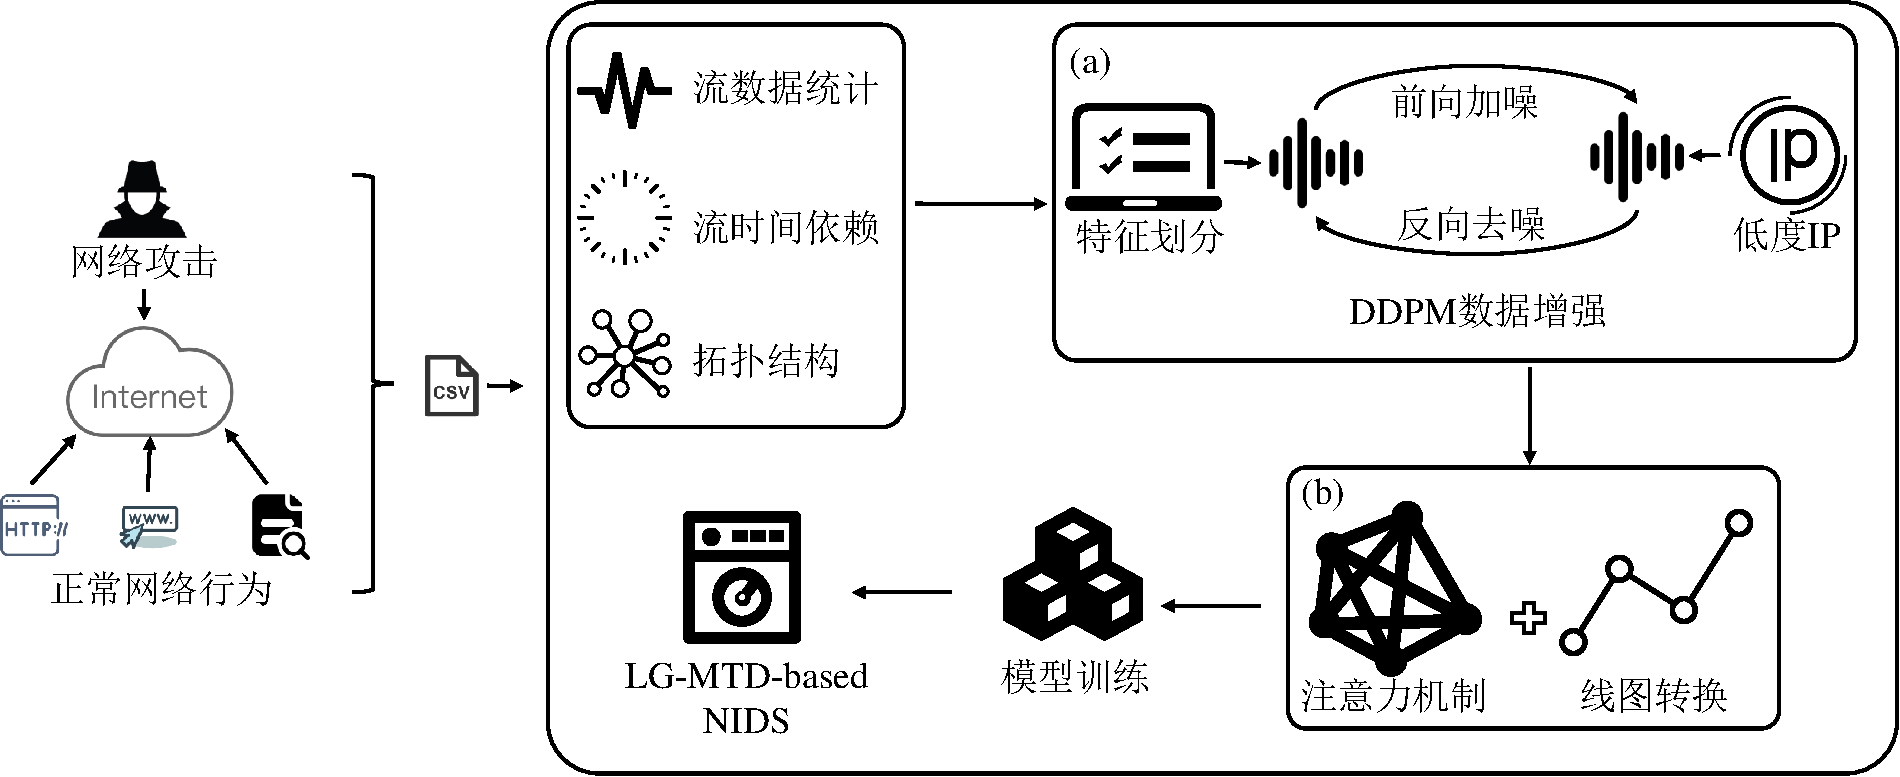
\includegraphics[width=1\linewidth]{./pic/full-process.pdf}
    \caption{全文结构图}
    \label{fig:full-process}
\end{figure}

(1) 基于非功能性特征和低度 IP 的去噪扩散概率模型  

   为了解决网络流量数据中的不平衡问题,尤其是低度 IP 的识别难题,本文提出了去噪扩散概率模型。如图\ref{fig:full-process}(a)所示。首先,采用清洗、标签转换和标准化的方式确保数据质量,并通过正则表达式提取功能性和非功能性特征,处理低度 IP 数据。通过结合功能性和非功能性特征的分类处理,模型能够有针对性地优化特征的权重分配和特征交互,从而提升低度 IP 流量的识别能力。进一步地,为提升模型的表现,本文引入了时序图结构来捕捉数据中的时间依赖性,并增强了模型的上下文感知能力。同时,结合低度 IP 掩码和数据增强技术,模型通过添加噪声并逐步去噪生成符合真实分布的样本,从而扩充了训练集并提升了模型的鲁棒性。

(2) 基于线图的恶意流量检测方法  

   为了进一步提升模型的表现,本文提出了一种基于线图的恶意流量检测方法。如图\ref{fig:full-process}(b)所示。首先,利用前述去噪扩散概率模型对训练数据进行增强,并采用线图结构来更有效地捕捉边的特征,从而提升模型的表达能力。接着,结合自适应多头注意力机制,动态调整节点之间的注意力权重,实现更精确的消息传递和特征聚合。这一机制帮助模型更好地捕捉节点间的复杂关系,增强了整体表现能力。最后,本文使用中位数绝对偏差(Median Absolute Deviation,MAD)指标来评估图神经网络在不同层次上的特征分布变化,特别是邻居节点与远程节点之间的特征差异。MAD指标有助于衡量特征分布的稳定性,减少异常值的影响,并提供了一种更为鲁棒的评估方式。通过这种方法,能够更好地理解图神经网络在流量数据中的特征差异性,进一步提升模型对流量数据的适应性和泛化能力,为图神经网络在流量数据中的应用提供新的分析视角。
\section{本论文的结构安排}
围绕上述研究内容,本文各章节内容安排如下:

第一章为绪论。首先阐述研究的背景及重要性,接着回顾恶意流量监测与流量分布不均处理在国内外的研究进展,最后概述本文的核心研究主题及文章结构。

第二章为相关理论及技术介绍,主要涵盖了以下几个方面的基础理论与技术:半监督学习、去噪扩散模型、恶意网络流量分析、神经网络及其原理、以及所使用的注意力机制。通过对这些理论和技术的介绍,为后续的研究方法与模型设计提供理论支持和技术框架。

第三章聚焦于LDNFDDPM在数据增强中的应用。本章首先评析生成对抗网络数据增强的局限,随后引出DDPM为基础的数据增强策略;
接着,详细叙述了从数据预处理到构建时序图,再到利用LDNFDDPM生成恶意流量数据的具体步骤。在三个数据集上验证了该方法具有良好的数据增强效果。

第四章为基于线图的恶意流量检测方法。首先介绍了传统图神经网络的不足和问题,然后详细阐述了如何利用线图来重构图,从而更好地捕捉边缘特征,接着描述了利用多头注意力机制来进
行图卷积操作以及利用半监督学习方法进行模型训练。在公开流量数据集上验证了该方法的恶意流量检测能力。


第五章为总结与展望。总结了本文的工作内容,并对下一步改进工作进行了展望。

\chapter{相关理论及技术介绍}
\section{恶意网络流量}
本部分探讨恶意网络流量的定义及典型网络攻击类型。恶意流量指的是意图不轨的数据传输,涉及如网络侵袭、恶意软件散布和钓鱼攻击等活动,与正常的、遵循协议的通信相对。识别这类流量对于维护网络安全和确保数据安全至关重要,因为攻击方式广泛,包括但不限于几种典型的网络攻击:

DDoS(分布式拒绝服务攻击)\citing{mirkovic2004taxonomy}利用全球分布的受感染计算机(常称僵尸网络)向目标发起海量请求,导致目标服务器资源耗尽,无法正常运行。通过分布式源发起,DDoS攻击难以追踪和防御,常常造成网站、服务器或网络基础设施的停机或服务不可用。

DoS(拒绝服务攻击)\citing{carl2006denial}是一种通过发送大量无效请求,导致目标系统资源耗尽,使得合法用户无法访问目标服务的攻击。通常由单一源发起,攻击者通过消耗系统资源(如内存、带宽、CPU等)使目标无法处理请求,造成系统崩溃或长时间不可用。

Backdoor(后门攻击)\citing{gao2020backdoor}指攻击者通过某种手段在目标系统中植入隐藏的入口(“后门”),从而绕过正常的认证机制,随时访问目标系统。通过恶意软件(如病毒、木马等)创建的后门,攻击者可以在系统内外随时控制受害设备,窃取敏感信息或执行恶意操作。

Injection(注入攻击)\citing{alghawazi2022detection}是指攻击者将恶意代码(如SQL代码、脚本等)插入到输入字段、请求参数或URL中,通过漏洞让目标系统执行恶意命令。注入攻击,如SQL注入、命令注入及XSS,常用来盗取数据、控制系统和干扰网络服务。

Password(密码攻击)\citing{wang2021attacks}是指攻击者通过破解目标用户的密码,获取非法访问权限的攻击方式。暴力破解、字典攻击和社交工程攻击是常见的密码攻击方法。成功的密码攻击可能导致系统或账户的控制权被窃取,进而造成数据泄露或系统滥用。

Scanning(扫描攻击)\citing{lee2003detection}是攻击者利用扫描工具探测目标系统的开放端口、服务或漏洞,寻找潜在的攻击入口。通过端口扫描和漏洞扫描,攻击者可以识别目标系统的弱点,为后续攻击提供依据。

XSS(跨站脚本攻击)\citing{gupta2017cross}是攻击者向网站注入恶意脚本,使得用户在访问网站时执行这些脚本,从而泄露敏感信息(如Cookie、凭证等)或执行其他恶意操作。XSS攻击包括存储型XSS和反射型XSS,分别通过存储在服务器上的脚本和通过URL传递的脚本来实现。

Theft(窃取攻击)\citing{leevy2021detecting}指攻击者利用非法手段窃取用户的敏感信息,包括用户名、密码、信用卡详情和机密文档。数据窃取和身份盗窃是窃取攻击的常见形式,攻击者通过盗用信息进行非法活动,给受害者带来金融损失或法律问题。

Reconnaissance(侦察攻击)\citing{jafarian2015effective}是攻击者在实际发起攻击之前,对目标系统和网络进行调查和侦察,以收集尽可能多的信息。攻击者可能通过社交工程、网络嗅探和域名查询等手段收集有关目标的信息,并通过网络映射来识别系统架构、端口、设备等,为后续攻击提供基础。

Brute Force(暴力破解攻击)\citing{knudsen2011block}是一种通过反复猜测用户名和密码组合来获取系统访问权限的攻击方式。攻击者通过尝试尽可能多的密码组合,直到找到正确的密码。暴力破解常用于破解简单的密码或账号,如果目标密码较弱,攻击者可能轻易获得访问权限。

\section{去噪扩散模型}
本节主要介绍去噪扩散模型。去噪扩散模型最初由Ho等人\citing{ho2020denoising}提出,旨在解决图像生成问题。其通过逐步添加噪声来训练模型,并通过逐步去噪的过程生成数据。近年来,DDPM成功应用于恶意流量检测和数据增强领域。Gong等人\citing{gong2025network}提出了一种自适应常微分方程求解器变换器网络扩散模型(Adaptive ODE Solver Transformer Network Diffusion Model,AOT-DDPM)的网络流量数据生成模型,用于异常流量检测。该模型结合了自适应采样策略、Transformer网络结构和ODE求解器,有效解决了网络流量数据不平衡的问题,并显著提高了异常流量检测的准确率和效率。

在恶意流量检测中,DDPM的应用场景包括通过增强数据集来改善模型对低频异常流量的识别能力。由于网络流量数据中通常存在大量的正常流量和少量的恶意流量,导致数据不平衡问题。DDPM通过生成与真实流量分布相似的虚拟流量数据,扩充训练集,帮助模型更好地学习和识别恶意流量的特征。此外,DDPM的逐步去噪过程能够保留流量数据的细节信息,有助于模型在处理复杂、动态变化的网络环境时保持较高的鲁棒性和泛化能力。这使得DDPM在恶意流量检测任务中,尤其是面对数据不平衡和高维度复杂特征时,具有显著的优势。

DDPM是一类基于扩散过程的生成模型,其核心思想是通过一个渐进的过程,将数据从清晰的状态变为噪声,然后通过反向过程逐步去噪,恢复出原始数据。


正向扩散过程的目标是将原始数据样本 \( x_0 \) 逐步加入噪声,直至将其转变为噪声。这个过程是一个马尔科夫链,可以通过以下公式描述:
\begin{equation}
q(x_t | x_{t-1}) = \mathcal{N}(x_t; \sqrt{1 - \beta_t} x_{t-1}, \beta_t \mathbf{I})
\end{equation}
其中,\( \mathcal{N} \) 表示高斯分布,\( \beta_t \) 是每个时间步的噪声调度参数,控制每一步加入的噪声强度。通过递归计算,可以得到每个时间步的样本:
\begin{equation}
x_t = \sqrt{1 - \beta_t} x_{t-1} + \sqrt{\beta_t} \epsilon_t
\end{equation}

其中 \( \epsilon_t \sim \mathcal{N}(0, \mathbf{I}) \) 是均值为 0,方差为 1 的高斯噪声。

最终,正向过程会将原始样本 \( x_0 \) 转变为标准正态分布 \( x_T \),即:
\begin{equation}
q(x_t | x_0) = \mathcal{N}(x_t; \sqrt{\bar{\alpha_t}} x_0, (1 - \bar{\alpha_t}) \mathbf{I})
\end{equation}

其中,\( \alpha_t = 1 - \beta_t \) 且 \( \bar{\alpha_t} = \prod_{s=1}^t \alpha_s \)。



在反向扩散过程中,通过训练一个神经网络 \( p_{\theta}(x_{t-1} | x_t) \) 来近似学习如何从噪声中恢复原始数据。反向过程的公式为:
\begin{equation}
p_{\theta}(x_{t-1} | x_t) = \mathcal{N}(x_{t-1}; \mu_{\theta}(x_t, t), \Sigma_t)
\end{equation}

其中,\( \mu_{\theta}(x_t, t) \) 是由神经网络预测的去噪值,\( \Sigma_t \) 是噪声方差(通常为常数或学习得到的调度)。



DDPM的训练目标是最大化数据的对数似然 \( \log p_{\theta}(x_0) \),即最小化正向过程和反向过程之间的KL散度。训练中的损失函数通常表示为去噪误差,公式为:
\begin{equation}
\mathcal{L}_{\text{DDPM}} = \mathbb{E}_{q(x_0, x_1, \dots, x_T)} \left[ \sum_{t=1}^{T} \left\| \mathbf{\epsilon}_\theta(x_t, t) - \mathbf{\epsilon} \right\|^2 \right]
\end{equation}

其中,\( \mathbf{\epsilon}_\theta(x_t, t) \) 是网络预测的噪声,\( \mathbf{\epsilon} \) 是实际的噪声,\( T \) 是扩散过程的步数。



在生成过程中,从一个标准正态分布的噪声样本 \( x_T \sim \mathcal{N}(0, \mathbf{I}) \) 开始,通过反向扩散过程逐步去噪,生成样本。每一步的去噪操作可以表示为:
\begin{equation}
x_{t-1} = \mu_{\theta}(x_t, t) + \sigma_t \cdot \epsilon_t
\end{equation}

其中,\( \epsilon_t \sim \mathcal{N}(0, I) \) 是用于增加噪声的高斯噪声,\( \sigma_t \) 是标准差,控制噪声的强度。



\section{半监督学习}
本节主要介绍半监督学习。在许多实际机器学习应用中,容易获取大量的无标签数据,但要通过特殊设备或昂贵且耗时的实验过程才能标注数据,导致有标签数据稀缺。为了充分利用无标签数据,半监督学习\citing{learning2006semi}应运而生,如图\ref{halfSupervised}所示,它将大量的无标签样本与少量的有标签样本结合起来,进行训练,从而改善学习性能。
\begin{figure}[h!]
    \centering
    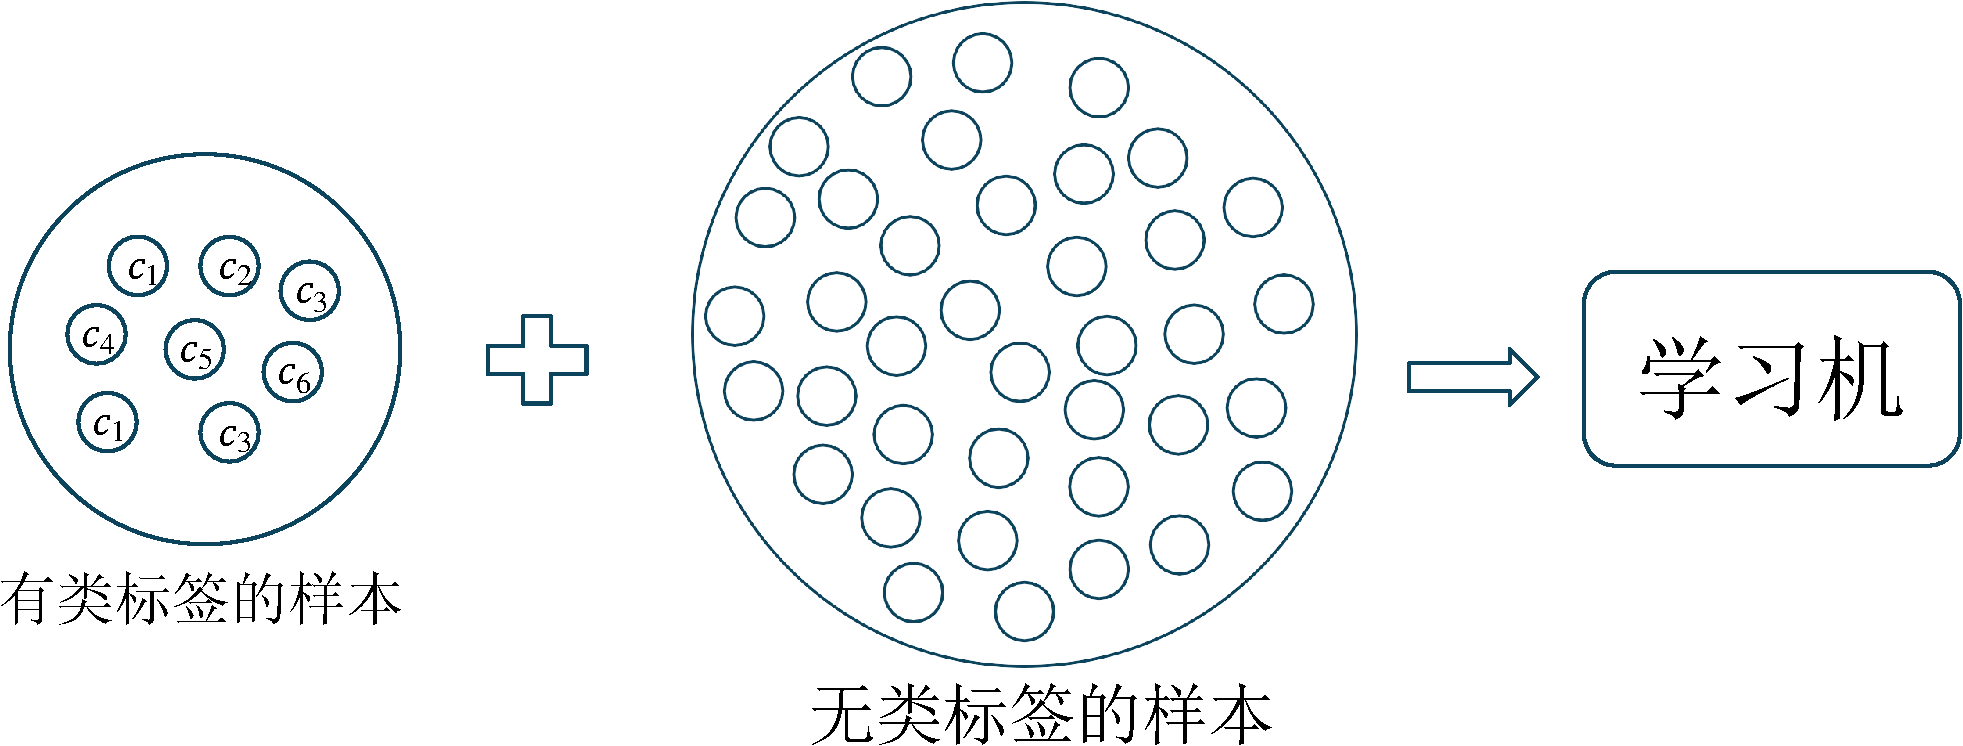
\includegraphics[width=1\linewidth]{./pic/semi-supervision.pdf}
    \caption{半监督学习}
    \label{halfSupervised}
\end{figure}

半监督学习的主要目标是减少资源消耗,半监督学习兼顾监督学习的泛化限制与无监督学习的精度挑战。其应用广泛,包括:

1. 无标签数据远多于有标签数据。

2. 直推半监督学习:直推半监督学习只考虑已知的训练数据,利用有标签数据和无标签数据进行训练,并预测无标签样本的标签。预测的目标是尽量让模型对训练集中的无标签数据进行准确预测。目标是提高模型的泛化能力,特别是在无标签数据的帮助下。
\begin{equation}
\hat{y} = f(x; \theta)
\end{equation}

其中,\( \hat{y} \) 是对样本 \( x \) 的预测,\( f(x; \theta) \) 是模型,\( \theta \) 是参数。

3. 归纳半监督学习:归纳半监督学习不仅利用已标记和未标记的样本,还处理整个样本空间,包括未标记的数据和测试数据。通过归纳半监督学习,模型不仅可以对无标签的训练样本进行预测,还能预测未知的测试样本的标签。
\begin{equation}
\mathcal{L}_{\text{inductive}} = \sum_{i=1}^{N} \mathcal{L}(y_i, f(x_i; \theta))
\end{equation}

其中,\( \mathcal{L} \) 是损失函数,\( y_i \) 是标签,\( f(x_i; \theta) \) 是模型预测。

在归纳半监督学习中,假设训练数据中的无标签样本并不直接对应测试数据,而是作为模型泛化能力提升的辅助数据。与此不同,直推半监督学习假设未标记的样本恰恰是需要关注的待预测数据。

通过这种方式,半监督学习擅长在有限的标注数据环境中,借助未标注数据来增强模型的表现和泛化水平。
\section{图神经网络}

本节主要介绍图神经网络\citing{gao2023survey}。GNN(图神经网络)是专为分析和学习图数据而设计的神经网络模型。图结构数据广泛存在于许多实际应用中,如社交网络、分子结构、知识图谱等。在这些图中,节点代表个体或物体,边则表示节点之间的关系。GNN的核心在于,它通过信息的传递与整合,来学习图中节点、边的高效表示,从而捕捉图中的复杂连接模式和高阶关联信息。

GNN的基本操作是基于节点邻域的消息传递。每个节点接收邻居节点的信息,并通过神经网络对接收到的信息进行聚合和变换,从而更新自身的特征表示。通过多层堆叠,信息会逐渐从局部传播到全局,最终使得每个节点的特征包含整个图的高阶信息。

GNN模型通常分为两大类:

谱模型(Spectral Models):通过图信号的谱变换(如图傅里叶变换)进行卷积操作,依赖于图的全局性质,计算复杂度较高。

空间模型(Spatial Models):直接在图结构上进行卷积操作,通过加权聚合邻居节点的信息来提取局部特征,计算效率较高,适用于大规模图数据。

GNN广泛应用于推荐、社交分析、分子特性预测和知识图谱等场景。相比传统的矩阵分解或浅层学习方法,GNN能够利用图结构中的高阶连接信息,捕捉节点之间的复杂关系,从而增强模型的表现力和鲁棒性。

\section{图卷积网络}

本节主要介绍图卷积网络(Graph Convolutional Network,GCN)\citing{gao2023survey},它是图神经网络中的一种重要模型,属于谱模型。GCN的核心思想是通过图傅里叶变换将图信号转换到谱域进行滤波,随后再将处理后的信号转换回空间域。GCN利用图的邻接矩阵和度矩阵来定义卷积操作,从而实现对图信号的平滑和特征提取。

GCN的卷积操作基于图的谱理论。通过对图信号进行傅里叶变换将其映射到谱域,随后在该领域应用滤波器执行卷积操作,最终通过逆变换返回至空间域。具体地,GCN通过以下公式对节点特征进行更新:
\begin{equation}
H^{(l+1)} = \sigma(\tilde{D}^{-\frac{1}{2}}\tilde{A}\tilde{D}^{-\frac{1}{2}}H^{(l)}W^{(l)})
\end{equation}

其中:
 \( H^{(l)} \) 是第 \( l \) 层的节点特征矩阵,表示每个节点的特征表示;
 \( \tilde{A} = A + I \) 是带自环的邻接矩阵,\( I \) 为单位矩阵;
 \( \tilde{D} \) 是度矩阵,\( \tilde{D}_{ii} = \sum_j \tilde{A}_{ij} \);
 \( W^{(l)} \) 是第 \( l \) 层的可学习权重矩阵;
 \( \sigma \) 是激活函数(如ReLU)。

GCN通过多层堆叠来进行特征聚合,随着层数的增加,节点的特征向量包含了更多来自邻居节点的信息,从而实现了信息的传播和聚合。

GCN在处理节点分类、图级分类和预测边的连接性方面尤为高效。例如,在推荐系统中,GCN通过学习用户与物品之间的图嵌入,捕捉用户与物品之间复杂的关系,提升了推荐系统的准确性和多样性。在社交网络中,GCN被用来分析社交关系和发现社区。在图像处理和计算机视觉中,GCN能够处理图像的结构信息,增强模型的表现力。

\section{图注意力机制}
本节主要介绍图注意力机制。图注意力机制(Graph Attention Mechanism,GAM)\citing{velivckovic2017graph}是一种针对图数据的处理方法,它通过为每个节点的邻居分配个性化权重来聚合信息,强化了对节点间复杂关系的捕获和结构特征的利用。该机制使节点能基于邻居特征自适应地调整表示,有效处理图中的结构信息,并且具备高效的并行处理能力,尤其适合处理节点度数各异的情况,并且不需要全局图结构信息,使得模型能够高效地处理大规模图数据。

对于每个节点 \(i\),首先对其邻居节点 \(j\) 的特征进行线性变换,然后通过共享的注意力机制 \(a\) 来计算注意力系数 \(e_{ij}\),表示节点 \(j\) 的特征对节点 \(i\) 的重要性。计算公式为:
\begin{equation}
    e_{ij} = a(W\vec{h}_i, W\vec{h}_j)
\end{equation}

其中,\( W \) 是权重矩阵,\( \vec{h}_i \) 和 \( \vec{h}_j \) 分别是节点 \(i\) 和 \(j\) 的特征向量。为了使不同节点的注意力系数可比较,模型使用 softmax 函数对注意力系数进行归一化,得到最终的注意力权重 \( \alpha_{ij} \):
\begin{equation}
    \alpha_{ij} = \text{softmax}_j(e_{ij}) = \frac{\exp(e_{ij})}{\sum_{k \in \mathcal{N}_i} \exp(e_{ik})}
\end{equation}

其中,\( \mathcal{N}_i \) 是节点 \(i\) 的邻居节点集合。利用归一化后的注意力权重,模型对邻居节点的特征进行加权求和,得到节点 \(i\) 的最终特征表示:
\begin{equation}
    \vec{h}'_i = \sigma\left( \sum_{j \in \mathcal{N}_i} \alpha_{ij} W\vec{h}_j \right)
\end{equation}

其中,\( \sigma \) 是非线性激活函数,用于引入非线性特性。

为了进一步提升模型的表达能力,图注意力机制通常采用多头注意力(multi-head attention)。具体来说,该模型结合多个独立注意力分支的输出,通过拼接或平均处理,生成每个节点的综合特征表示。例如,对于 \(K\) 个注意力头,节点 \(i\) 的最终特征表示为:
\begin{equation}
    \vec{h}'_i = \sigma\left( \frac{1}{K} \sum_{k=1}^{K} \sum_{j \in \mathcal{N}_i} \alpha^k_{ij} W^k \vec{h}_j \right)
\end{equation}

其中,\( \alpha^k_{ij} \) 和 \( W^k \) 分别是第 \(k\) 个注意力头的注意力权重和权重矩阵。

图注意力机制通过引入动态的邻居加权策略,使得每个节点能够根据邻居节点的特征来自动分配权重,提升了模型在图结构数据中的表达能力。它不仅能有效捕捉图的局部结构信息,还能在处理图数据时具有较高的计算效率,尤其适合处理大规模图数据。图注意力机制,尤其在图分类、节点区分和链接预测上展现高效性能,且能与其它GNN模型集成增强功能。

\section{本章小结}
本章概览了网络恶意流量及其分析技术,涵盖基础概念、攻击类型,并详细阐述了半监督学习、去噪扩散、图神经网络家族(包括图卷积网络和图注意力机制)的关键原理,重点介绍了在研究中应用的图注意力机制。
\chapter{基于LDNFDDPM的数据增强方法}
本章提出了一种基于非功能性特征和低度IP的去噪扩散概率模型(Low-Degree and Non-Functional Feature based Denoising Diffusion Probabilistic Model,LDNFDDPM),旨在解决流量数据不平衡问题。首先,对原始数据进行了清洗、标签转换和标准化,确保数据质量。然后,通过正则表达式提取功能性特征(如网络协议、端口、ICMP类型)和非功能性特征(如流量统计、主机信息)。对训练数据中的低度IP进行处理,并结合特征分类优化模型。
为了增强模型的表现,引入时序图,捕捉数据的时间依赖性,提供更丰富的上下文信息。将数据集划分为训练集和测试集。训练集经过功能性和非功能性特征划分,并生成低度IP掩码,以便进行数据增强。

该方法通过向数据中添加噪声并逐步去噪,生成符合真实分布的样本,从而扩充训练数据集并提高模型的鲁棒性。该模型不仅改善了低度IP的识别能力,还增强了整体模型的泛化能力。

\section{问题描述和研究思路}
恶意流量检测对网络安全至关重要,涉及实时分析以揪出潜在威胁。在物联网场景中,由于正常流量远多于罕见的恶意流量,且分散的IP更易受袭,造成了类别不平衡问题。这挑战了AI模型,易使其偏向学习正常流量特征,进而影响对恶意流量的识别能力,增加误判和漏检的风险。

去噪扩散概率模型是一种基于扩散过程的生成模型。它由Sohl-Dickstein等人\citing{ho2020denoising}在2015年首次提出,并在近年来成为生成模型领域的重要研究方向。DDPM的核心思想是在数据生成过程中引入噪声,并通过逐步去噪来恢复原始数据,从而进行有效的样本生成。DDPM广泛应用于图像生成、视频生成、语音生成等领域。近年来,DDPM在多个生成任务上取得了超越GAN和VAEs(变分自编码器)的表现。在图像生成领域,DDPM通过逐步去噪的方式能够生成质量非常高的样本,特别是在高分辨率图像生成上表现尤为突出。

DDPM在处理流量图数据时,虽然具备生成高质量样本的能力,但也存在一些局限性,尤其是在流量数据的特征复杂性和数据不平衡问题上。流量图数据通常包括多种类型的节点和边特征,这些类别特征的多样性和异质性使得DDPM在直接应用时面临挑战。特别是在流量图中的节点,如IP地址,可能会涉及到不同等级的IP,其中部分低度IP节点(即与其他节点连接较少的节点)在生成过程中常常被忽略。低度IP节点通常代表着稀有攻击类型的特征,但由于其在真实流量中出现的频率较低,传统DDPM模型可能无法有效学习到这些特征,从而影响生成模型对稀有攻击类型的生成能力。

此外,流量图中的特征通常分为功能性和非功能性特征两种类型。功能性特征包括协议类型、端口信息、ICMP类型等,反映了网络流量的基础结构和通信方式。而非功能性特征则包括流量统计信息、主机信息、时延等,主要描述了流量的性质和行为模式。DDPM在进行生成任务时,通常未针对这些不同类型的特征进行特殊处理,可能会对非功能性特征的噪声过度增强,进而导致生成数据的质量下降。

此外,传统的DDPM方法也没有充分考虑到数据的不平衡问题,特别是对于攻击类型之间的差异。攻击流量(如DDoS、Bruteforce等)相较于正常流量(如Benign)通常较少,这种数据不平衡会影响DDPM的学习效果,导致模型无法很好地生成较为罕见的攻击流量,从而影响生成数据的多样性和完整性。
\begin{figure}[h!]
    \centering
    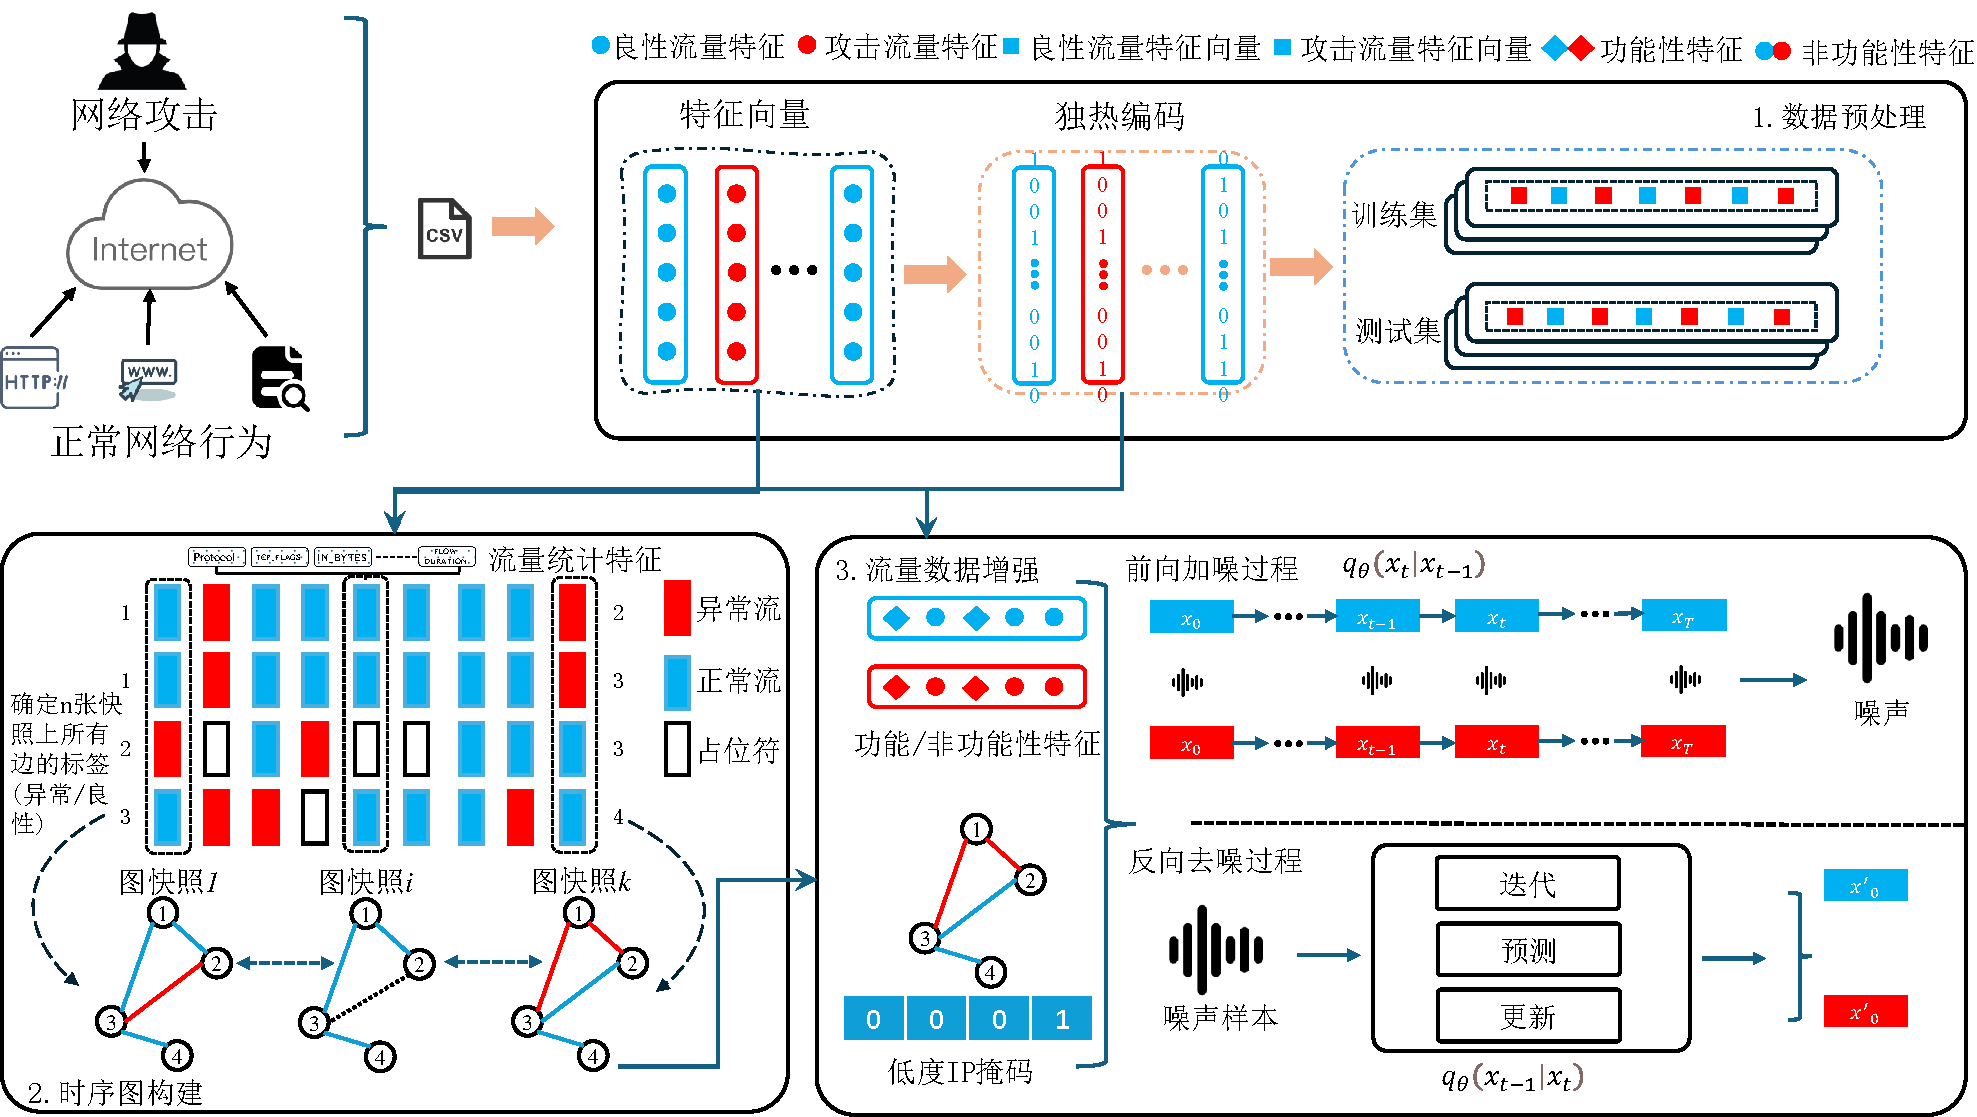
\includegraphics[width=1\linewidth]{./pic/框架图(大字版).pdf}
    \caption{基于 LDNFDDPM 的恶意流量数据增强}
    \label{frame}
\end{figure}

针对这些不足,本研究提出了一种改进的DDPM方法——基于低度IP与非功能性特征的DDPM(LDNFDDPM)。该方法在传统DDPM的基础上引入了低度IP节点的计算和功能性、非功能性特征的划分,以更好地处理流量图数据中的特征复杂性和不平衡问题。通过计算低度IP节点,并专门为其设计增强策略,LDNFDDPM能够有效地学习稀有攻击类型的特征,确保生成的流量样本包含了更多真实世界中可能遇到的攻击场景。同时,通过划分功能性和非功能性特征,并对其分别进行建模和处理,模型能够在生成过程中保留非功能性特征的重要信息,避免对这些特征的噪声过度增强,从而提高了生成数据的质量和多样性。

LDNFDDPM方法不仅解决了传统模型在处理流量图数据时的不足,还增强了模型对稀有事件、低度IP节点和多样化特征的捕捉能力,从而为网络流量检测和生成任务提供了更为准确和鲁棒的数据增强方案。


LDNFDDPM的总体结构如图\ref{frame}所示,包含三个主要模块:数据预处理模块、时序图构建模块和基于LDNFDDPM的恶意流量生成模块。

数据预处理模块:数据预处理模块是整个流程的第一步,主要包括特征工程和数据标准化。首先,原始流量数据需要进行清洗,处理缺失值和异常值,并对标签进行转换,确保数据的有效性。接着,特征选择和标准化步骤确保了不同特征的尺度一致,为后续的建模和训练提供了合适的输入。此外,任务集构造根据实验需求构建训练集和测试集,为后续模型的训练与验证奠定基础。

时序图构建模块:该模块将主机之间的时序关系抽象为时序图。在流量图中,每个主机(即IP节点)之间的通信可以视为图中的边,时序图的构建则关注通信的顺序和时延等信息。通过捕获流量图中节点之间的时序依赖关系,时序图构建模块能够有效地表达网络流量的动态特性,为后续流量生成和异常检测提供支持。

基于LDNFDDPM的恶意流量生成模块: 在时序图的基础上,LDNFDDPM恶意流量生成模块根据物联网流量数据集的不平衡性进行流量增强。首先,基于特征类型与作用,将原始物联网流量特征向量分为功能性和非功能性特征。功能性特征主要包括网络协议类型、端口号等,而非功能性特征则涵盖流量统计、主机信息等。其次,统计低度IP(即与其他节点连接较少的IP)并生成相应的掩码。低度IP通常与异常或攻击行为相关,因此对这些IP的关注有助于检测潜在的攻击流量。

最后,LDNFDDPM将非功能性特征和低度IP作为噪声关注点,结合去噪过程生成新的特征向量。此过程不仅提高了生成样本的多样性,还显著增强了流量生成的真实性,特别是在生成稀有攻击流量时。通过这一改进,LDNFDDPM能够有效应对数据不平衡问题,生成更加符合实际网络流量分布的恶意流量样本,从而提升模型的鲁棒性和准确性。
\section{框架设计}

\subsection{数据预处理}
数据预处理是恶意流量分类任务中的关键步骤。在实际的网络流量数据中,流量特征常常包含噪声、缺失值和冗余信息,这些问题若不加以处理,会影响模型训练的效果。因此,进行有效的数据预处理至关重要。本研究在数据预处理阶段,依照以下几个步骤进行操作,以确保数据质量和特征的有效性。具体的流程图如\ref{DataPreprocessing}所示。
\begin{figure}[h!]
    \centering
    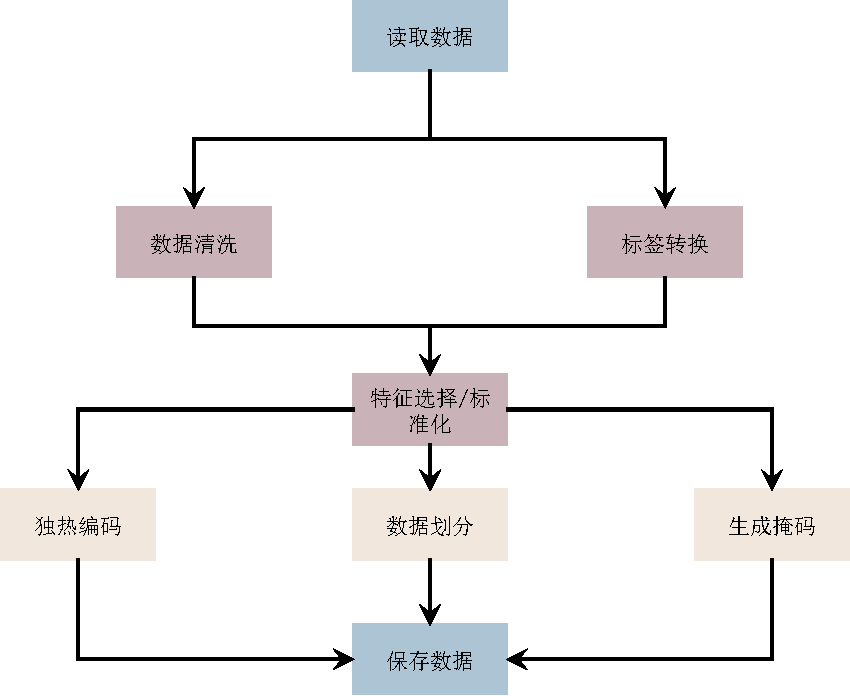
\includegraphics[width=0.75\linewidth]{./pic/数据预处理.pdf}
    \caption{数据预处理}
    \label{DataPreprocessing}
\end{figure}
为了让模型能够更好地进行训练,首先,对原始数据集进行清洗。由于流量数据的多样性,可能会存在缺失值和异常值,这些不完整或错误的数据会严重影响后续分析的准确性。因此,通过删除或填补缺失值、去除异常值等方法,确保数据集的完整性与准确性。

针对攻击类型标签,本研究对原始标签进行了转换。网络攻击类型包括:DoS(拒绝服务攻击)、DDoS(分布式拒绝服务攻击)、Reconnaissance(侦察攻击)、Theft(盗窃攻击)以及Benign(正常流量)。为了便于后续模型训练,通过标签编码的方式,将这些文本标签转换为数值型标签。具体来说,DoS标记为1,DDoS为2,Reconnaissance为3,Theft为4,正常流量为0。

\begin{table}[h!]
    \centering
    \caption{部分网络流量特征}
    \begin{tabular}{c||c}
     \hline \hline
        \textbf{特征} & \textbf{描述} \\ \hline
        \textbf{IN\_BYTES} & 输入流量字节数 \\  \hline
        \textbf{OUT\_BYTES} & 输出流量字节数 \\  \hline
        \textbf{FLOW\_DURATION\_MILLISECONDS} & 流持续时间 \\  \hline
        \textbf{DURATION\_IN} & 入站流持续时间\\  \hline
        \textbf{DURATION\_OUT} & 出站流持续时间 \\  \hline
        \textbf{MIN\_TTL} & 最小TTL(生存时间) \\  \hline
        \textbf{MAX\_TTL} & 最大TTL \\  \hline
        \textbf{LONGEST\_FLOW\_PKT} & 流最大数据包长度 \\  \hline
        \textbf{SHORTEST\_FLOW\_PKT} & 流最小数据包长度 \\  \hline
        \textbf{SRC\_TO\_DST\_SECOND\_BYTES} & 源到目标的第二级别字节数 \\  \hline
        \textbf{DST\_TO\_SRC\_SECOND\_BYTES} & 目标到源的第二级别字节数 \\  \hline
        \textbf{RETRANSMITTED\_IN\_BYTES} & 重新传输的入站字节数 \\  \hline
        \textbf{RETRANSMITTED\_OUT\_BYTES} & 重新传输的出站字节数 \\  \hline
        \textbf{SRC\_TO\_DST\_AVG\_THROUGHPUT} & 源到目标的平均吞吐量 \\  \hline
        \textbf{DST\_TO\_SRC\_AVG\_THROUGHPUT} & 目标到源的平均吞吐量 \\ \hline \hline
    \end{tabular}
    \label{tbl:network_features}
\end{table}
其次,针对特征选择,考虑到对模型训练的有效性,选择了62个特征,它们分别是流量特征:这些特征反映了流量的传输量,包括输入和输出的字节数和流量的二级单位字节数(如源到目标和目标到源的字节数)。包数特征:这类特征记录了网络通信中的包的数量,包括传输的包数以及重新传输的包数,这对于识别重复传输流量有很大帮助。流持续时间:表示网络连接持续的时间,能够帮助判断流量的持续性,尤其对DDoS类攻击的检测非常重要。时间相关特征:这些特征(如TTL值)有助于揭示数据包的生命周期和传输路径,特别是在网络攻击中,TTL值的变化常常反映异常行为。流量大小特征:涉及流量包的最大最小尺寸,有助于揭示攻击流量的异常模式,如流量包过大或过小。吞吐量特征:衡量源和目标之间的数据传输速率,突发流量和持续性攻击(如DDoS)通常在吞吐量上表现出异常特征。TCP窗口特征:TCP窗口大小影响数据流的传输速率,分析窗口大小的最大值可以揭示网络的流量控制机制,以及潜在的攻击行为。DNS特征:这些特征与DNS查询相关,能够揭示网络中的域名解析活动,有助于检测DNS放大攻击等特定类型的攻击。部分选取的特征如表\ref{tbl:network_features}所示。

进一步对这些特征进行处理,在流量数据分析中,许多类别特征如协议类型、端口号、标志位等通常是非数值型的,直接将其用于模型训练可能导致模型对特征关系产生误解。因此,必须将这些类别特征转化为数值特征,使得机器学习模型能够有效地进行训练。独热编码(One-Hot Encoding)是处理类别特征的常用方法,它将每个类别值转换为一个新的二元特征,确保模型不会误解类别之间的顺序或数值关系。在本研究中,对多种关键类别特征进行了独热编码,以便模型能够准确理解不同类别特征所代表的信息,提升模型在流量分类任务中的表现。

具体而言,研究中选择了包括 PROTOCOL(协议类型)、TCP\_FLAGS(TCP标志)、CLIENT\_TCP\_FLAGS(客户端TCP标志)、SERVER\_TCP\_FLAGS(服务器端TCP标志)、DNS\_QUERY\_TYPE(DNS查询类型)、FTP\_COMMAND\_R\\ET\_CODE(FTP命令返回代码)等类别特征进行独热编码。这些特征直接影响流量的网络行为模式,且在恶意流量检测中具有重要作用。例如,协议类型(如TCP、UDP、ICMP等)对流量的传输和攻击行为有重要指示作用,TCP标志和客户端/服务器端的TCP标志位反映了连接的状态信息,这些信息对流量分类尤其是恶意流量的识别至关重要。同样,DNS查询类型和FTP命令返回代码也常常用于表征特定的攻击行为模式,如DNS放大攻击或特定的网络扫描行为。因此,独热编码能够帮助模型区分这些不同的网络行为模式,进一步提升对恶意流量的识别精度。

\begin{figure}[h!]
    \centering
    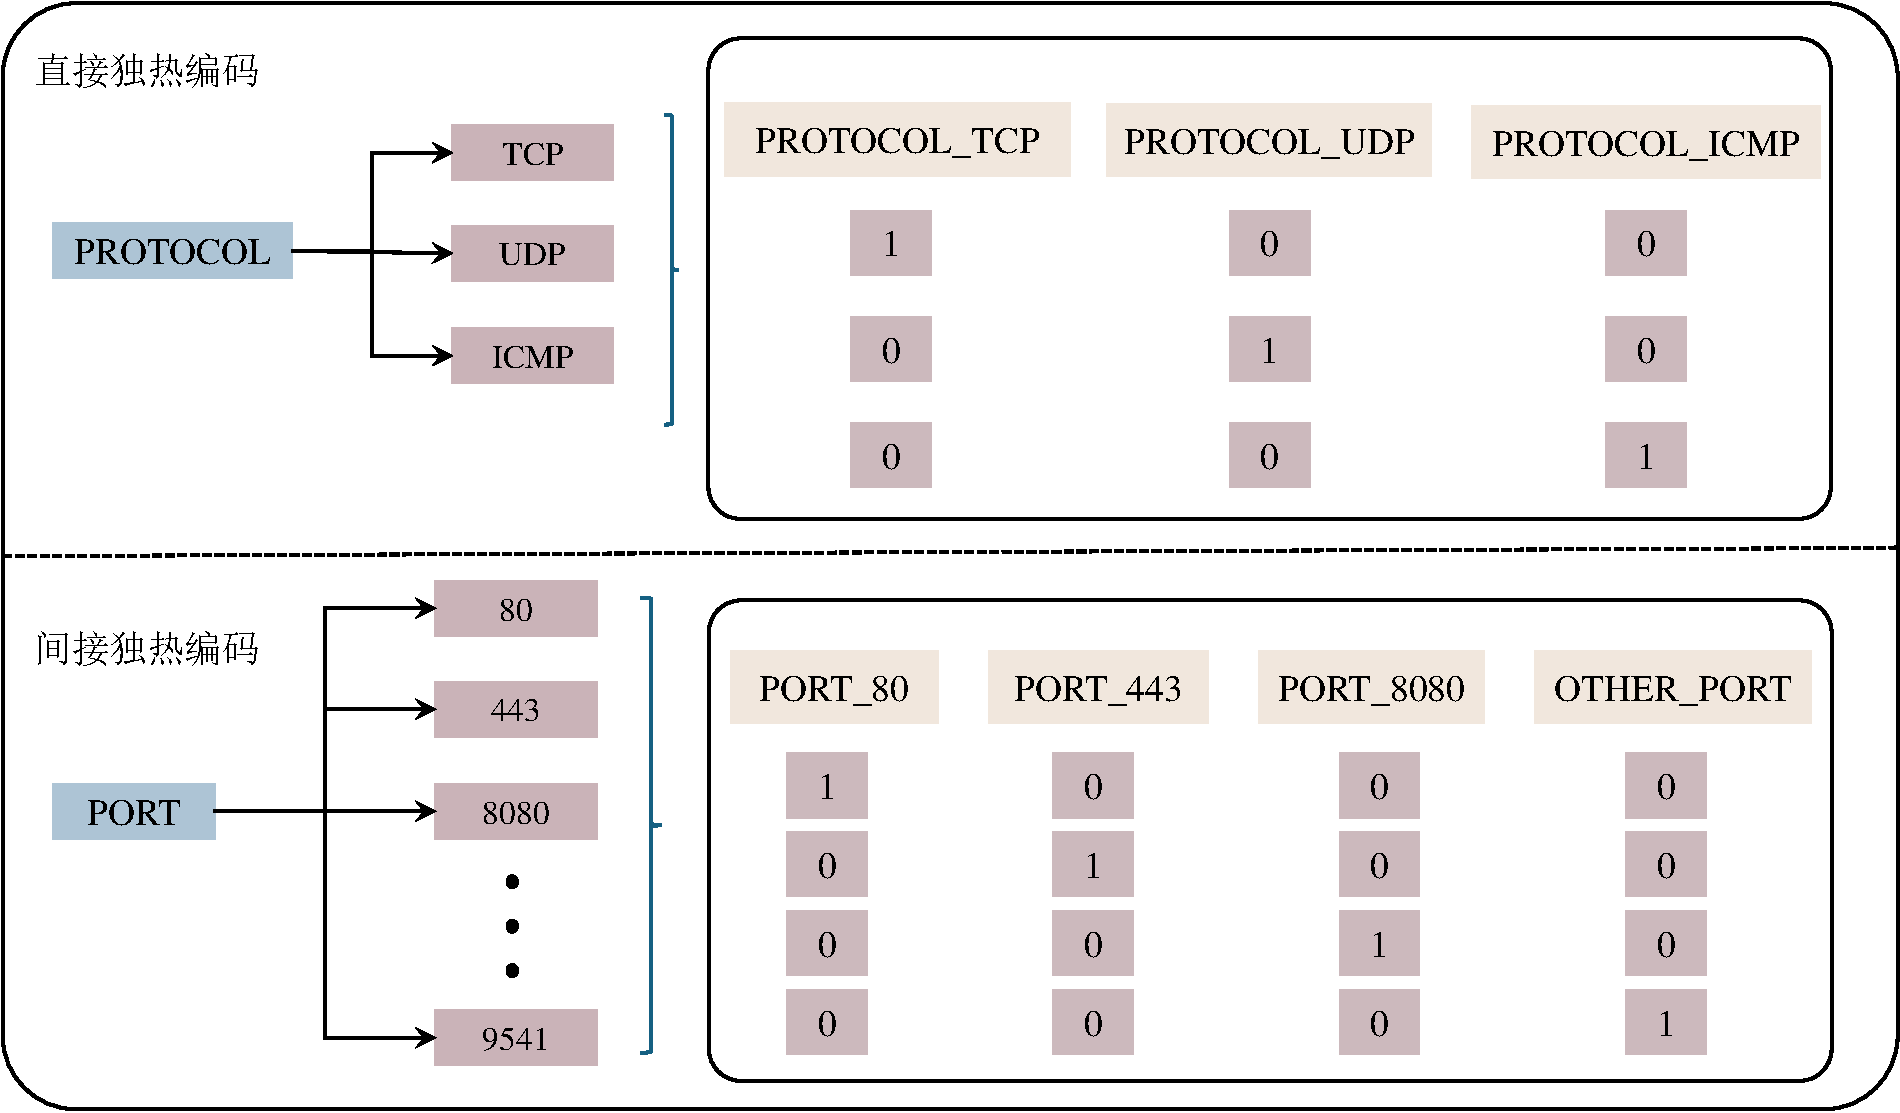
\includegraphics[width=1\linewidth]{./pic/one hot coding(大字版).pdf}
    \caption{两种独热编码方式}
    \label{oneHotCode}
\end{figure}
为了确保编码后的特征能被有效处理,本文采取了两种独热编码方式,如图\ref{oneHotCode}所示。对于类别取值较少且相对固定的特征,如 PROTOCOL、TCP\_FLAGS、DNS\_QUERY\_TYPE 等,直接采用标准的独热编码方法。即,为每个类别的不同取值创建独立的二元特征列,表示该类别是否属于某一特定值。这种方法能够明确表达各类别之间的不同,有助于模型更精确地捕捉流量中的模式。对于一些取值众多且频率不均的特征,如PORT、 L4\_SRC\_PORT、L4\_DST\_PORT、L7\_PROTO、ICMP\_TYPE 等,直接进行独热编码可能会导致特征维度过大,进而增加计算复杂度。因此,采用间接独热编码方法。具体来说,首先统计这些特征中出现频率较高的前 n 个取值,并为这些取值创建新的二元特征列,而将剩余不常见的取值归为一个“Other”类别。这样不仅减少了特征维度,还确保了编码后的特征能够代表大部分常见流量模式,同时避免了高维度带来的计算开销。
最后,为了确保不同特征具有相同的尺度,从而避免某些特征因为数值范围大而在模型训练过程中占据主导地位。例如网络流量数据中,“输入字节数(IN\_BYTES)”可能在几千到几百万之间,而“TTL值(MIN\_TTL)”则在1到255之间。如果不进行归一化处理,数值范围较大的特征可能会对模型的训练产生更大的影响,从而导致模型对某些特征的偏倚。本研究采用QuantileTransformer对连续性特征进行归一化操作,QuantileTransformer的过程可以分为一下几个步骤:排序数据并计算分位数,如公式\ref{p_i}所示;将数据点的分位数映射到目标分布(如均匀分布或正态分布),如公式\ref{x_i}所示;逆变化,将数据恢复到原始分布,如公式\ref{x_ii}所示。
\begin{equation}
p_i = \frac{i}{n}, \quad \text{for} \quad i = 1, 2, \dots, n
\label{p_i}
\end{equation}
\begin{equation}
x_i = F_{\text{normal}}^{-1}(p_i) = \Phi^{-1}(p_i)
\label{x_i}
\end{equation}
\begin{equation}
x_i' = F_{\text{normal}}(x_i) = \Phi(x_i)
\label{x_ii}
\end{equation}
此外,在网络流量分析和恶意流量检测中,标签数据的稀缺性和人工标注成本的高昂,往往限制了传统监督学习方法的应用。为了解决这一问题,半监督学习(Semi-supervised Learning)方法成为了一种有效的解决方案。半监督学习通过同时利用少量的标记数据和大量的未标记数据进行训练,从而能够在标签稀缺的情况下,获得较为准确的分类结果。这种方法特别适用于标签数据不平衡或数据难以标注的场景。具体来说,半监督学习方法在训练过程中,首先利用已标记数据进行监督学习,然后通过推测未标记数据的标签来增强学习过程。通过这种方式,有效地利用了未标记数据中的结构信息,进而提升了模型的分类性能。

在本研究中,将数据集划分为70\%用于训练,30\%用于测试。此划分策略旨在最大化利用标记数据训练模型,同时保持测试集的独立性,确保模型性能评估的准确性。为了实现半监督学习,采用了基于图的半监督学习方法。在这种方法中,将数据表示为图的形式,其中每个节点代表网络中的设备或IP地址,而边则表示设备之间的通信关系。图神经网络通过对图结构的学习,能够对节点之间的复杂关系进行建模,并在传播信息的过程中逐步推断未标记节点的标签。这一过程不仅能够学习到每个节点的特征,还能够通过图中的拓扑结构捕捉到未标记数据的潜在标签信息,从而提高分类性能。

基于图的半监督学习方法相较于传统的机器学习方法具有明显优势,尤其在面对具有复杂关系和时序性的数据时。网络流量数据通常包含了丰富的时序信息和设备间复杂的通信拓扑,传统的机器学习方法往往无法充分利用这些信息。而图神经网络通过传播节点间的信息,能够有效地捕捉到这些复杂的关系。此外,图神经网络还能够处理稀疏数据和不规则结构,这对于网络流量分析尤为重要,因为流量数据中往往存在不完全的标注或异常数据,图神经网络可以利用图的结构关系来补充这些缺失的信息,如图\ref{halfsuppervised}所示。

\begin{figure}[h!]
    \centering
    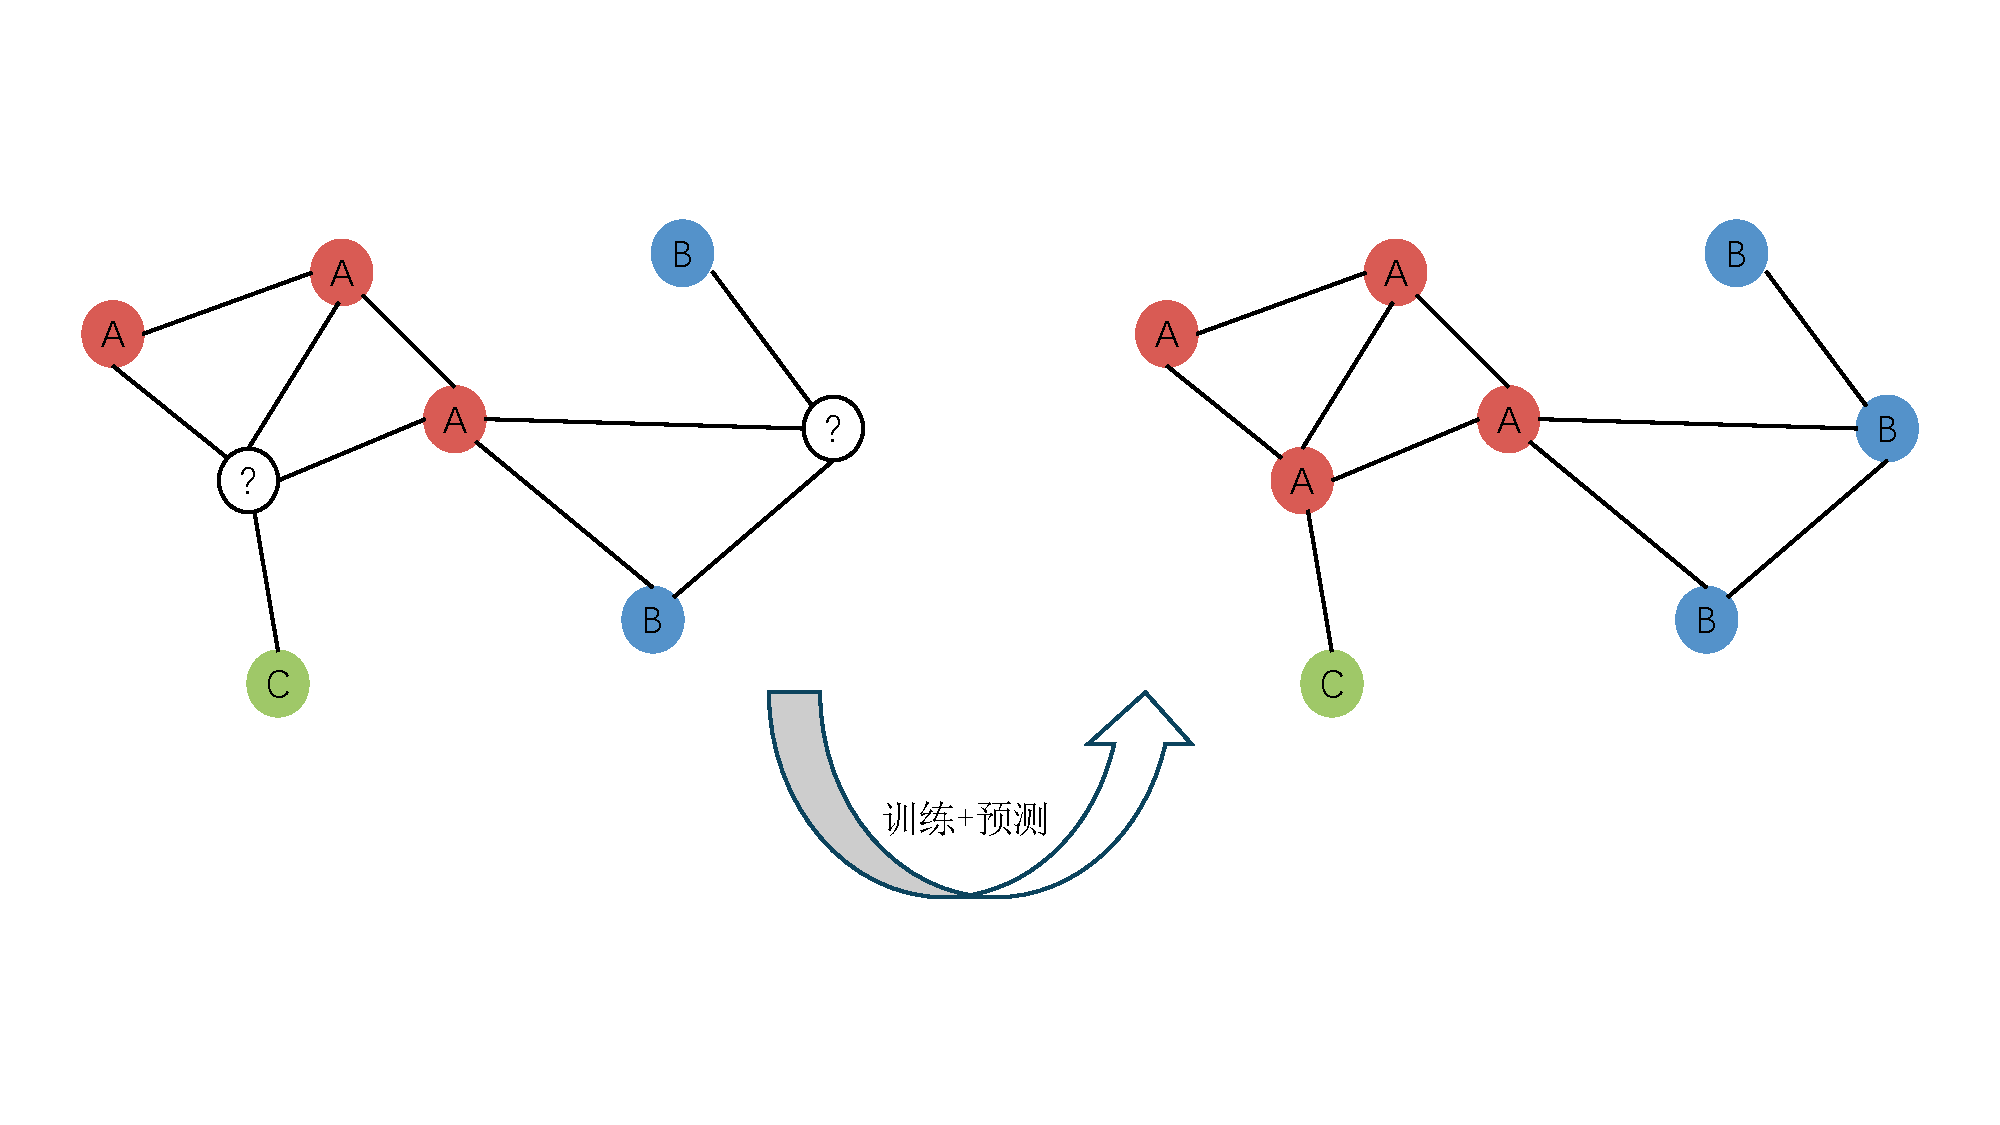
\includegraphics[width=1\linewidth]{./pic/基于图半监督学习方法(大字版).pdf}
    \caption{图半监督学习}
    \label{halfsuppervised}
\end{figure}
此外,半监督学习方法的引入解决了标签数据不足的问题。在传统的监督学习方法中,获取标注数据成本高且耗时,是模型训练的一大挑战。通过半监督学习,模型可以在大量未标记数据的基础上进行训练,从而减少了对标记数据的依赖,并能够提高数据的利用率。基于图的半监督学习方法,不仅提升了流量分类的准确性,还通过信息传播机制,改善了对少量标记数据的依赖,使得模型能够在标签稀缺的情况下有效地训练。


为了应对日益复杂的网络攻击行为,传统的入侵检测方法已无法满足对长期、持续性攻击的有效识别需求。尤其是针对持续时间较长的攻击,如DDoS攻击或暴力破解等,网络流量的特征通常会随时间发生动态变化,因此,需要一种能够捕捉到这些时间演化特征的检测方法。本文采用时序图的构建与分析方法,旨在通过时序图捕捉网络流量的演化过程,进而实现对潜在攻击行为的精准检测。
\subsection{时序图构建}
\begin{figure}[h!]
    \centering
    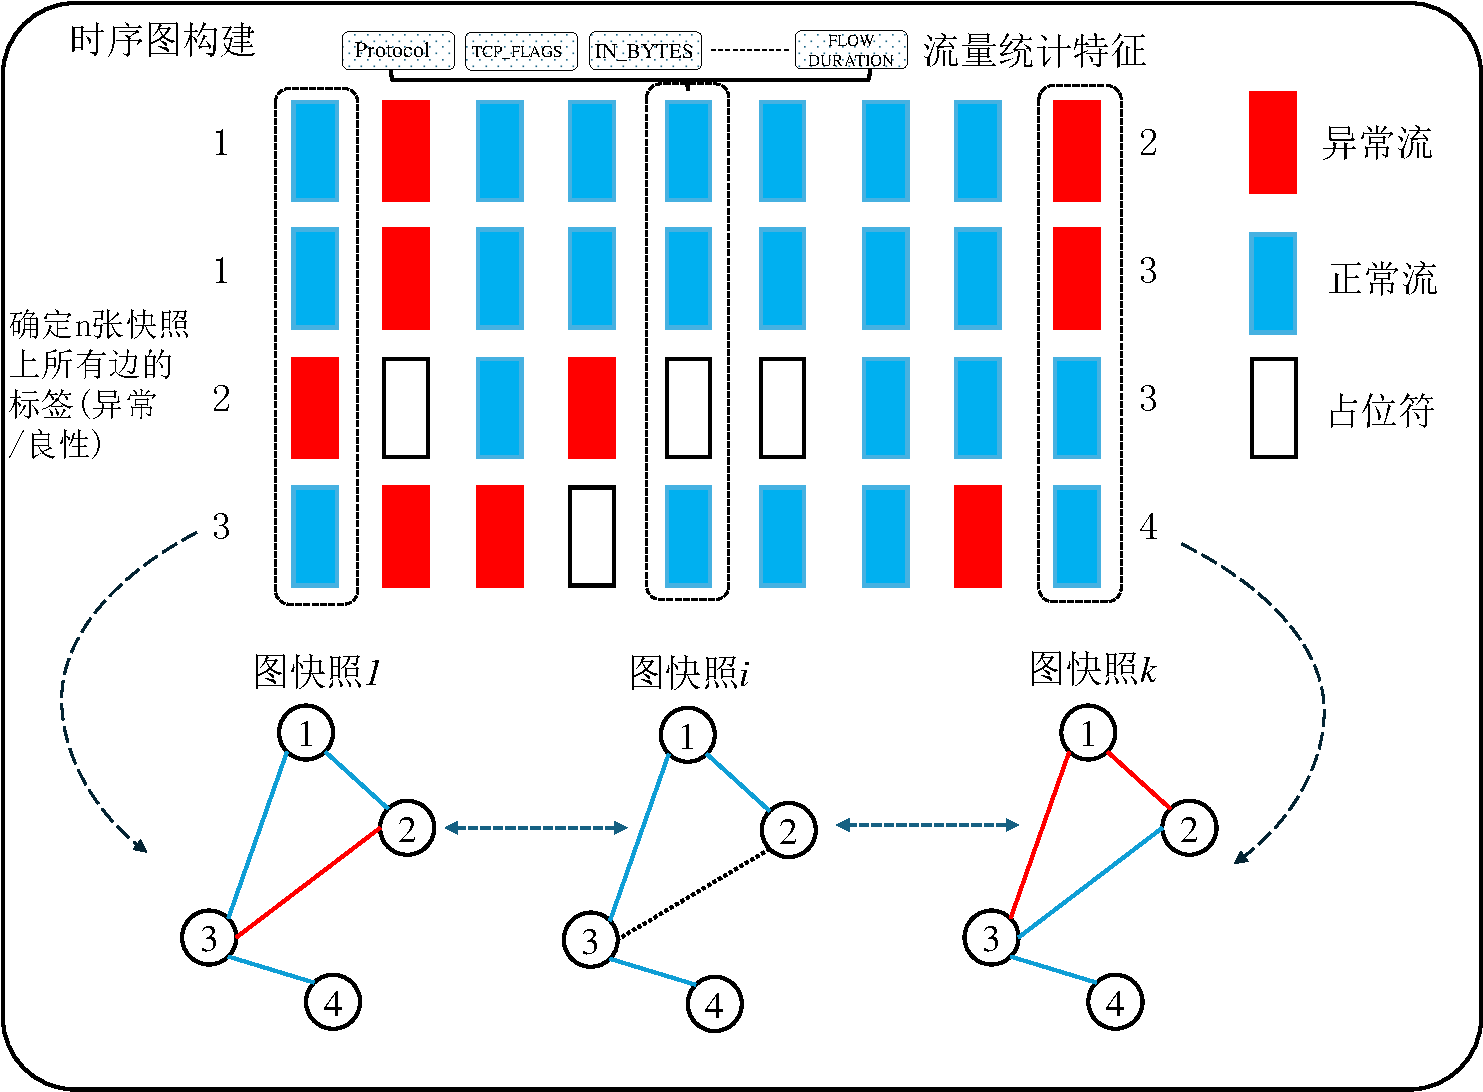
\includegraphics[width=1\linewidth]{./pic/SpatiotemporalGraph(大字版).pdf}
    \caption{时序图构建}
    \label{SpationtemporalGraph}
\end{figure}

每个图快照由节点集合 \( V_f \) 和边集合 \( E_f \) 组成。节点集合 \( V_f \) 代表在该时刻参与通信的所有IP地址,而边集合 \( E_f \) 则表示在该时刻存在流量的IP地址对之间的连接,每条边的特征包括流量的协议类型、持续时间、入站流量字节数、每包字节数、TCP标志位等。这些特征不仅描述了网络流量的属性,而且可以用来识别流量的正常性与异常性。例如,Zhang 等人\citing{zhang2022realtime}提出了一种基于图模型的入侵检测方法,强调了流量特征在攻击检测中的重要性。
\begin{equation}
A_{ij}^f = \begin{cases} 
1 & \text{如果 } (v_i^f, v_j^f) \in E_f \\
0 & \text{否则}
\label{a_ij}
\end{cases}
\end{equation}

时序图的构建首先依赖于网络流量数据的转换,如图\ref{SpationtemporalGraph}所示。具体来说,网络流量是由成对的IP地址之间的通信构成的双向流量,而每一对IP地址之间的通信可以视为图中的一条边,IP地址则对应图中的节点。在此框架下,将网络流量数据按照时间戳切割成多个图快照,构成时序图序列。每一个图快照代表某一时刻的网络拓扑结构,通过时间顺序连接这些图快照,可以表达网络流量的动态变化。类似的图结构在网络分析中已经得到了广泛应用。


为了便于后续的图分析和模型训练,图的拓扑结构通过邻接矩阵表示。对于第 \( f \) 个快照 \( G_f = (V_f , E_f) \),其邻接矩阵 \( A_f \) 是一个 \( N \times N \) 的矩阵,其中 \( N \) 是网络中IP地址的数量。如公式\ref{a_ij}所示,其中 \(A_{ij}^f = 1\) 表示节点 \(v_i^f\) 与节点 \(v_j^f\) 之间存在边,反之 \(A_{ij}^f = 0\) 表示无边。如果在第 \( f \) 个图快照中,这两个节点之间有通信流量,则 \( A_{ij}^f = 1 \),否则为0。这种邻接矩阵的表示方式简洁而有效,能够直接反映网络中各个IP地址之间的连接关系,并为图分析模型提供输入。

时序图的核心优势在于能够反映网络流量随时间的演化。现实中,DDoS攻击等攻击行为往往是一个持续的过程,攻击流量会随着时间的推移逐渐增加,这导致网络拓扑和流量特征发生变化。通过将每个时刻的网络状态表示为一个静态图,并将这些静态图按时间顺序连接成时序图,能够有效追踪网络流量的动态变化。具体来说,假设有 \( K \) 个图快照 \( G_1, G_2, \dots, G_K \),这些快照反映了从 \( t_1 \) 到 \( t_K \) 时刻的网络状态。通过分析这些图快照的演化过程,可以揭示网络流量中的长期依赖关系,进而更好地捕捉到潜在的攻击行为。类似的研究已经表明,时序图能够有效建模流量的演变过程,进而实现对网络攻击的更精确检测。
在恶意流量检测任务中,流量特征随着时间的推移会发生变化,特别是在攻击期间。为了捕捉这些时序依赖关系,图中的边特征会随时间演化,如公式\ref{e_ij}所示。假设第 \(f\) 到第 \(f+t\) 个图快照中的边特征分别为 \(\{ e_{ij}^f, e_{ij}^{f+1}, \dots, e_{ij}^{f+t} \}\),则流量的变化可以表示为这些边特征的演变。图神经网络能够通过学习这些时序依赖关系,进一步提升流量检测的精度。
\begin{equation}
e_{ij}^{f+t} = f(e_{ij}^f, \dots, e_{ij}^{f+t})
\label{e_ij}
\end{equation}

其中,\(f\) 表示流量特征随时间变化的函数。通过图的演化,时序图能够捕捉到攻击的长期演变特征,帮助识别持续性攻击。

时序图还能够处理网络流量中的稀疏性问题。在实际网络环境中,流量往往不是均匀分布的,设备可能会因故障或其他原因暂时断开连接,或是某些时间段内没有数据传输。为了应对这种稀疏性,通常会在缺失的图快照中插入占位符。占位符的作用是填补网络流量的空白时刻,以确保图的时序性和完整性。具体而言,将占位符边的特征设置为0,并通过特殊标签标记这些边。通过这种方式,可以保持图的结构不受缺失数据的影响,从而保证时序图的完整性。

此外,时序图还能够有效捕捉到网络攻击的演化特征。网络攻击通常不是突然发生的,而是一个逐步演变的过程。
例如,在DDoS攻击期间,攻击流量通常从低谷逐渐上升,直到达到峰值。这种攻击模式在时序图中表现为边特征的逐步变化,
时序图能够准确捕捉到这种演化过程。通过分析图的演化,能够有效区分正常流量与攻击流量,识别出攻击的发生及其持续时间。
已有研究表明,时序图能够显著提高对这种持续性攻击的检测能力。
时序图还为半监督学习提供了有效的支持。在实际应用中,由于标签数据的匮乏,半监督学习方法能够在少量标记数据的基础上进行训练,并在未标记数据上进行验证。在时序图的训练过程中,通过标记少量的边,可以对整个时序图中的所有边进行检测,识别出潜在的异常行为。由于时序图能够捕捉到网络流量的长期依赖性和时序演化,半监督学习方法能够利用这些信息有效提高检测的准确性,特别是在面对持续性攻击时,时序图提供了比传统方法更为精细的分析能力。

时序图通过其时间维度上的演化特点,能够精准地捕捉到攻击行为的变化过程,尤其在面对DDoS攻击、暴力破解等持续性攻击时表现出色。通过构建时序图并结合半监督学习模型,可以有效地识别出攻击行为,提升入侵检测系统的性能和准确性。为了成功构建出时序图,本文采用了算法\ref{createTimeGraph}生成时序图集,首先,算法接受多个图快照 $G_1, G_2, \dots, G_K$,每个图快照由节点集合 $V_f$ 和边集合 $E_f$ 组成,表示在不同时间点上网络的拓扑结构和流量信息。其次,对于每一对 IP 地址 $(v_i, v_j)$,算法计算它们之间的双向流量特征,例如协议类型、流量持续时间、字节数等。若该对 IP 地址之间存在流量连接,则在相应的图快照中创建边,并记录相关的流量特征。然后,算法为每个图快照构建邻接矩阵 $A_f$,该矩阵表示图中各个节点(IP 地址)之间的连接关系。如果两个节点之间存在流量连接,则矩阵中对应元素设为 1,否则设为 0。最后,由于实际网络中流量分布存在不均匀性,某些时刻可能缺失图快照。为了处理这种稀疏性,算法在缺失位置插入占位符边,并将这些边的特征设为 0,从而保持时序图的完整性。
\begin{algorithm}[h!]
\caption{时序图构建算法}
\label{createTimeGraph}
\KwIn{$K$ 个图快照 $G_1, G_2, \dots, G_K$,每个图快照包含节点集合 $V_f$ 和边集合 $E_f$}
\KwOut{时序图 $T = \{G_1, G_2, \dots, G_K\}$}
\For{$f = 1$ \textbf{to} $K$}{
    \ForEach{每对 IP 地址 $(v_i, v_j)$}{
        计算该对 IP 地址之间的双向流量特征\;
        记录流量的协议类型、持续时间、字节数、TCP 标志等特征\;
        \eIf{存在流量连接}{
            在图快照 $G_f$ 中创建边 $(v_i, v_j)$ 并记录其流量特征\;
        }{
            跳过此对 IP 地址\;
        }
    }
    \ForEach{每个图快照 $G_f$}{
        构建邻接矩阵 $A_f$,其中 $A_{ij}^f$ 表示节点 $v_i$ 和节点 $v_j$ 是否连接\;
        \eIf{流量连接存在}{
            设置 $A_{ij}^f = 1$\;
        }{
            设置 $A_{ij}^f = 0$\;
        }
    }
}
\For{$f = 1$ \textbf{to} $K$}{
    \ForEach{图快照中的空缺位置}{
        插入占位符边,所有特征值设为 0\;
        使用特殊标签标记该边为占位符\;
    }
}
\end{algorithm}

\subsubsection{时序粒度适应与滑动窗口机制}

在实际网络环境中,时序粒度的选择对攻击检测性能具有重要影响。时序粒度过粗会导致无法捕捉到攻击行为的短时突发特征,
而粒度过细又可能导致数据稀疏、图连通性差、噪声增加,从而影响模型的稳定性与准确性。
为了在不同时间尺度下更好地构建时序图,本文引入了滑动窗口机制和重叠率控制策略,以自适应地优化时序粒度。

具体地,采用固定长度的滑动窗口对连续网络流量数据进行分段构建图快照,通过调整窗口重叠率,
来控制相邻图快照之间的数据重叠程度。较高的重叠率可以在保持时序连续性的同时,增加训练样本量,
缓解数据稀疏问题,提升图连通性和特征平滑性。同时,滑动窗口机制能够在不同尺度上观察网络状态演化,
有效捕捉到攻击流量的局部变化与异常行为。

该设计不仅增强了时序图的表达能力,也提升了模型在长时间序列中的鲁棒性与检测准确率。后续将在第四章实验部分通过不同窗口大小与重叠率的对比实验,进一步验证该机制的有效性。



\subsection{基于LDNFDDPM恶意流量生成}
旨在生成高度逼真的恶意攻击数据,以接近实际场景,时序图的构建不仅需要关注图的拓扑结构和时序关系,还需要特别关注流量数据的特征选择。根据恶意攻击流量的特点,特征选择过程细化为保留功能性特征(\( x_f \))并生成非功能性特征(\( x_{nf} \)),最后再增加低度IP的权重,如图\ref{LDNFDDPM}所示。这种方法能够确保生成的数据在保留关键特征的基础上,增加数据多样性,提升模型对真实世界的适应力和预测精度。
功能性特征是指那些对恶意攻击流量分类有显著影响的特征,这些特征通常能够反映攻击流量的核心特征和模式。例如,源IP(Src IP)、目标IP(Dst IP)、协议类型(Protocol)、目标端口(Dst Port)等都被认为是功能性特征。这些特征在流量分析中具有明确的指示作用,通过它们可以快速区分不同类型的攻击和正常流量。因此,在数据增强过程中,这些特征通常被保留下来,确保生成的流量样本能够尽可能地模拟真实的攻击模式。

另一方面,非功能性特征是指那些对攻击类型的分类影响较小,或者可以通过生成模型推测的特征。
例如,流量的字节数、数据包数量、流的持续时间等。
虽然这些特征对流量的细节描述很重要,
但它们更多地与网络状态和时序行为相关,不一定直接影响攻击的识别。
因此,非功能性特征通常会通过生成模型来生成,以增加数据的多样性,尤其是在数据稀缺和标签不平衡的情况下。
\begin{figure}[h!]
    \centering
    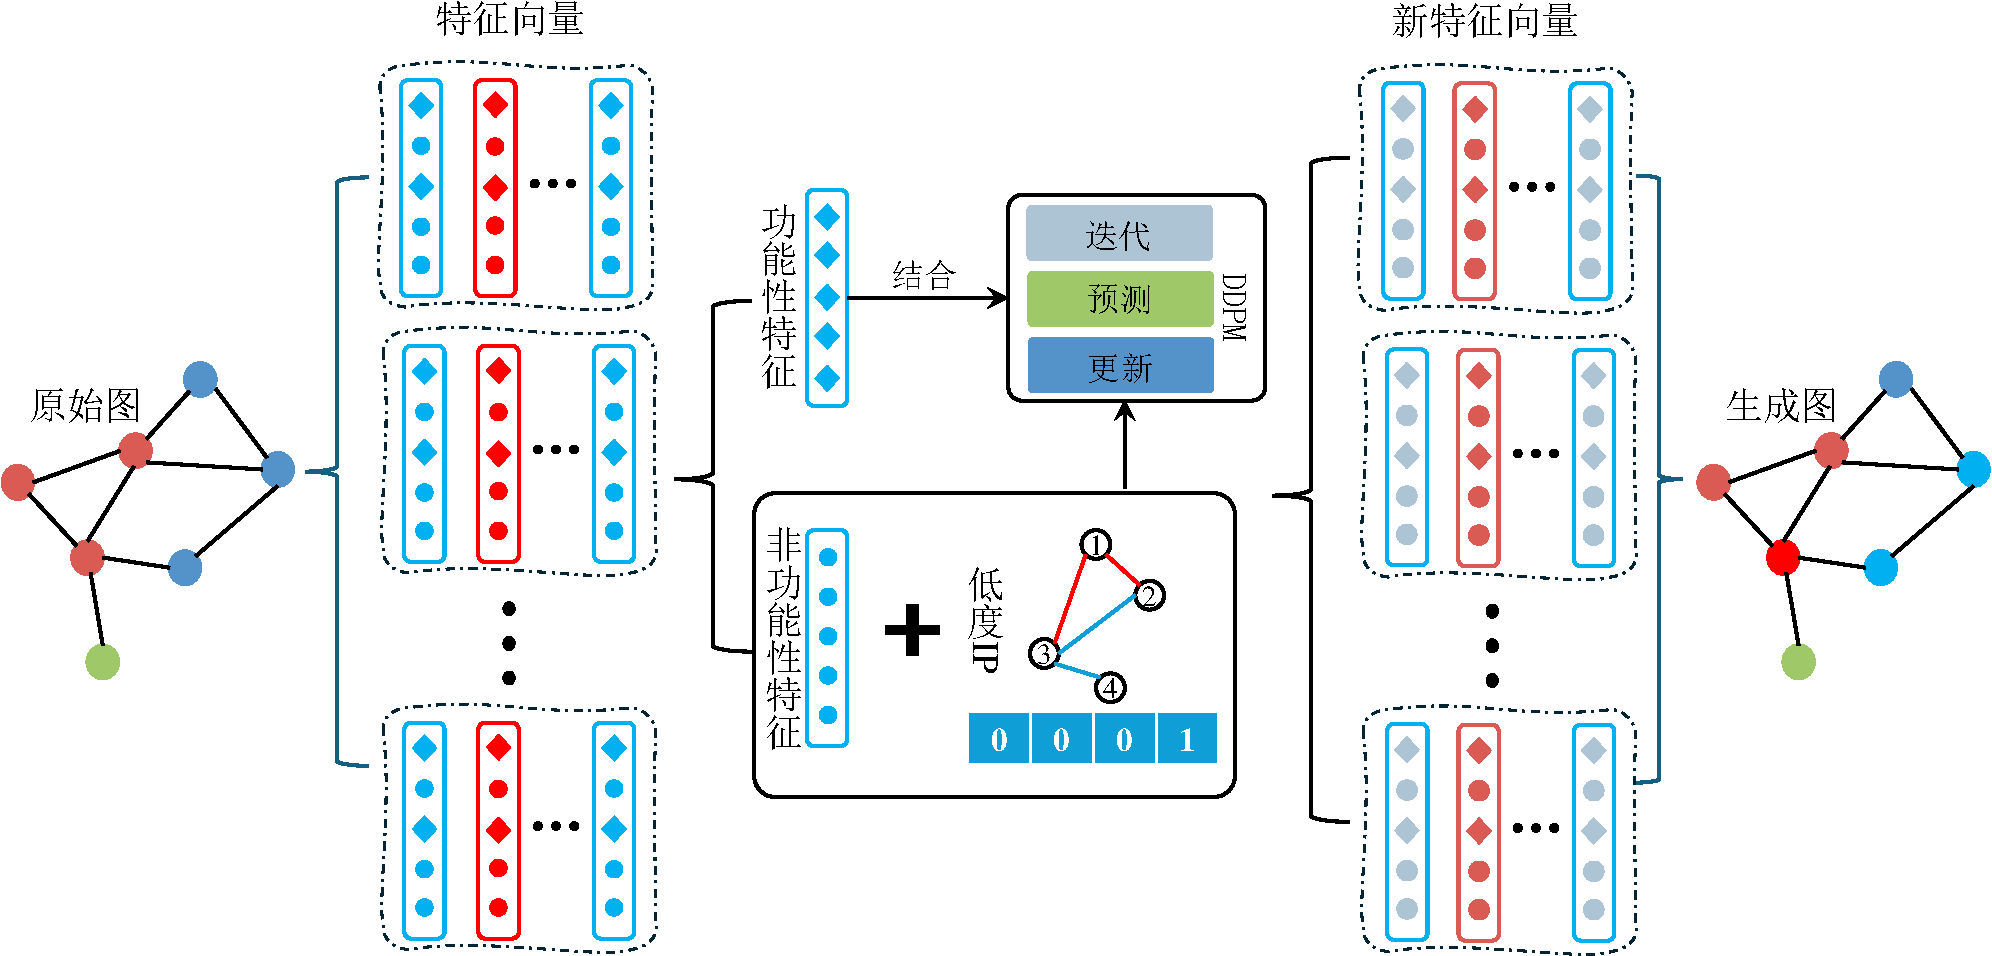
\includegraphics[width=1\linewidth]{./pic/LDNFDDPM(大字版).pdf}
    \caption{LDNFDDPM}
    \label{LDNFDDPM}
\end{figure}

为了确保生成的攻击流量数据逼近真实数据,首先需要从实际攻击流量数据中选择出那些最具代表性的功能性特征。
为了量化每个特征的贡献,可以采用随机森林算法计算每个特征的重要性。随机森林通过训练多个决策树并综合各个树的输出,能够有效评估每个特征对攻击类型分类的贡献度。随机森林的训练过程可以表示为:
\begin{equation}
\hat{y} = \frac{1}{N} \sum_{n=1}^{N} h_n(x)
\end{equation}

其中,\( \hat{y} \) 是预测值,\( N \) 是决策树的数量,\( h_n(x) \) 是第 \(n\) 棵树的预测函数。通过计算每棵树中各特征的贡献度,可以确定每个特征的重要性。

通过这种方式,随机森林能够自动识别出在不同攻击类型下最有助于分类的特征。例如,在DDoS攻击中,源IP和目标IP可能具有较高的重要性,而在网络嗅探攻击(如Reconnaissance)中,协议类型和目标端口可能会更加重要。因此,在特征选择过程中,随机森林算法能够帮助选择出最重要的功能性特征,确保生成的流量数据更具代表性和准确性。

对于非功能性特征,由于其在流量分类中的作用较小,可以通过DDPM等生成模型进行数据增强。DDPM通过在多个步骤中逐渐去噪,能够生成与原数据相似的样本,特别是在数据稀缺和标签不平衡的情况下,DDPM能够有效扩展训练数据集。具体而言,DDPM模型在每个时间步骤 \(t\) 上加入噪声,并学习如何从噪声中恢复原始数据:
\begin{equation}
x_t = \sqrt{\bar{\alpha_t}} x_0 + \sqrt{1 - \bar{\alpha_t}} \epsilon
\end{equation}

其中,\(x_0\) 是原始数据,\(x_t\) 是加噪后的数据,\(\epsilon\) 是从标准正态分布中采样的噪声,\(\bar{\alpha_t}\) 是与噪声扩散相关的预定义时间表。

在训练过程中,DDPM通过优化以下目标函数来学习去噪过程:
\begin{equation}
\mathcal{L}(\theta) = \mathbb{E}_{x_0, t} \left[ \left\| \epsilon_\theta(x_t, t) - \epsilon \right\|^2 \right]
\end{equation}

其中,\(\epsilon_\theta(x_t, t)\) 是去噪网络的输出,\(\epsilon\) 是真实的噪声。通过这种方式,DDPM能够生成逼近真实攻击流量的非功能性特征,并扩充数据集。

在生成过程中,功能性和非功能性特征需要分别进行处理。对于功能性特征,保留原始的数值,
而对于非功能性特征,利用DDPM进行生成。具体来说,每个攻击类型会对应一组特征,其中将功能性特征保留下来,非功能性特征则通过DDPM生成并填补。

为了确保生成的非功能性特征既符合实际流量模式,又能扩展数据集的多样性,我们采用了以下约束策略:

(1)基于历史流量模式的统计约束:在生成非功能性特征时,首先对正常流量和攻击流量的字节数、数据包数量等统计特征进行分析,得出其概率分布。
生成模型将在这些统计约束的指导下生成符合实际流量特点的特征。

(2)条件生成:针对不同类型的攻击,使用条件生成模型(如条件DDPM)生成符合攻击类型特点的非功能性特征。
例如,DDoS攻击通常涉及大量的流量,而Reconnaissance攻击则相对较少。因此,生成时考虑攻击类型的上下文信息,以确保生成的数据符合攻击的特性。

(3)正则化约束:通过引入KL散度等正则化方法,在训练过程中对生成的特征进行约束,避免生成无意义或不符合实际规律的特征。
这样可以保证生成的流量数据既具备多样性,又符合现实情况。

每个流量特征视为随机变量来考虑,且每个特征服从某种未知的联合分布。每条流量数据的特征向量可以表示为:
\begin{equation}
x_i = \{ q_{i,1}, q_{i,2}, \dots, q_{i,m} \}, \quad i \in \{1, 2, \dots, n\}
\end{equation}
其中,\(x_i\) 是第 \(i\) 条流量数据的特征向量,包含 \(m\) 个特征。原始的流量数据集 \(S\) 可以定义为:
\begin{equation}
S = (x, y)
\end{equation}
其中,\(x\) 代表样本的特征向量,\(y\) 是样本的标签,取值范围为 \(\{0, 1, \dots, k\}\),其中 \(y = 0\) 表示良性数据,\(y = 1\) 到 \(y = k\) 表示恶意攻击数据,\(k\) 的取值由恶意攻击的种类决定。

进一步地,可以将每个特征向量划分为功能性特征 \(x_i^f\) 和非功能性特征 \(x_i^{nf}\),如下所示:
\begin{equation}
x_i = \underbrace{\{ q_{i,1}, q_{i,2}, \dots, q_{i,u} \}}_{x_i^f} \cup \underbrace{\{ q_{i,u+1}, \dots, q_{i,m} \}}_{x_i^{nf}}, \quad i \in \{1, 2, \dots, n\}
\end{equation}
其中,\(u\) 表示所选取的功能性特征的个数。划分后的数据集 \(S_{nf}\) 定义为:
\begin{equation}
S_{nf} = (x_{nf}, y)
\end{equation}
其中,\(x_{nf}\) 是去掉功能性特征后的非功能性特征部分,\(y\) 是标签。

DDPM模型通过采样得到的非功能性特征将与保留下来的功能性特征结合,形成最终的流量特征向量。这样,生成的恶意流量不仅具备攻击流量的核心特征,还在非功能性特征上具有多样性,从而增强了生成数据的真实感和多样性。

在流量图中,低度IP通常表示与其他IP的通信较少,可能代表某些异常或攻击行为。为了更好地处理这部分流量数据,可以根据IP的度数(连接数)来识别低度IP。具体而言,对于某一IP \(i\),其度数 \(d_i\) 可以通过以下公式计算:
\begin{equation}
d_i = \sum_{j} \mathbb{I}(e_{ij}^f)
\end{equation}

其中,\(\mathbb{I}(e_{ij}^f)\) 为指示函数,表示在图快照 \(f\) 中,节点 \(i\) 和节点 \(j\) 是否有边相连。当 \(d_i\) 小于某个阈值 \(T\) 时,该IP视为低度IP。

\begin{algorithm}[h!]
\caption{低度IP处理算法}
\label{LowDegreeIP}
\KwIn{图数据集 graph}
\KwOut{处理后的图数据集 data}
\BlankLine
读取预处理的数据,构建图结构\;
\For{每个节点 $i$}{
    计算节点 $i$ 的度数\;
    \If{度数小于阈值 $T$}{
        标记节点 $i$ 为低度IP\;
    }
}
生成低度IP掩码\;
\For{每个低度IP}{
    进行特征生成和加权平均\;
}
更新图数据集\;
\Return 处理后的图数据集 data\;
\end{algorithm}
生成过程中,针对低度IP的流量,特别加以关注。通过构建低度IP的掩码,并在生成过程中对这些掩码位置进行特征生成,能够增加模型对低度IP流量的敏感性,进一步增强数据的真实性。具体过程如算法\ref{LowDegreeIP}所示。

通过特征的功能性与非功能性划分,结合DDPM生成非功能性特征,可以有效扩充恶意攻击流量的数据集,尤其是在面对数据不平衡和标签稀缺的情况下,数据增强方法能够显著提高模型的性能。功能性特征的保留确保了生成的数据具有代表性,而非功能性特征的生成则增加了数据的多样性,为恶意流量检测提供了更多的信息和支持。

\section{实验分析}
本章在三个流行的网络流量数据集上来验证提出的方法在数据增强上的效果。
\subsection{实验设置}

本文所提的LDNFDDPM和LG-MTD方法在配备3.50GHz的12核Intel(R)\\Core(TM)i9-10920X
 CPU、256 GB 内存和Linux 内核v.5.11.0 的 Ubuntu 20.04 LTS 操作系统上进行评
估。选用PyTorchv1.7.0 与 Jupyter notebook 一起实现相关实验,具体实验设置如
表\ref{tbl:hardware_config}所示。
\begin{table}[h!]
    \centering
    \caption{硬件配置}
    % \resizebox{\textwidth}{!}{
    \begin{tabular}{c||c} \hline\hline
        \textbf{名称} & \textbf{配置} \\ \hline
        CPU & i9-10920X \\ \hline
        GPU & 技嘉RTX3080 \\ \hline
        内存 & 镁光256GB 3200HZ 8 \\ \hline
        硬盘 & 三星2TB 2 \\ \hline\hline
    \end{tabular}
    \label{tbl:hardware_config}
    % }
\end{table}

\subsection{实验数据}

\begin{table}[h!]
    \centering
    \caption{NF-BoT-IoT-V2 数据集主要属性}
    \begin{tabular}{c||c} \hline\hline
        \textbf{属性} & \textbf{描述} \\ \hline
        流量总数 & 37,763,497 \\ \hline
        良性流量比例 & 0.36\% \\ \hline
        IP 地址数 & 293 \\ \hline
        端口数量 & 65,536 \\ \hline
        平均流持续时间 & $3.999 \times 10^6$ 毫秒 \\ \hline
        平均输入字节数 & 546 \\ \hline
        平均输出字节数 & 204 \\ \hline
        TCP 标志数量 & 25 \\ \hline
        支持协议类型 & ICMP、TCP、UDP \\ \hline
        攻击类别 & Reconnaissance, DDoS, DoS, Theft  \\ \hline\hline
    \end{tabular}
    \label{tbl:nf_bot_iot_v2}
\end{table}
本文采用NF-BoT-IoT-V2、NF-ToN-IoT-V2、NF-CSE-CIC-IDS2018-V2三个数据集\citing{sarhan2022towards},详细介绍如下:

NF-BoT-IoT-V2 数据集是基于原始 BoT-IoT 数据集生成的,如表\ref{tbl:nf_bot_iot_v2}所示。BoT-IoT 数据集最初由澳大利亚国立计算机安全中心(ACCS)实验室创建。通过使用 nProbe 提取原始 PCAP 数据中的 43 个 NetFlow 特征,生成了该数据集。NF-BoT-IoT-V2 包含 37,763,497 条流量数据,其中良性流量比例仅为 0.36\%,其余均为攻击流量。该数据集覆盖了 293 个 IP 地址和 65,536 个端口,平均流持续时间为 $3.999 \times 10^6$ 毫秒。它的入站和出站流量字节数较低,分别为 546 和 204。其主要支持的协议类型包括 ICMP、TCP 和 UDP。NF-BoT-IoT-V2 的攻击类型涵盖了探测攻击、DDoS 攻击、DoS 攻击以及数据盗窃。作为物联网流量分析的一个重要数据集,NF-BoT-IoT-V2 在攻击类型和规模上具有显著的失衡性,适合用于异常检测和攻击分类的研究。

\begin{table}[h!]
    \centering
    \caption{NF-ToN-IoT-V2 数据集主要属性}
    \begin{tabular}{c||c} \hline\hline
        \textbf{属性} & \textbf{描述} \\ \hline
        流量总数 & 16,940,495 \\ \hline
        良性流量比例 & 36.01\% \\ \hline
        IP 地址数 & 29,245 \\ \hline
        端口数量 & 65,536 \\ \hline
        平均流持续时间 & $7.929 \times 10^5$ 毫秒 \\ \hline
        平均输入字节数 & 726 \\ \hline
        平均输出字节数 & 837 \\ \hline
        TCP 标志数量 & 34 \\ \hline
        支持协议类型 & ICMP、TCP、UDP、IPv6-ICMP \\ \hline
        攻击类别 &  DDoS, DoS, Backdoor,Injection,Password,Scanning,XSS \\ \hline\hline
    \end{tabular}
    \label{tbl:nf_ton_iot_v2}
\end{table}
NF-ToN-IoT-V2 数据集是 ToN-IoT 数据集的扩展版本,如表\ref{tbl:nf_ton_iot_v2}所示。NF-ToN-IoT-V2 数据集最初由澳大利亚国防部数据61实验室开发,旨在模拟真实物联网环境中的网络流量。该数据集包含 16,940,495 条网络流量,其中良性流量占 36.01\%。与其他物联网数据集相比,NF-ToN-IoT-V2 的流量数据覆盖范围较广,包括 29,245 个 IP 地址和 65,536 个端口,支持的协议类型包括 ICMP、TCP、UDP 和 IPv6-ICMP。平均流持续时间为 $7.929 \times 10^5$ 毫秒,入站和出站流量字节数分别为 726 和 837。NF-ToN-IoT-V2 中的攻击类型与 NF-BoT-IoT-V2 类似,主要包括探测攻击、DDoS 攻击、DoS 攻击和数据盗窃。该数据集具有更高的良性流量比例和丰富的流量特征,适合于物联网环境下的多协议分析和跨网络的异常检测研究。

NF-CSE-CIC-IDS2018-V2 数据集基于原始 CICIDS2018 数据集生成,如表\ref{tbl:nf_cse_cic_ids2018_v2}所示。原始数据集由加拿大网络安全实验室(CIC)和通信安全研究中心(CSE)联合创建,旨在模拟现代企业网络中的攻击行为。该数据集包含 18,893,708 条网络流量,其中良性流量比例为 11.95\%。NF-CSE-CIC-IDS2018-V2 拥有 255,042 个独立 IP 地址和 65,492 个端口,协议类型覆盖范围广,包括 ICMP、TCP、UDP、IPv6-ICMP 和 GRE。平均流持续时间为 $5.746 \times 10^5$ 毫秒,入站和出站字节数分别为 1,812 和 6,913。该数据集的攻击类别多样化,包括暴力破解、僵尸网络、DoS 攻击、DDoS 攻击和渗透攻击等。NF-CSE-CIC-IDS2018-V2 数据集的特点在于其流量特征的多样性和复杂性,是研究企业网络安全威胁检测的重要资源,尤其适用于多种攻击类型的分类和流量分析任务。


\begin{table}[h!]
    \centering
    \caption{NF-CSE-CIC-IDS2018-V2 数据集主要属性}
    \begin{tabular}{c||c} \hline\hline
        \textbf{属性} & \textbf{描述} \\ \hline
        流量总数 & 18,893,708 \\ \hline
        良性流量比例 & 11.95\% \\ \hline
        IP 地址数 & 255,042 \\ \hline
        端口数量 & 65,492 \\ \hline
        平均流持续时间 & $5.746 \times 10^5$ 毫秒 \\ \hline
        平均输入字节数 & 1,812 \\ \hline
        平均输出字节数 & 6,913 \\ \hline
        TCP 标志数量 & 50 \\ \hline\hline
        支持协议类型 & ICMP、TCP、UDP、IPv6-ICMP、GRE \\ \hline
        攻击类别 & BruteForce, Bot, DoS, DDoS, Infiltration \\ \hline\hline
    \end{tabular}
    \label{tbl:nf_cse_cic_ids2018_v2}
\end{table}

针对本章所提方法,采用FID(Frechet Inception Distance)指标来评估数据增强效果。

FID是评估生成模型(如生成对抗网络的生成样本与真实样本之间的相似度)的指标。FID的原理是通过比较两个分布(真实数据和生成数据)在某一预训练网络(如Inception v3)上的特征表示来衡量它们之间的差距。

\subsection{相关对比方法}
根据本文的研究方法和实验数据,选择了近年来的优秀工作进行对比。为了评估 LDNFDDPM 在数据增强方面的效果,将其与其他现有数据增强方法进行了对比,如表\ref{dataAppend}所示:




G-IDS\citing{shahriar2020g}:G-IDS是一种基于GAN生成网络流量数据的技术,专门针对网络物理系统的数据不平衡问题。通过生成合成流量数据,G-IDS 可以增加少数类(如攻击流量)的样本量,从而提高入侵检测系统(IDS)的检测性能。虽然其生成的数据能够缓解数据不平衡的问题,但由于使用的是基本的 GAN,生成的数据可能存在一定的偏差和不足。
\begin{table}[h!]
\centering
\caption{数据增强方法对比}
\resizebox{\textwidth}{!}{
\begin{tabular}{>{\centering\arraybackslash}p{0.33\linewidth}||>{\centering\arraybackslash}p{0.33\linewidth}>{\centering\arraybackslash}p{0.34\linewidth}}  % 设置列宽
\hline\hline
\textbf{方法} & \textbf{描述} & \textbf{优缺点} \\
\hline
G-IDS \citing{shahriar2020g} & 利用基本的 GAN 生成流量数据,缓解数据不平衡问题。 & 生成的数据可能存在一定的偏差,训练效果有限。 \\
\hline
SIGMA \citing{msika2019sigma} & 使用随机森林对特征进行分割并使用 GAN 生成对抗样本。 & 生成的数据可能不能完全捕捉所有攻击流量特征。 \\
\hline
CWGAN-GP \citing{kang2022cwgan} & 基于 Wasserstein 距离的生成对抗网络,加入条件信息来改进数据生成。 & 生成的样本质量高,但模型训练相对复杂。 \\
\hline
SEMRes-DDPM \citing{zheng2024semres} & 基于去噪扩散概率模型,结合 SEMST-ResNet 提高数据生成质量。 & 需要较强的计算资源,模型复杂度较高。 \\
\hline\hline
\end{tabular}
}
\label{dataAppend}
\end{table}

SIGMA\citing{msika2019sigma}:SIGMA利用随机森林筛选关键特征,并结合GAN生成对抗样本,专为提升IDS在数据不平衡场景下的检测效能设计。尽管生成的数据能够增强模型的训练集,但由于 GAN 本身的局限性,生成的数据可能不能完全捕捉到所有攻击流量的特征。

CWGAN-GP\citing{kang2022cwgan}:CWGAN-GP(条件Wasserstein生成对抗网络与梯度惩罚)是一种先进的深度生成对抗网络模型,专门用于处理不平衡数据问题。它通过引入条件信息来指导生成器生成特定类别的样本,从而在生成过程中更好地控制样本的类别分布。CWGAN-GP采用Wasserstein距离作为生成器和判别器之间的距离度量,相较于传统的GAN模型,能够更稳定地训练并生成高质量的样本。此外,该模型还引入了梯度惩罚机制,以替代传统的权重裁剪方法,进一步提高了模型的训练稳定性和生成样本的多样性。CWGAN-GP在生成合成数据以增强少数类样本方面表现出色,其广泛应用于图像生成、数据增强以及不平衡数据分类等领域,为解决数据不平衡问题提供了有效的解决方案。

SEMRes-DDPM\citing{zheng2024semres}:SEMRes-DDPM是一种创新的过采样方法,专门针对不平衡表格数据的分类问题。它基于去噪扩散概率模型(DDPM),通过引入一种新颖的神经网络结构SEMST-ResNet来实现高效的去噪和数据合成。SEMST-ResNet结合了多头自注意力机制和软阈值处理,能够有效去除噪声并提取原始数据的特征,从而生成更接近真实数据分布的少数类样本。
\subsection{实验结果与分析}

数据增强方法的实验评估共分为两个部分:对比实验和消融实验。在对比实验中,评估LDNFDDPM及其它数据增强策略,通过计算每类攻击下10组随机生成样本的FID值,并重复10次取平均,以此均值作为标准,来衡量不同方法生成样本的质量,进一步验证生成数据的有效性,我们利用从原始数据训练的MLP模型评估生成样本的质量。在消融实验中,测试划分功能性特征于非功能性特征以及关注游离IP策略对于性能的影响。

1.对比实验

图\ref{FID}展示了各数据增强策略在不同数据集上的FID值对比,而表\ref{MethodsOnNF-BoT-IoT-V2}、表\ref{MethodsOnNF-CSE-CIC-IDS2018-V2}、\ref{MethodsOnNF-ToN-IoT-V2}和\ref{MethodsOnNF-ToN-IoT-V2_2}详细列出了这些增强算法生成样本在基于原始数据训练模型上的性能评估。

\begin{figure}[h!]
    \centering
    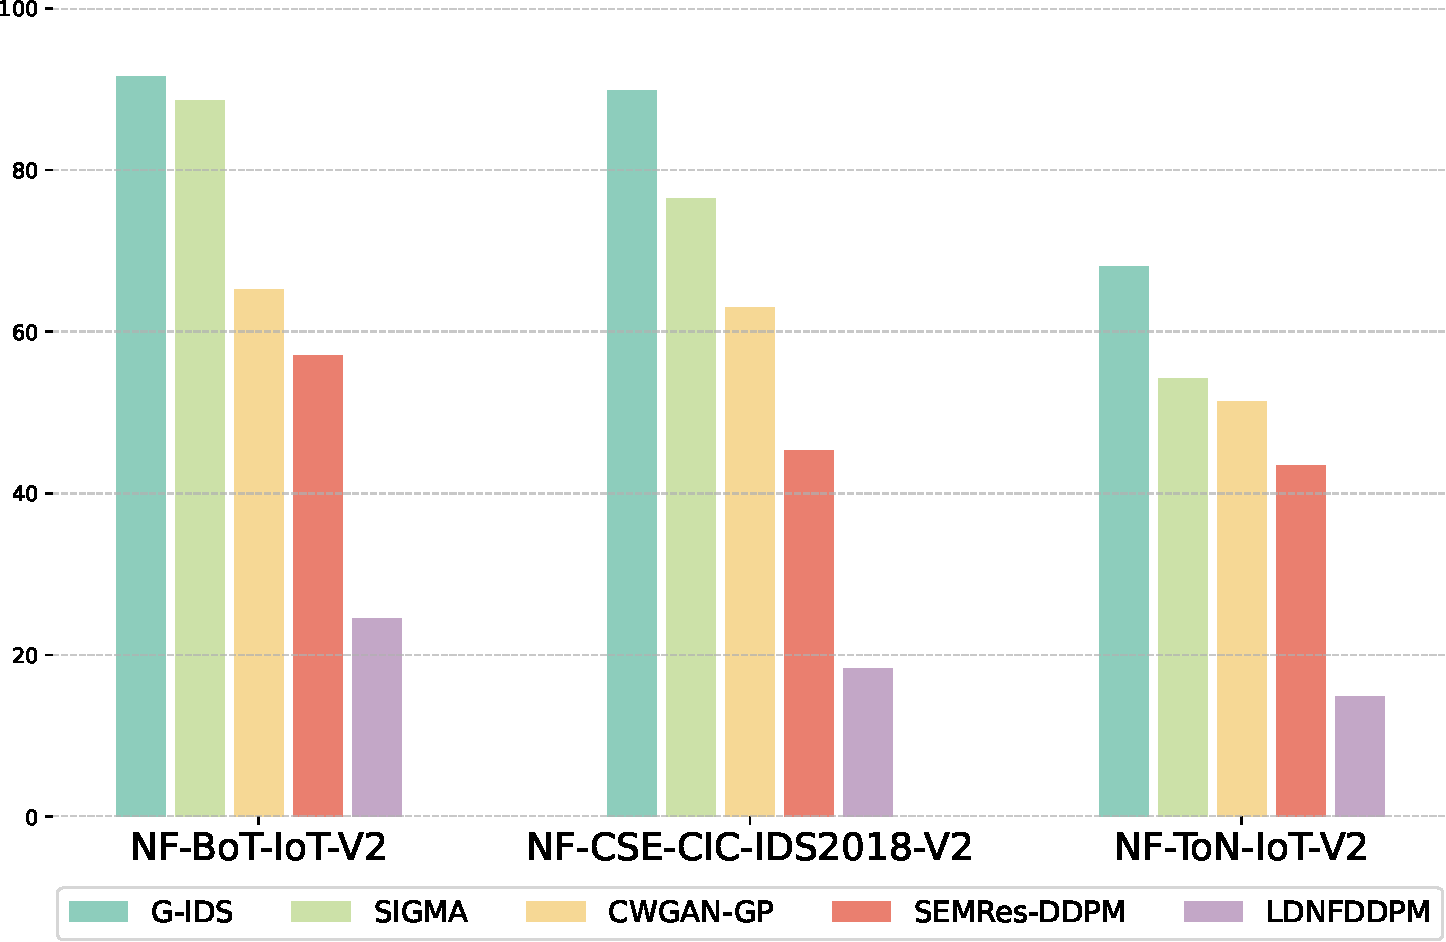
\includegraphics[width=1\linewidth]{./pic/chart1.pdf}
    \caption{不同方法数据增强的效果表现}
    \label{FID}
\end{figure}
(1)从整体来看,对于三个数据集上的FID表现来说,NF-BoT-IoT-V2略高于NF-CSE-CIC-IDS2018-V2,NF-CSE-CIC-IDS2018-V2略高于NF-ToN-IoT-V2。这是因为由于其攻击流量比例极高(99.64\%是攻击流量),且攻击类型较为简单,生成模型可能较容易生成攻击流量,但难以生成正常流量。虽然生成模型会聚焦于攻击流量的特征,但可能忽略了正常流量的多样性,这导致生成数据质量较低,FID 值较高。而NF-ToN-IoT-V2 良性流量比例相对较高(36.01\%),且该数据集包含多种协议(包括 IPv6-ICMP)。生成模型在生成攻击流量时的难度相对较大,但正常流量的特征较为明显,有助于生成模型较好地捕捉这些特征,因此 FID 值较低。对于NF-CSE-CIC-IDS2018-V2,该数据集复杂度最高,攻击类型多样,且协议种类丰富。生成模型在处理此类数据时需要学习到更复杂的特征,因此其 FID 处于两者之间。


(2)观察图\ref{FID}可知,G-IDS和SIGMA等基于传统GAN生成的数据,FID值较高,且在表\ref{MethodsOnNF-BoT-IoT-V2}至\ref{MethodsOnNF-ToN-IoT-V2_2}的性能指标中,识别率(Rec)较低,暗示这些生成数据与真实数据存在显著差异。这归因于传统GAN在有限样本上的学习局限,导致模型难以全面捕获特征并良好适应小数据集。优化后的 GAN(CWGAN-GP)在表\ref{MethodsOnNF-BoT-IoT-V2}和表\ref{MethodsOnNF-CSE-CIC-IDS2018-V2}中生成数据的检测的表现要优于 G-IDS,但图\ref{FID}中FID值仍然相对较高。这表明,在训练 GAN时引入条件信息指导生成器生成特定类别的样本在一定程度上可以提高 GAN 性能。

\begin{table}[h!]
\centering
\caption{NF-BoT-IoT-V2 数据集评估结果}
\begin{tabular}{c||cccccccc}
\hline\hline
\multirow{2}{*}{Method} & \multicolumn{2}{c}{DDoS} & \multicolumn{2}{c}{DoS} & \multicolumn{2}{c}{Reconnaissance} & \multicolumn{2}{c}{Theft} \\
                        & Pre         & Rec        & Pre        & Rec        & Pre              & Rec             & Pre         & Rec         \\ \hline
\textbf{LDNFDDPM}       & \textbf{93.68} & \textbf{89.47} & \textbf{92.01} & \textbf{86.45} & \textbf{88.56}     & \textbf{83.56}    & \textbf{59.12} & \textbf{60.34} \\\hline
G-IDS\citing{shahriar2020g}                   & 60.25       & 64.57      & 68.32      & 61.21      & 55.12            & 78.16           & 48.56       & 42.12       \\ \hline
SIGMA\citing{msika2019sigma}                    & 72.14       & 67.54      & 80.34      & 74.13      & 67.10            & 71.24           & 52.12       & 45.79       \\ \hline
CWGAN-GP\citing{kang2022cwgan}                 & 81.46       & 86.42      & 89.42      & 82.78      & 86.34            & 79.84           & 50.78       & 44.31       \\ \hline
SEMRes-DDPM\citing{zheng2024semres}                & 90.24       & 81.91      & 81.42      & 85.54      & 88.02            & 72.63           & 53.45       & 47.46       \\ 
\hline\hline
\end{tabular}
\label{MethodsOnNF-BoT-IoT-V2}
\end{table}
\begin{table}[h!]
\centering
\caption{NF-CSE-CIC-IDS2018-V2 数据集评估结果}
\resizebox{\textwidth}{!}{
\begin{tabular}{c||cccccccccc}
\hline\hline
\multirow{2}{*}{Method} & \multicolumn{2}{c}{DDos} & \multicolumn{2}{c}{Dos} & \multicolumn{2}{c}{Bot} & \multicolumn{2}{c}{BruteForce} & \multicolumn{2}{c}{Infiltration}                  \\
                        & Pre         & Rec        & Pre      & Rec          & Pre        & Rec        & Pre            & Rec           & \multicolumn{1}{c}{Pre} & \multicolumn{1}{c}{Rec} \\ \hline
\textbf{LDNFDDPM}       & \textbf{98.48} & \textbf{96.32} & \textbf{97.10} & \textbf{94.17} & \textbf{99.56} & \textbf{98.96} & \textbf{99.32} & \textbf{98.31} & \textbf{96.02} & \textbf{91.95} \\\hline
G-IDS\citing{shahriar2020g}                   & 66.42       & 62.18      & 54.72      & 59.01      & 68.05       & 55.14      & 77.98         & 64.98        & 63.56       & 66.23       \\ \hline
SIGMA\citing{msika2019sigma}                   & 77.58       & 74.63      & 76.12      & 62.28      & 68.78       & 67.11      & 78.64         & 66.67        & 74.98       & 79.48       \\ \hline
CWGAN-GP\citing{kang2022cwgan}                  & 77.10       & 73.67      & 75.68      & 71.42      & 78.42       & 76.32      & 78.28         & 75.84        & 64.45       & 68.56       \\ \hline
SEMRes-DDPM\citing{zheng2024semres}                & 88.05       & 93.56      & 91.78      & 93.54      & 92.14       & 88.24      & 89.02         & 90.59        & 94.68       & 91.24       \\ 
\hline\hline  

\end{tabular}
\label{MethodsOnNF-CSE-CIC-IDS2018-V2}
}
\end{table}
% Please add the following required packages to your document preamble:
% \usepackage{multirow}
\begin{table}[h!]
\centering
\caption{NF-ToN-IoT-V2 数据集评估结果}
\begin{tabular}{c||ccccccccc}
\hline\hline
\multirow{2}{*}{Method} & \multicolumn{2}{c}{DDoS} & \multicolumn{2}{c}{DoS} & \multicolumn{2}{c}{Backdoor} & \multicolumn{2}{c}{XSS} \\
                        & Pre         & Rec        & Pre        & Rec        & Pre           & Rec          & Pre        & Rec        \\ \hline
\textbf{LDNFDDPM}       & \textbf{94.68} & \textbf{91.47} & \textbf{92.12} & \textbf{88.42} & \textbf{98.56} & \textbf{97.28} & \textbf{86.34} & \textbf{81.23} \\\hline
G-IDS\citing{shahriar2020g}                    & 60.15       & 67.54      & 57.32      & 32.34      & 65.86         & 64.23        & 70.23      & 45.12      \\ \hline
SIGMA\citing{msika2019sigma}                   & 72.30       & 79.73      & 70.42      & 66.37      & 67.08         & 65.54        & 63.47      & 78.21      \\ \hline
CWGAN-GP\citing{kang2022cwgan}                  & 81.42       & 88.56      & 89.18      & 84.52      & 76.32         & 84.72        & 82.15      & 76.98      \\ \hline
SEMRes-DDPM\citing{zheng2024semres}                & 93.75       & 90.59      & 91.56      & 87.74      & 98.12         & 96.75        & 84.96      & 79.87      \\ 
\hline\hline
\end{tabular}
\label{MethodsOnNF-ToN-IoT-V2}
\end{table}
(3)与其他类型的数据增强方法相比,基于DDPM的方法(SEMRes-DDPM、LDNFDDPM)的FID值明显更低。这是因为DDPM通过逐步去噪的过程生成数据,避免了GAN中的模式崩溃和训练不稳定的问题,同时能够生成更加多样且高质量的样本。DDPM不依赖于生成器和判别器的对抗博弈,而是通过最大化数据似然进行训练,这使得它在数据稀缺或复杂分布的情况下表现得更加鲁棒和可靠。相较于SEMRes-DDPM,LDNFDDPM展现出了更优的性能,体现在较低的FID值和在同类数据集上更高的识别率。这得益于它专注于生成非功能特征,同时通过加重游离IP的权重,增强了样本的真实感并简化了训练过程。







% Please add the following required packages to your document preamble:
% \usepackage{multirow}
\begin{table}[h!]
\centering
\caption{NF-ToN-IoT-V2 数据集评估结果(续表)}
\begin{tabular}{c||cccccc}
\hline\hline
\multirow{2}{*}{Method} & \multicolumn{2}{c}{Scanning} & \multicolumn{2}{c}{Injection} & \multicolumn{2}{c}{Password} \\
                        & Pre        & Rec        & Pre        & Rec        & Pre           & Rec          \\ \hline
\textbf{LDNFDDPM}       & \textbf{97.01} & \textbf{93.56} & \textbf{85.01} & \textbf{87.65} & \textbf{76.43} & \textbf{69.12} \\ \hline
G-IDS\citing{shahriar2020g}                   & 63.45      & 59.17      & 69.56      & 53.52      & 60.58         & 63.12        \\ \hline
SIGMA\citing{msika2019sigma}                   & 65.02      & 61.28      & 61.25      & 65.56      & 73.85         & 66.14        \\ \hline
CWGAN-GP\citing{kang2022cwgan}                  & 74.12      & 79.94      & 80.34      & 84.35      & 72.42         & 64.71        \\ \hline
SEMRes-DDPM\citing{zheng2024semres}                & 96.23      & 92.85      & 92.45      & 87.08      & 75.12         & 67.85        \\ 
\hline\hline
\end{tabular}
\label{MethodsOnNF-ToN-IoT-V2_2}
\end{table}

2.消融实验

此次实验的主要目的是测试划分功能/非功能特征以及关注游离IP行为对于数据增强效果的影响以及滑动窗口和重叠率设计对入侵检测性能的影响。

为了深入探讨非功能特征和游离IP行为对于数据增强效果的影响,本节基于LDNFDDPM设计了两种变体:LDDDPM、NFDDPM。

LDDDPM:不对特征进行功能性、非功能性划分,直接进行加噪去噪过程。

NFDDPM:不对游离IP做额外处理。



% Please add the following required packages to your document preamble:
% \usepackage{multirow}
\begin{table}[h!]
\centering
\caption{不同消融设置下的数据增强表现}
\begin{tabular}{c||ccc}
\hline\hline
\multirow{2}{*}{Method} & \multicolumn{3}{c}{FID}                               \\
                        & NF-BoT-IoT-V2 & NF-CSE-CIC-IDS2018-V2 & NF-ToN-IoT-V2 \\ \hline
\textbf{LDNFDDPM}                & \textbf{24.50}         & \textbf{18.30}                 & \textbf{14.90}        \\\hline
LDDDPM                  & 47.15         & 41.54                 & 37.32         \\ \hline
NFDDPM                  & 46.28         & 42.56                 & 34.17         \\
\hline\hline
\end{tabular}
\label{Data_augmentation_based_on_ablation}
\end{table}

各变体在不同数据集上的实验结果如表\ref{Data_augmentation_based_on_ablation}所示,可以看出,LDNFDDPM的FID值要低于LDDDPM,这表明,LDNFDDPM通过保存数据功能性特征,有助于生成模拟数据。同样,LDNFDDPM的FID值要低于NFDDPM,这表明,关注游离IP,对生成数据的真实性有一定提升。此外,在数据集NF-ToN-IoT-V2上NFDDPM的FID值要小于LDDDPM,这是因为NF-ToN-IoT-V2数据集的游离IP偏多,这也恰恰说明针对游离IP进行权重提升能够提高生成数据的真实性。


为了深入探讨滑动窗口和重叠率设计对入侵检测性能的影响,本实验去除了滑动窗口机制中的重叠率,即完全使用不重叠的窗口进行图快照切割,并观察在没有滑动窗口重叠的情况下,模型的检测性能变化。
具体而言,网络流量数据被按时间戳切割成多个图快照,每个快照仅代表某个特定的时间段,且相邻的快照之间没有重叠部分。在此框架下,模型仅依赖于这些不重叠的图快照中的网络拓扑信息进行训练。

如表\ref{table:ablation_window_overlap}所示,当没有滑动窗口重叠(重叠率为0)时,模型的准确率(ACC)和F1分数显著下降。这表明,当没有滑动窗口机制的支持时,网络流量的动态演变信息未能得到有效捕捉,导致模型在处理长时间序列时表现不佳。
特别是,在较长的时间序列中,网络流量的突发性变化无法通过单一的图快照反映出来,从而影响了检测性能。

进一步地,在使用不同重叠率(0、0.3、0.5、0.9)的滑动窗口机制进行实验时,结果显示随着重叠率的增加,模型的性能逐步提升。具体来说,当重叠率为0.3、0.5、0.9时,模型的ACC分别为0.9264、0.9311、0.9466,F1分数也随之增加。
此实验结果表明,滑动窗口的重叠率有助于捕捉到更丰富的时序信息,提升了模型在长时间序列中的稳定性和检测精度。

此外,随着滑动窗口重叠率的增加,模型的准确率方差从0.017下降至0.014,这进一步证明了滑动窗口机制能够提高模型在长时间序列场景中的数值稳定性。总体而言,滑动窗口和重叠率设计在捕捉网络流量的长期依赖性和时序变化方面发挥了重要作用,
尤其在面对网络攻击的长期演化过程中,能够显著提升检测性能。
\begin{table}[h!]
    \centering
    \caption{滑动窗口与重叠率设计的消融实验结果}
    \label{table:ablation_window_overlap}
    \begin{tabular}{c||ccc}
    \hline
    \textbf{重叠率} & \textbf{准确率 (ACC)} & \textbf{F1分数} & \textbf{准确率方差} \\ \hline
    0.0             & 0.9203               & 0.9102          & 0.017             \\ \hline
    0.3             & 0.9264               & 0.9155          & 0.016             \\ \hline
    0.5             & 0.9311               & 0.9198          & 0.015             \\ \hline
    0.9             & 0.9466               & 0.9273          & 0.014             \\ \hline
    \end{tabular}
\end{table}

\section{本章小结}
本章提出了一种基于LDNFDDPM的数据增强方法,旨在解决恶意流量检测中的数据不平衡问题。通过对流量数据进行清洗、标签转换、特征提取和标准化处理,结合低度IP节点的增强策略和功能性、
非功能性特征的划分,提出了一个改进的去噪扩散概率模型。该模型通过引入时序图捕捉流量数据的时间依赖性,增强了对稀有攻击类型和低度IP节点的生成能力,
从而提高了模型的鲁棒性和生成样本的质量,为网络流量检测提供了更为有效的数据增强方案。通过在多个数据集上的实验,验证了该方法的有效性。

\chapter{基于线图的恶意流量检测方法 }
本章提出了一种基于线图的恶意流量检测方法(Line Graph-based Malicious Traffic Detection,LG-MTD)。首先,利用第三章提出的数据增强技术对离线
训练数据进行处理,并采用线图结构来更有效地捕捉边的特征,从而提升模型的表达能力。接着,引入自适应多头注意力机制,
在图神经网络中通过动态调整节点间的注意力权重,实现更精确的消息传递和特征聚合。这一机制帮助模型更好地捕捉节点间的复杂关系,
进一步增强其表达能力。最后,采用MAD指标,评估数据集中各个数据点与其均值之间的偏差,分析图神经网络在不同层次上的特征分布变化,
尤其是邻居节点和远程节点之间的特征差异。通过在多个数据集上进行广泛严谨实验,证明了与最先进的方法相比,提出的方法效果显著提升。
\section{问题描述和研究思路}
图神经网络现广泛应用于多个领域,如社交分析、推荐、化学建模和网络安全,因其在处理图结构数据方面的卓越能力。图结构数据的独特性使得传统的深度学习方法(如卷积神经网络、循环神经网络等)难以直接应用,从而推动了图神经网络的发展。图神经网络通过消息传递机制,使节点能够根据图的拓扑结构和节点特征与邻居节点交换信息,从而逐层更新节点的表示。这种机制对于大多数图数据任务,如节点分类、图分类和链接预测等,表现出了较强的能力。

然而,随着图数据的复杂性逐步增加,尤其是当图结构规模扩大或者图中的节点和边表现出更复杂的关系时,现有的图神经网络方法常常面临一系列挑战。首先,图中节点间的关系并非是静态且均匀的。在实际应用中,图结构往往包含多种类型的边,且不同的边在图中对节点的影响和重要性有所不同。许多传统的图神经网络方法通常通过固定的消息传递规则,假定所有边对节点的影响是相等的,这使得它们难以捕捉图中复杂的边的特征和节点之间的不同关系。

此外,节点间的关系不仅仅是邻近节点的作用,图中的远程节点之间也可能存在潜在的联系。这些远程节点的特征可能对于节点的表示至关重要,但在传统的图神经网络中,随着图的层次加深,远程节点的影响会逐渐被忽视,导致模型无法有效地捕捉长距离的依赖关系。为了克服这一问题,通常需要更为复杂的网络架构和更精细的信息传播策略。

再者,现有的图神经网络方法往往依赖于图的邻接矩阵或边列表来表示图结构,但这也意味着图的边的特征简单地表示为固定的权重或标签,未能充分利用边之间的高阶关系。传统的图神经网络方法通常聚焦于节点的邻居信息,并在每一层将节点特征与邻居节点的特征进行聚合,但这一过程忽略了边与边之间的潜在复杂关系,限制了模型的表达能力。

这些问题表明,现有的图神经网络方法存在一些局限性,需要新的方法来更好地捕捉节点和边之间的复杂关系,尤其是在节点间关系动态变化的情况下。因此,如何优化图神经网络中的消息传递机制,提高模型对边特征的敏感度,以及如何改进远程节点之间信息的传递与融合,成为了提升图神经网络性能的关键问题。本章提出了一种基于线图的恶意流量检测方法,旨在通过创新的结构与机制来克服现有方法的局限,从而优化图神经网络的性能。


LG-MTD总体结构图如图\ref{lineAndAttention}所示,首先,在扩充的图数据集基础上,构建了线图结构。线图结构能够更好地捕捉图中节点之间的关系,从而提高模型的表达能力。通过将原始图转换为线图,能够更细致地分析节点之间的交互关系,这对于复杂网络数据的处理尤为重要。

\begin{figure}[h!]
    \centering
    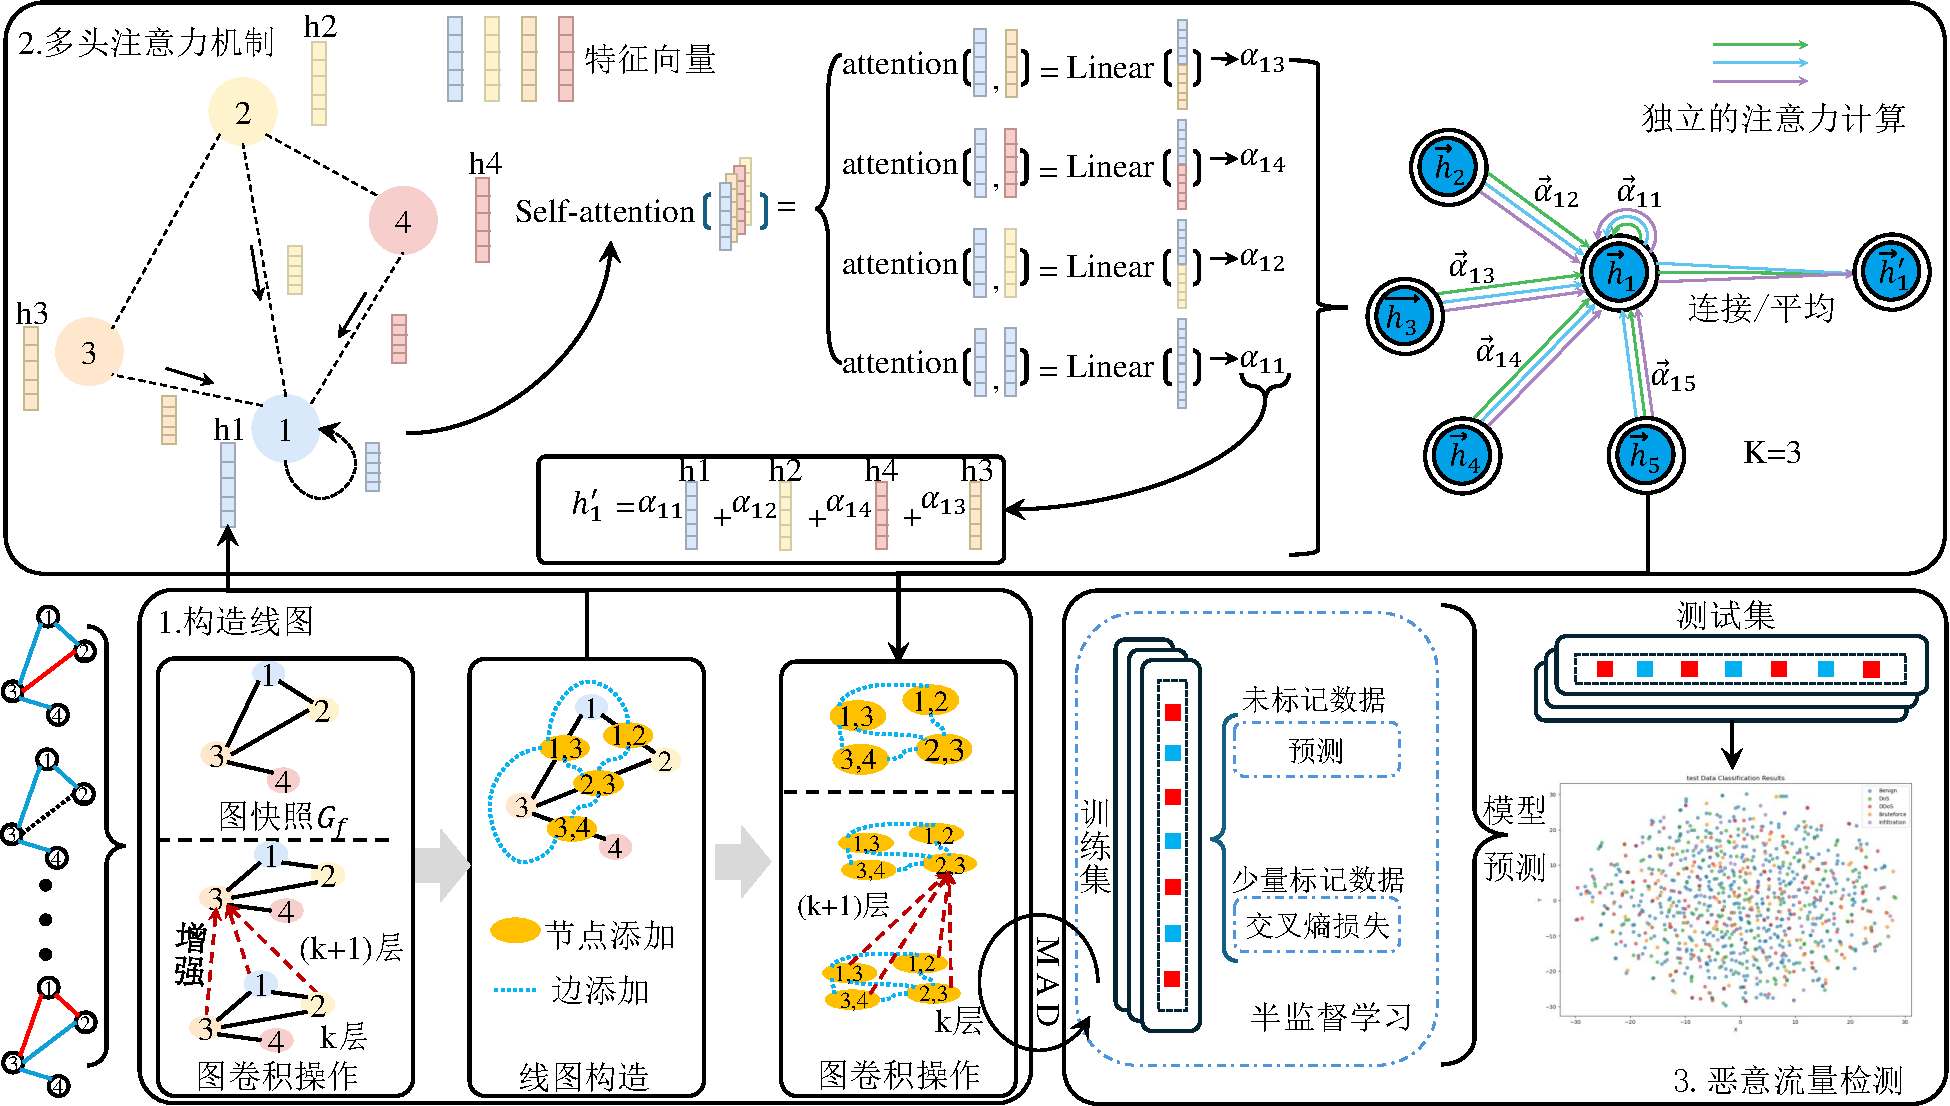
\includegraphics[width=1\linewidth]{./pic/线图+多头注意力(大字版).pdf}
    \caption{基于多头自适应注意力机制的线图训练模型}
    \label{lineAndAttention}
\end{figure}

然后,引入了多头注意力机制。多头注意力机制通过同时关注图中不同部分的信息,能够更有效地捕捉复杂的图结构特征,提高模型的分类性能。具体来说,多头注意力机制允许模型在不同的子空间中独立地学习节点之间的关系,从而增强模型的表达能力和鲁棒性。

为了进一步提升模型的性能,还引入了 MAD-GAP 正则化器(MAD-GAP Regularizer)。MAD-GAP 正则化器通过在训练过程中对注意力权重进行正则化,能够有效防止模型过拟合,并提高模型的泛化能力。具体来说,MAD-GAP 正则化器通过在注意力权重上施加约束,防止模型过度依赖某些特定的节点或边,从而增强模型的鲁棒性和稳定性。

在此基础上,构建了一个半监督学习模型。半监督学习能够利用少量标注数据和大量未标注数据进行训练,从而在标注数据有限的情况下仍能取得较好的分类效果。通过结合有监督和无监督学习的优势,半监督学习模型能够更好地利用数据中的信息,提高分类的准确性和泛化能力。

\section{框架设计}
\subsection{基于LineGraph的特征结合 }
为了更有效地分析网络流量中的复杂交互关系,本研究采用线图(Line Graph)作为分析工具。线图能够将原始图中的边转换为新图中的节点,并在这些节点之间建立连接,以反映原始图中边的相互关系。这种方法在检测网络攻击和异常流量时具有显著优势。

线图在恶意流量检测中的作用体现在以下几个方面。首先,在网络攻击中,攻击流量往往通过多个源IP发起,边与边之间可能存在复杂的交互。线图将原图中的边转化为节点,捕捉边与边之间的共享节点关系。例如,DDoS攻击中多个源IP向同一目标IP发起流量,线图能够有效捕捉这些攻击源之间的高阶依赖关系。

其次,线图将原图中的边特征映射为新节点特征,从而加强了对边特征的学习。举例来说,Brute Force攻击可能通过特定端口发起,而正常流量则有不同的协议和端口分布,线图能够识别这些特征并提高检测精度。

此外,恶意流量可能跨越多个路径,导致攻击源与目标之间的关系较远。线图增强了对远程节点间关系的建模能力,能够识别例如DDoS攻击中分布式流量的协调行为。

线图还能够帮助识别潜在的攻击模式,尤其是当恶意流量依赖于多次交互模式时。例如,持续的流量模式可能通过多次交互形成攻击特征,线图帮助识别这些复杂模式。

最后,恶意流量常常表现为低频或隐蔽的异常行为,线图通过聚合边间的关系,提高了图神经网络在处理这些稀疏数据时的鲁棒性。线图可以帮助识别出在常规流量中难以察觉的低频攻击。

线图 \( L(G) \) 是从原始图 \( G = (V, E) \) 构建而来的,其中 \( V \) 是节点集合,\( E \) 是边集合。在线图中,节点集合 \( V' \) 对应于原始图中的边集合 \( E \),即:
\begin{equation}
V' = \{ e_i \mid e_i \in E \}
\end{equation}

对于任意两条边 \( e_i, e_j \in E \),如果它们在原始图中共享一个公共节点,则在线图中添加一条边 \( (e_i, e_j) \)。这种边的添加可以通过以下方式表示:
\begin{equation}
E' = \{ (e_i, e_j) \mid e_i \cap e_j \neq \emptyset \}
\end{equation}

在该公式中, \( e_i \cap e_j \) 表示边 \( e_i \) 和 \( e_j \) 之间的公共节点。通过这种转换,线图能够将原图中的边之间的关系转化为节点之间的连接,从而揭示流量之间的复杂交互关系,转换过程如图\ref{lineGraph_transport}所示。

在线图 \( L(G) \) 中,原始图 \( G \) 的每条边 \( e = (u, v) \) 被转化为线图中的一个节点。因此,需要为线图中的新节点设计特征,以保留原始图中边的丰富语义信息。

在本研究中,我们采用以下策略进行节点特征构建:

\begin{itemize}
    \item 边特征映射: 由于原始网络流量图中,每条边通常携带丰富的流量统计特征(如包字节数、持续时间、TTL值、重传次数等),我们直接将每条边的特征作为线图中新节点的初始特征向量。设原图中第 \(i\) 条边的特征为 \( \mathbf{f}_i \),则在线图中对应节点 \(v'_i\) 的特征为 \( \mathbf{x}'_i = \mathbf{f}_i \)。
    
    \item 节点特征融合: 为进一步增强特征表达能力,我们还可以将原始边的两端节点(即源节点 \(u\) 和目标节点 \(v\))的特征进行拼接或融合,作为补充信息。具体来说,若原节点特征为 \( \mathbf{h}_u \) 和 \( \mathbf{h}_v \),则线图节点特征可以构建为:
    \begin{equation}
         x'_i = \text{Concat}(f_i, h_u, h_v)
    \end{equation}
    或采用加权求和、注意力融合等方式整合节点特征和边特征。
    
    \item 归一化处理: 为避免不同特征尺度差异对训练造成不利影响,我们在特征结合后对所有特征进行归一化处理,如采用标准化(Z-Score)或归一到 [0,1] 区间。
\end{itemize}

通过以上特征构建策略,线图不仅能够保留原始边的关键信息,还能进一步引入节点级上下文信息,从而提升后续图神经网络在恶意流量检测任务中的建模能力。

\begin{figure}[h!]
    \centering
    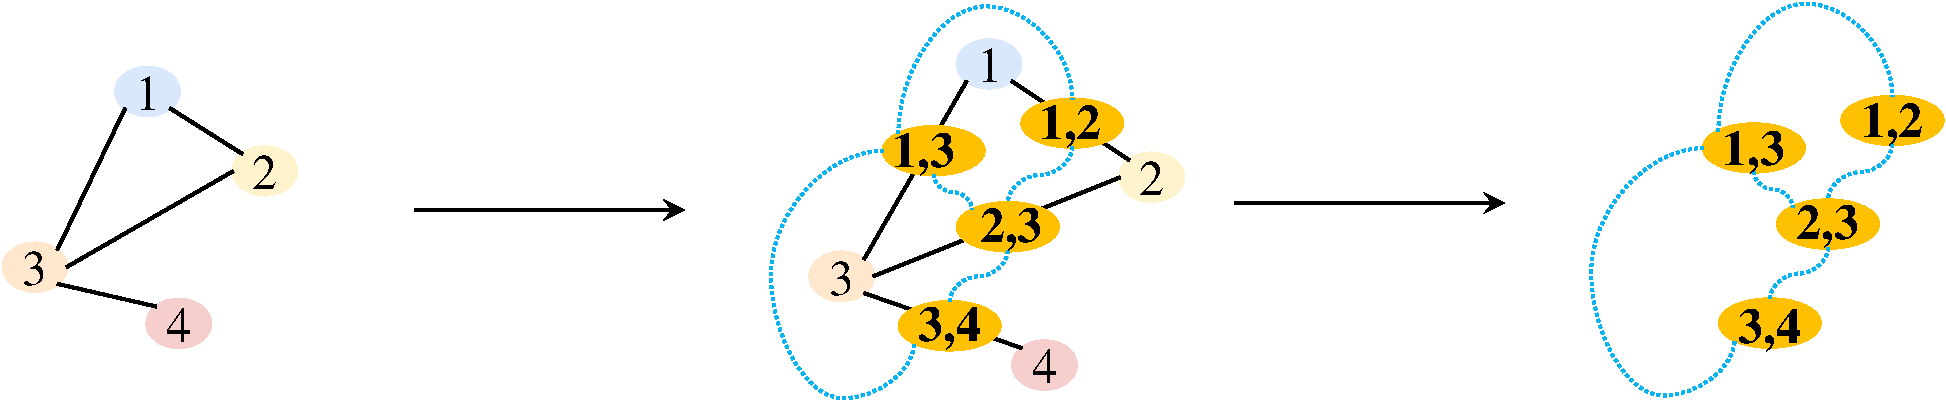
\includegraphics[width=1\linewidth]{./pic/线图转换.pdf}
    \caption{线图转换过程}
    \label{lineGraph_transport}
\end{figure}
\begin{algorithm}[h!]
    \caption{融合节点特征的原图转线图算法}
    \label{transformLineGraphWithFeature}
    \KwIn{原始图 $G = (V, E, F_V, F_E)$,其中 $V$ 是节点集合,$E$ 是边集合,$F_V$ 是节点特征集合,$F_E$ 是边特征集合}
    \KwOut{线图 $L(G) = (V', E', F_{V'})$,其中 $V'$ 是线图节点集合,$E'$ 是线图边集合,$F_{V'}$ 是线图节点特征集合}
    
    $L(G) \gets$ 空图\;
    \ForEach{边 $e = (u, v) \in E$}{
        在 $L(G)$ 中添加一个节点 $e$\;
        将节点 $e$ 的特征设置为 $f_e' = \texttt{Fuse}(F_V(u), F_V(v), F_E(e))$\;
    }
    
    \ForEach{一对边 $e_1 = (u_1, v_1)$ 和 $e_2 = (u_2, v_2)$}{
        \If{$v_1 = u_2$ 或 $u_1 = v_2$ 或 $u_1 = u_2$ 或 $v_1 = v_2$}{
            在 $L(G)$ 中添加一条边 $(e_1, e_2)$\;
        }
    }
    
    \Return{$L(G)$}\;
    \end{algorithm}
    
    
在构建线图时,每条边 $e = (u, v)$ 成为线图中的一个节点。然后,对于原始图中相邻的两条边(即它们在一个共享的节点处相连),
在 $L(G)$ 中添加一条连接它们的边。算法通过遍历原始图中的每条边,首先为每条边在 $L(G)$ 中添加节点,再根据边的相邻关系在 $L(G)$ 中添加边,
最终返回构建好的线图 $L(G)$。详细的线图转换算法如算法\ref{transformLineGraphWithFeature}所示。


\subsection{基于多头自适应注意力机制的图卷积}
在线图转换后,由于节点和边的数量急剧增加,如图\ref{largeLine}所示。传统的图神经网络面临着巨大的计算资源压力。在这种情况下,为了提高训练效率和模型的表达能力,结合多头注意力机制和中位数绝对偏差(MAD)正则化提供了一个有效的解决方案。多头注意力机制能够有效捕捉节点间的复杂依赖关系,而MAD正则化则能够抑制特征间的噪声,提升信息传递的稳定性。两者的结合不仅缓解了计算负担,还增强了模型的鲁棒性和表达能力。
\begin{figure}[h!]
    \centering
    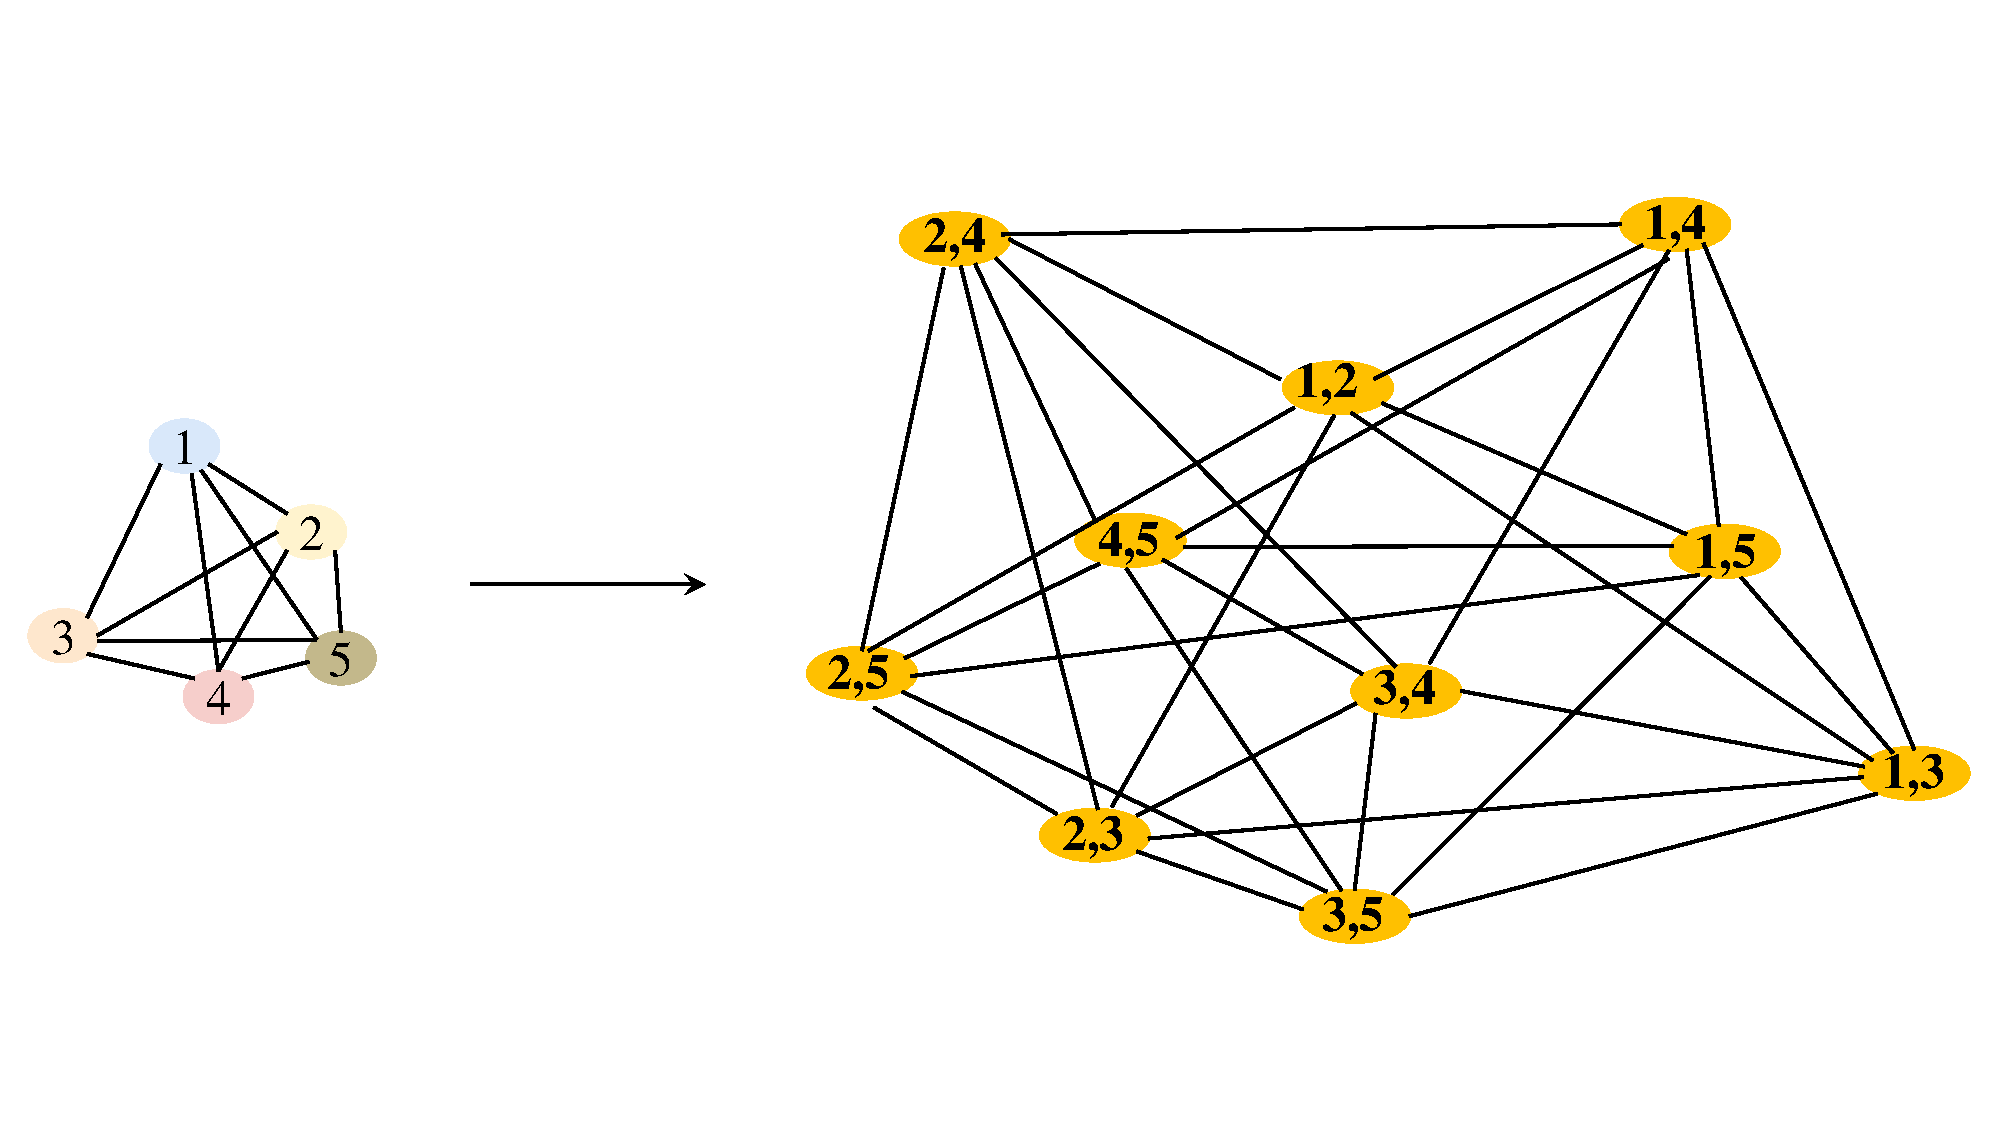
\includegraphics[width=1\linewidth]{./pic/线图转换维度增加.pdf}
    \caption{线图转换规模增加}
    \label{largeLine}
\end{figure}

多头注意力机制通过并行计算多个注意力头,分别学习不同的特征子空间,并将这些子空间的结果进行拼接,最终生成更加丰富的节点表示。在图神经网络中,多头注意力可以用来动态调整节点之间的信息传递强度。每个注意力头能够独立地关注不同的邻居节点,学习到不同的依赖关系,这使得信息传递变得更加多样化,从而增强了模型的表达能力。

具体地,多头注意力的计算可以通过以下公式表示:
\begin{equation}
\text{MultiHead}(\mathbf{h}) = \text{Concat}\left( \text{head}_1, \dots, \text{head}_K \right) \mathbf{W}^O
\end{equation}

其中,\(\text{head}_i = \text{Attention}(\mathbf{h})\) 是第 \(i\) 个注意力头的输出,\(K\) 是注意力头的数量,\(\mathbf{W}^O\) 是输出的线性变换矩阵。每个注意力头通过自注意力机制计算节点间的相关性,然后将这些输出拼接起来,进一步通过线性变换生成最终的节点表示。

多头注意力机制可以有效减少冗余计算,并且能够从多个角度捕捉图的结构信息。这在处理大规模线图时尤为重要,因为多个注意力头可以并行计算,减轻了计算负担并提高了模型的学习能力。

然而,尽管多头注意力机制能够有效捕捉多样化的节点特征,在线图中,由于节点特征之间的差异较大,信息传递过程中可能会存在较大的噪声,尤其是在处理具有高复杂度的图时。这种噪声会导致节点特征的过度偏移,进而影响模型的收敛性和最终性能。为了减少这种影响,结合MAD正则化是一种有效的策略。

MAD(Mean Absolute Deviation)是一种衡量数据离散程度的统计量,能够有效地约束节点特征在信息传播过程中的偏差。在节点特征的聚合过程中,MAD通过计算特征的离散程度,动态调整每个节点的权重,确保特征传播更加稳定。具体地,MAD的计算方式为:
\begin{equation}
\text{MAD}(x) = \frac{1}{n} \sum_{i=1}^{n} \left| x_i - \mu \right|
\end{equation}
其中,\( x_i \) 是节点 \( i \) 的特征,\(\mu\) 是节点特征的均值,\(n\) 是节点数。

需要注意的是,虽然MAD能够有效衡量节点特征的离散程度,但在图结构中直接应用MAD存在一定局限性。由于图中节点之间存在复杂的语义关系(例如邻居节点通常特征相似,而远程节点特征差异较大),单纯基于特征值计算离散度,可能混淆了局部一致性和全局异质性。此外,图中不同区域的节点密度差异较大,特征尺度不同,直接计算MAD可能放大稀疏区域的噪声,削弱密集区域的信息。

针对上述问题,本研究在引入MAD正则化时,进一步限制MAD的计算范围,仅基于节点的直接邻居集合进行局部特征偏差估计,从而避免远程节点特征差异带来的偏移。同时,为了缓解节点度差异的影响,引入归一化处理,使得不同节点在特征传播过程中的影响更加平衡。局部MAD的计算公式如下:
\begin{equation}
\text{MAD}_{\text{local}}(i) = \frac{1}{|\mathcal{N}(i)|} \sum_{j \in \mathcal{N}(i)} \left| h_j - \bar{h}_{\mathcal{N}(i)} \right|
\end{equation}
其中,\(\mathcal{N}(i)\) 表示节点 \(i\) 的邻居节点集合,\(\bar{h}_{\mathcal{N}(i)}\) 为邻居节点特征的均值。

结合多头注意力机制与局部MAD正则化,可以在计算复杂图结构时有效减少噪声带来的负面影响,并提升模型的鲁棒性。多头注意力机制通过并行处理多个不同的注意力视角,能够捕捉到节点特征之间的多样化依赖关系;而局部MAD正则化通过在局部范围内约束特征的离散程度,抑制了噪声的扩散,确保信息传递更加稳定和精确。

具体来说,节点特征的更新公式可以表示为:
\begin{equation}
h_i' = \sigma \left( \sum_{j \in \mathcal{N}(i)} \frac{ \mathbf{A}_{ij} h_j}{d_j} + \beta \cdot \text{MAD}_{\text{local}}(i) \right)
\end{equation}
其中,\( h_i \) 是节点 \(i\) 的特征,\( \mathcal{N}(i) \) 是节点 \(i\) 的邻居节点集合,\(\mathbf{A}_{ij}\) 表示节点 \(i\) 和节点 \(j\) 之间的邻接矩阵元素,\(d_j\) 是节点 \(j\) 的度数,\(\beta\) 是用于调节局部MAD正则化项影响的超参数。

通过这种结合,多头注意力机制能够在处理大规模图时并行捕捉多样化依赖关系,而局部MAD正则化则帮助减少特征差异带来的噪声干扰,增强信息传递的稳定性。这种方法不仅提高了计算效率,还提升了模型对复杂图结构的表达能力和泛化能力。
在线图转换后的节点数和边数急剧增加,带来了计算资源的挑战。结合多头注意力机制和MAD正则化,不仅能够减轻计算负担,还能有效提升模型的鲁棒性和表达能力。多头注意力机制通过并行计算多个注意力头,捕捉不同的节点依赖关系,增强了图的表达能力;而MAD正则化则通过约束节点特征的离散度,抑制了噪声的影响,确保了信息传递的精度和稳定性。两者的结合提供了一种有效的解决方案,使得图神经网络在处理大规模、复杂图数据时能够高效地进行训练,并且具有较强的泛化能力。
\subsection{基于半监督学习的模型训练}

在恶意流量检测任务中,数据的标注工作往往需要大量的人工干预,导致标注数据的获取成本高昂。为了有效利用未标注的数据,并在有限的标注数据上获得良好的检测性能,半监督学习方法成为一种非常有效的策略。半监督学习利用了大量未标注的数据,并结合少量标注数据,通过学习数据的潜在结构,提升模型的学习能力。在本研究中,基于图神经网络的恶意流量检测任务中,半监督学习尤其重要,因为图数据通常包含大量的节点和边,而边的标注往往稀缺,因此有效的划分数据集并利用未标注数据进行训练至关重要。

上一小节引入了MAD用于评估每个节点的特征偏差,调整节点权重。在数据集划分的过程中,将MAD与余弦相似度结合使用,能够进一步提升数据划分的有效性。

首先,通过计算数据点之间的余弦相似度,如公式\ref{cos}所示,我们能够将相似的数据点聚集到同一簇中,确保每个簇内的数据点特征较为相似。
\begin{equation}
\text{sim}(d_i, d_j) = \frac{\mathbf{x}_i \cdot \mathbf{x}_j}{\|\mathbf{x}_i\| \|\mathbf{x}_j\|}
\label{cos}
\end{equation}
其中,$\mathbf{x}_i$ 和 $\mathbf{x}_j$ 是数据点 $d_i$ 和 $d_j$ 的特征向量,$\cdot$ 表示向量的点积,$\|\mathbf{x}_i\|$ 和 $\|\mathbf{x}_j\|$ 分别表示它们的模长。

其中,$D$ 是数据集,$\bar{x}$ 是数据集 $D$ 的均值,$x_i$ 是第 $i$ 个数据点的特征。


\begin{algorithm}[h!]
\SetAlgoLined
\KwIn{数据集 $D = \{d_1, d_2, \dots, d_n\}$,每个数据点的特征向量 $\mathbf{x}_i$}
\KwOut{训练集 $D_{\text{train}}$,测试集 $D_{\text{test}}$}

\textbf{Step 1:} 计算余弦相似度矩阵 $S$:\;
\For{$i = 1$ \KwTo $n$}{
    \For{$j = 1$ \KwTo $n$}{
        计算 $\text{sim}(d_i, d_j)$ 并存储相似度值 $S_{ij}$\;
    }
}

\textbf{Step 2:} 使用K-means对相似度矩阵 $S$ 进行聚类,得到簇 $C_1, C_2, \dots, C_k$。

\textbf{Step 3:} 计算每个簇的 MAD 值:\;
\For{$k = 1$ \KwTo $k$}{
    计算簇 $C_k$ 的 MAD 值:$\text{MAD}(C_k) = \frac{1}{|C_k|} \sum_{i \in C_k} |x_i - \bar{x}_{C_k}|$\;
}

\textbf{Step 4:} 基于 MAD 值调整划分:\;
\For{$k = 1$ \KwTo $k$}{
    \If{MAD$(C_k)$ 较大}{
        将偏差较大的数据点重新划分到其他簇中\;
    }
}

\textbf{Step 5:} 划分训练集和测试集:\;
从每个簇中随机选取 70\% 的数据为训练集,剩余 30\% 为测试集\;
\caption{基于余弦相似度和 MAD 的数据划分算法}
\label{devidedData}
\end{algorithm}
基于余弦相似度计算得到的相似度矩阵可以用于将相似的数据点划分到同一个簇中。然而,在图数据中,单纯基于相似度进行划分可能导致数据分布不均匀,从而影响后续的训练效果。因此,引入MAD指标来评估每个簇内节点的特征分布偏差,MAD值较大的簇表示该簇的特征分布较为离散,从而可以进一步调整数据划分,将特征偏差较大的数据点重新划分到其他簇中。如公式\ref{MAD-equation}所示:
\begin{equation}
\text{MAD}(D) = \frac{1}{n} \sum_{i=1}^{n} |x_i - \bar{x}|
\label{MAD-equation}
\end{equation}

基于余弦相似度和MAD结合的划分过程如算法\ref{devidedData}所示,算法 1 至 5 行:计算数据点之间的余弦相似度矩阵。算法 6 至 8 行:使用 K-means 聚类算法对相似度矩阵进行聚类,得到簇。算法 9 至 11 行:计算每个簇的 MAD 值,评估特征分布偏差。算法 12 至 16 行:根据 MAD 值调整数据划分,重新分配特征偏差较大的数据点。


\section{实验分析}
本章实验所用到的实验设置与实验数据同第三章一致,用以验证所提出的模型在恶意流量检测任务中的有效性。
\subsection{评估指标}

混淆矩阵用于分类任务中,表示模型在不同类别上的预测结果。通过混淆矩阵可以计算多个关键指标,包括准确率、精确率、召回率和F1-Score等。二分类任务中的混淆矩阵结构如表\ref{ConfusionMatrix}所示:

\begin{table}[h!]
    \caption{混淆矩阵}
    \begin{tabular}{c||c c}
    \hline\hline
    \textbf{} & \textbf{预测为正类} & \textbf{预测为负类} \\
    \hline
    真实为正类 & \text{TP (True Positive)} & \text{FN (False Negative)} \\\hline
    
    真实为负类 & \text{FP (False Positive)} & \text{TN (True Negative)} \\
    \hline\hline
    \end{tabular}
    \label{ConfusionMatrix}
\end{table}

其中:
TP:真正例,表示模型正确地将正类样本分类为正类。
FP:假正例,表示模型错误地将负类样本分类为正类。
TN:真负例,表示模型正确地将负类样本分类为负类。
FN:假负例,表示模型错误地将正类样本分类为负类。


(1)准确率 (Accuracy)

准确率指模型正确分类的样本数与总样本数之比,计算公式如\ref{Acc}所示:
\begin{equation}
\text{Accuracy} = \frac{TP + TN}{TP + TN + FP + FN}
\label{Acc}
\end{equation}

(2)精确率 (Precision)

精确率是指在所有被模型预测为正类的样本中,实际上确实是正类的比例,计算公式如\ref{Pre}所示:
\begin{equation}
\text{Precision} = \frac{TP}{TP + FP}
\label{Pre}
\end{equation}

(3)召回率 (Recall)

召回率指的是在所有实际为正类的样本中,模型正确预测为正类的比例,计算公式如\ref{Rec}所示:
\begin{equation}
\text{Recall} = \frac{TP}{TP + FN}
\label{Rec}
\end{equation}

(4)F1-Score

F1-Score是精确率和召回率的调和平均数,计算公式如\ref{F1}所示:
\begin{equation}
F1 = 2 \times \frac{\text{Precision} \times \text{Recall}}{\text{Precision} + \text{Recall}} = 2 \times \frac{TP}{2TP + FP + FN}
\label{F1}
\end{equation}

(5)误报率 (False Positive Rate)

误报率衡量的是所有负类样本中,模型错误预测为正类的比例,计算公式如\ref{FPR}所示:
\begin{equation}
\text{False Positive Rate (FPR)} = \frac{FP}{FP + TN}
\label{FPR}
\end{equation}

\subsection{相关对比方法}
为了评估LG-MTD在恶意流量方面的检测性能,选取了现有的几种物联网恶意流量检测方法进行比较,具体如表\ref{detectMethods}所示:



\begin{table}[h!]
\centering
\caption{恶意流量检测方法对比}
\resizebox{\textwidth}{!}{
\begin{tabular}{c||>{\centering\arraybackslash}p{0.33\linewidth}>{\centering\arraybackslash}p{0.4\linewidth}}  % 设置列宽
\hline\hline
\textbf{方法} & \textbf{描述} & \textbf{优缺点} \\
\hline
E-GraphSAGE \citing{lo2022graphsage} & 基于图神经网络,捕捉边特征和拓扑信息。 &  适用于图结构数据,但对大数据处理复杂。 \\
\hline
Extra Trees \citing{sarhan2021netflow} &  基于决策树的集成学习方法,构建多个随机树分类。 &  高效处理大规模数据,但小样本效果较差。 \\
\hline
Random Forest (RF) \citing{rigatti2017random} &  通过多个决策树的投票结果进行分类,减少过拟合。 &  在大数据集上效果良好,但计算开销较大。 \\
\hline
DNN \citing{sarhan2022evaluating} &  深度前馈神经网络,自动学习复杂非线性关系。 &  计算资源消耗大,训练时间较长。 \\
\hline
TSVM \citing{abdel2021semi} &  半监督学习方法,利用少量标记数据提高性能。 &  标签数据稀缺时表现优秀,但处理大数据困难。 \\
\hline\hline
\end{tabular}
}
\label{detectMethods}
\end{table}
E-GraphSAGE\citing{lo2022graphsage}: E-GraphSAGE 是一种基于图神经网络的网络入侵检测方法。它通过同时捕捉流量数据中的边特征和拓扑信息来进行入侵检测。与传统的基于节点特征的 GNN 方法不同,E-GraphSAGE 强调了图中节点间的关系和数据流动方式,适用于具有复杂网络结构的入侵检测任务。通过从邻居节点聚合信息,E-GraphSAGE 能够有效捕捉到流量中的时序依赖和复杂的拓扑特征,在处理图结构数据时,表现出较强的性能。

Extra Trees\citing{sarhan2021netflow}: Extra Trees 是一种基于决策树的集成学习方法,它通过构建多个极端随机树来进行分类。与随机森林类似,Extra Trees 使用了多个决策树的投票结果来进行决策,但它在训练过程中对特征的选择和切分点的选择引入了更多的随机性。这种方法在数据特征较多时,能够提高训练速度,并且具有较强的鲁棒性和较低的过拟合风险。Extra Trees 通常在处理大规模数据时表现出色,尤其是在数据存在噪声时。

Random Forest (RF)\citing{rigatti2017random}: 随机森林是一种广泛使用的集成学习方法,通过建立多棵决策树来提高模型的准确性。每棵决策树独立训练于数据的随机子集和特征子集,因此它能够有效减少过拟合现象。随机森林的优点包括对异常值和噪声的鲁棒性强,能够自动评估特征的重要性,因此适用于处理具有高维度特征的数据。它在分类任务中,尤其是流量数据分类中表现良好,能够快速高效地处理大规模数据集。

Deep Feedforward Neural Network (DNN)\citing{sarhan2022evaluating}: 深度前馈神经网络(DNN)是一种基础的神经网络模型,由多层全连接层组成,每一层通过激活函数将输入数据映射到新的空间。DNN 能够捕捉数据中的复杂非线性关系,尤其适用于处理高维度的结构化数据。在入侵检测任务中,DNN 能够从原始特征中自动学习出潜在的模式,从而提高分类性能。尽管 DNN 对计算资源的需求较高,但在数据量充足时,它能够通过深度学习方式处理更加复杂的特征关系。

Transductive Support Vector Machine (TSVM)\citing{abdel2021semi}: TSVM 是一种半监督学习方法,旨在通过最大化标签数据和未标签数据之间的间隔来提高分类性能。它通过引入正则化项,约束分类超平面的选择,使得分类边界尽量远离未标记的数据,从而在数据稀缺的情况下实现更好的泛化能力。TSVM 在流量分类中的优势在于其能够利用少量的标记数据,同时结合大量的未标记数据进行训练,提高模型的鲁棒性和准确性,尤其在标签数据有限的情况下,TSVM 展现出了较强的优势。

\subsection{实验结果与分析}

在本实验中,将针对模型的性能和实际应用进行三个系列的实验分析:分类效果实验、不同监督比例实验和消融实验。
分类效果实验,以评估模型在不同数据集上的分类精度、召回率、精确度和 F1-Score等关键指标。不同监督比率的样本对模型性能的影响,通过调整标签数据的比例,观察模型在标注数据稀缺情况下的表现。消融研究通过逐个移除模型组件,
来量化每个部分对整体性能的影响。通过这些实验,旨在全面评估模型在不同条件下的鲁棒性和有效性。

在本实验中,使用了一些关键的超参数来调整模型的训练过程。表\ref{Hyperparameters}列出了模型的默认超参数值及其相应的描述:

\begin{table}[h!]
\centering
\caption{模型的默认超参数值}
\begin{tabular}{ c || c c }
\hline\hline
\textbf{超参数} & \textbf{描述} & \textbf{默认值} \\
\hline
\textbf{Learning rate} & 每次迭代时朝着损失函数最小值前进的步长 & 0.001 \\
\hline
\textbf{Weight decay} & 损失函数的 L2 惩罚项 & 0.001 \\
\hline
\textbf{Sequence length} & 每个批次中的网络快照数量 & 100 \\
\hline
\textbf{Sliding window overlap} & 连续快照之间的重叠部分 & 50\% \\
\hline
\textbf{Early stop patience} & 在最后一次验证损失改进后等待的轮数 & 20 \\
\hline\hline
\end{tabular}
\label{Hyperparameters}
\end{table}
1.分类效果分析

在三个数据集的分析中,LG-MTD 表现出了显著的优势,如表\ref{tab:nf_bot_iot_v2}、\ref{tab:nf_ton_iot_v2}和\ref{tab:nf_cse_cic_ids2018_v2}所示。

在 NF-BoT-IoT-V2 数据集上,LG-MTD 的准确率为 99.78\%,远高于其他对比方法。尽管 RandomForest 和 DNN 的准确率分别为 100\% 和 99.54\%,它们的误报率(FAR)较高,尤其是 DNN 方法的误报率为 0.20\%,而 LG-MTD 的误报率为 0.01\%,显示出其更强的鲁棒性。在召回率方面,LG-MTD 的值为 0.9998,几乎达到了完美,且精确度(0.9979)也优于其他方法。总体来看,LG-MTD 在综合性能(准确率、召回率、精确度和 F1-Score)上都表现得非常优秀,尤其是在低误报率方面,显示了更高的检测可靠性。

在 NF-ToN-IoT-V2 数据集上,LG-MTD 的准确率为 98.69\%,略低于 E-GraphSAGE(99.69\%)和 ExtraTrees(99.66\%)。尽管如此,LG-MTD 在召回率(0.9794)和精确度(0.9982)方面仍保持了较高水平,显示出其在减少假阳性(精确度)和提高检测率(召回率)方面的平衡能力。与 RandomForest 和 DNN 相比,LG-MTD 在误报率(FAR)上表现更为优秀,尤其在减少假阳性方面表现突出。

在 NF-CSE-CIC-IDS2018-V2 数据集上,LG-MTD 的表现更为显著,其准确率为 99.80\%,大幅领先于其他方法。ExtraTrees 的准确率为 95.33\%,而 TSVM 的准确率仅为 91.22\%。在召回率方面,LG-MTD 为 0.9986,几乎完美,远超 ExtraTrees 和 TSVM。在精确度上,LG-MTD 的值为 0.9988,接近完美,而 ExtraTrees 的精确度较低,为 0.7420。F1-Score 指标也表明,LG-MTD(0.9987)明显优于 ExtraTrees(0.83)和 TSVM(0.9127)。最为关键的是,LG-MTD 的误报率为 0.13\%,在所有方法中最低,这在流量分类中非常重要,因为较低的误报率有助于减少系统负担。
% 表格 1: NF-BoT-IoT-V2 数据集
\begin{table}[h!]
\centering
\caption{ NF-BoT-IoT-V2 数据集方法对比}
\label{tab:nf_bot_iot_v2}
\begin{tabular}{c|| c c c c c c }
\hline\hline
\textbf{Method} & \textbf{Accuracy} & \textbf{Recall} & \textbf{Precision} & \textbf{F1-Score} & \textbf{FAR} \\ \hline
\textbf{LG-MTD} & 99.78\% & 0.9998 & 0.9979 & 0.9989 & 0.01\% \\ \hline
E-GraphSAGE\citing{lo2022graphsage} & 93.57\% & 0.9343 & 1.0 & 0.97 & 0.38\% \\ \hline
ExtraTrees\citing{sarhan2021netflow} & 93.82\% & 1.0 & 0.9417 & 0.97 & 1.13\% \\ \hline
RandomForest\citing{sarhan2022evaluating} & 100.0\% & 1.0 & 1.0 & 1.0 & 0.25\% \\ \hline
DNN\citing{sarhan2022evaluating} & 99.54\% & 0.9954 & 1.0 & 1.0 & 0.20\% \\ \hline
TSVM\citing{abdel2021semi} & 92.0\% & 0.91 & 0.92 & 0.915 & 7.5\% \\ \hline\hline
\end{tabular}
\end{table}

% 表格 2: NF-ToN-IoT-V2 数据集
\begin{table}[h!]
\centering
\caption{ NF-ToN-IoT-V2 数据集方法对比}
\label{tab:nf_ton_iot_v2}
\begin{tabular}{ c|| c c c c c c }
\hline\hline
\textbf{Method} & \textbf{Accuracy} & \textbf{Recall} & \textbf{Precision} & \textbf{F1-Score} & \textbf{FAR} \\ \hline
\textbf{LG-MTD} & 98.69\% & 0.9794 & 0.9982 & 0.9887 & 2.05\% \\ \hline
E-GraphSAGE\citing{lo2022graphsage} & 99.69\% & 0.9985 & 1.0 & 1.0 & 0.15\% \\ \hline
ExtraTrees\citing{sarhan2021netflow} & 99.66\% & 0.9967 & 0.9995 & 1.0 & 0.37\% \\ \hline
RandomForest\citing{sarhan2022evaluating} & 99.66\% & 0.9980 & 0.9991 & 1.0 & 0.58\% \\ \hline
DNN\citing{sarhan2022evaluating} & 94.74\% & 0.9527 & 0.9674 & 0.96 & 6.08\% \\ \hline
TSVM\citing{abdel2021semi} & 91.0\% & 0.89 & 0.91 & 0.90 & 7.5\% \\ \hline\hline
\end{tabular}
\end{table}
综合来看,LG-MTD 在所有三个数据集中的表现都非常优秀,尤其在准确率、召回率、精确度和 F1-Score 方面均表现突出。与 RandomForest 和 DNN 等方法相比,LG-MTD 在误报率方面更具优势。特别是在 NF-CSE-CIC-IDS2018-V2 数据集上,LG-MTD 展现了极强的稳定性和高效的流量分类能力,显示了其在处理复杂网络流量分类任务时的优势。

% 表格 3: NF-CSE-CIC-IDS2018-V2 数据集
\begin{table}[h!]
\centering
\caption{ NF-CSE-CIC-IDS2018-V2 数据集方法对比}
\label{tab:nf_cse_cic_ids2018_v2}
\begin{tabular}{ c|| c c c c c c }
\hline\hline
\textbf{Method} & \textbf{Accuracy} & \textbf{Recall} & \textbf{Precision} & \textbf{F1-Score} & \textbf{FAR} \\ \hline
\textbf{LG-MTD} & 99.80\% & 0.9986 & 0.9988 & 0.9987 & 0.13\% \\ \hline
E-GraphSAGE\citing{lo2022graphsage} & 93.0\% & 0.92 & 0.95 & 0.935 & 0.50\% \\ \hline
ExtraTrees\citing{sarhan2021netflow} & 95.33\% & 0.9471 & 0.7420 & 0.83 & 4.59\% \\ \hline
RandomForest\citing{sarhan2022evaluating} & 99.47\% & 0.9682 & 0.9921 & 0.98 & 0.17\% \\ \hline
DNN\citing{sarhan2022evaluating} & 99.24\% & 0.9467 & 0.9944 & 0.97 & 0.14\% \\ \hline
TSVM\citing{abdel2021semi} & 91.22\% & 0.9121 & 0.9133 & 0.9127 & 8.06\% \\ \hline\hline
\end{tabular}
\end{table}

另一方面,在三个不同的数据集上,所提出的 LG-MTD 方法显示出了较强的分类能力。特别是在 NF-CSE-CIC-IDS2018-V2 数据集上,几乎所有类别的准确率和 F1-Score 都达到了 100\%,并且加权平均的 F1-Score 高达 0.9996。这表明该模型在处理大多数类别时表现出了非常优越的分类性能,尤其是在 Bot、BruteForce、DDoS 和 Infiltration 类别上,均获得了完美的性能。

在 NF-ToN-IoT-V2 数据集上,LG-MTD 的表现较好,准确率分别为 92.68\%、99.89\% 和 98.51\%,且 F1-Score 也分别为 0.8919、0.9983 和 0.9778。尽管 Injection 和 Password 类别的表现相对较弱,准确率分别为 89.53\% 和 82.85\%,F1-Score 也偏低,但其他攻击类别的高准确率和 F1-Score 表明该模型在大多数类别上仍然表现良好。整体加权平均准确率为 93.37\%,F1-Score 为 0.9340,反映了该模型在大部分类别上的较为均衡的表现。

在 NF-CSE-CIC-IDS2018-V2 数据集上,Bot 和 Infiltration 类别的准确率和 F1-Score 达到 100\%,表明该模型在这两个类别上的分类表现极为优越。BruteForce 类别也表现出色,准确率为 100\%,F1-Score 为 1.0,表明该模型能够很好地捕捉这一攻击类别的特征。虽然 DoS 类别的准确率为 99.50\%,F1-Score 为 0.9924,但依然保持了很高的性能。整体加权平均准确率为 99.96\%,F1-Score 为 0.9996,显示出该模型在此数据集上的极高表现。

在 NF-BoT-IoT-V2 数据集上,DDoS 和 DoS 类别的表现较好,准确率分别为 99.05\% 和 95.95\%,F1-Score 为 0.9859 和 0.9399。Reconnaissance 类别的准确率和 F1-Score 稍微下降,准确率为 94.21\%,F1-Score 为 0.9146。Theft 类别的表现相对较弱,准确率仅为 59.08\%,F1-Score 为 0.4975,表明该类别在样本分布或特征提取方面可能存在一定问题。整体加权平均准确率为 95.72\%,F1-Score 为 0.9579,说明该模型在大多数类别上表现良好,但在少数类别上可能存在提升空间。

\begin{table}[h!]
\centering
\caption{ NF-ToN-IoT-V2 数据集多分类结果}
\begin{tabular}{c|| c c}
\hline\hline
\textbf{ClassName} & \textbf{ ACC} & \textbf{ F1-Score} \\
\hline
Backdoor\citing{gao2020backdoor} & 97.66\% & 0.9653 \\
\hline
DDoS\citing{mirkovic2004taxonomy} & 92.68\% & 0.8919 \\
\hline
DoS\citing{carl2006denial} & 99.89\% & 0.9983 \\
\hline
Injection\citing{alghawazi2022detection} & 89.53\% & 0.8459 \\
\hline
Password\citing{wang2021attacks} & 82.85\% & 0.7517 \\
\hline
Scanning\citing{lee2003detection} & 98.51\% & 0.9778 \\
\hline
XSS\citing{gupta2017cross} & 95.70\% & 0.9359 \\
\hline
Weighted Average & 93.37\% & 0.9340 \\
\hline\hline
\end{tabular}
\label{Multi-classificationOnNF-ToN-IoT-V2}
\end{table}
\begin{table}[h!]
\centering
\caption{ NF-CSE-CIC-IDS2018-V2 数据集多分类结果}
\begin{tabular}{c|| c c }
\hline\hline
\textbf{ClassName} & \textbf{ ACC} & \textbf{ F1-Score} \\
\hline
Bot\citing{zhang2011survey} & 100.00\% & 1.0 \\
\hline
BruteForce\citing{knudsen2011block} & 100.00\% & 1.0 \\
\hline
DDoS\citing{mirkovic2004taxonomy} & 100.00\% & 1.0 \\
\hline
DoS\citing{carl2006denial} & 99.50\% & 0.9924 \\
\hline
Infiltration\citing{陈可2023自动化渗透测试技术研究综述} & 100.00\% & 1.0 \\
\hline
Weighted Average & 99.96\% & 0.9996 \\
\hline\hline
\end{tabular}
\label{Multi-classificationOnNF-CSE-CIC-IDS2018-V2}
\end{table}
\begin{table}[h!]
\centering
\caption{ NF-BoT-IoT-V2 数据集多分类结果}
\begin{tabular}{c|| c c }
\hline\hline
\textbf{ClassName} & \textbf{ ACC} & \textbf{ F1-Score} \\
\hline
DDoS\citing{mirkovic2004taxonomy} & 99.05\% & 0.9859 \\
\hline
DoS\citing{carl2006denial} & 95.95\% & 0.9399 \\
\hline
Reconnaissance\citing{jafarian2015effective} & 94.21\% & 0.9146 \\
\hline
Theft\citing{leevy2021detecting} & 59.08\% & 0.4975 \\
\hline
Weighted Average & 95.72\% & 0.9579 \\
\hline\hline
\end{tabular}
\label{Multi-classificationOnNF-BoT-IoT-V2}

\end{table}
LG-MTD 模型在大多数类别上具有非常强的分类能力,特别是在 NF-CSE-CIC-IDS2018-V2 和 NF-ToN-IoT-V2 数据集上,表现出色。对于 Bot、BruteForce、DDoS 等类别,LG-MTD 提供了几乎完美的分类结果,F1-Score 达到 1.0。从表\ref{Multi-classificationOnNF-BoT-IoT-V2}可以看到,对于Theft的表现略显不足,这是由于这Theft这类攻击类型仅占 NF-BoT-IoT-V2数据集的0.21\%,样本稀疏带来不稳定检测。加权平均准确率和 F1-Score 表现出模型在各个类别之间的平衡能力,尤其在 NF-CSE-CIC-IDS2018-V2 数据集上,模型的综合表现尤为突出,表明该模型在应对复杂场景下能够取得稳定的效果。










2.不同监督率的样本的影响

\begin{figure}[h!]
    \centering
    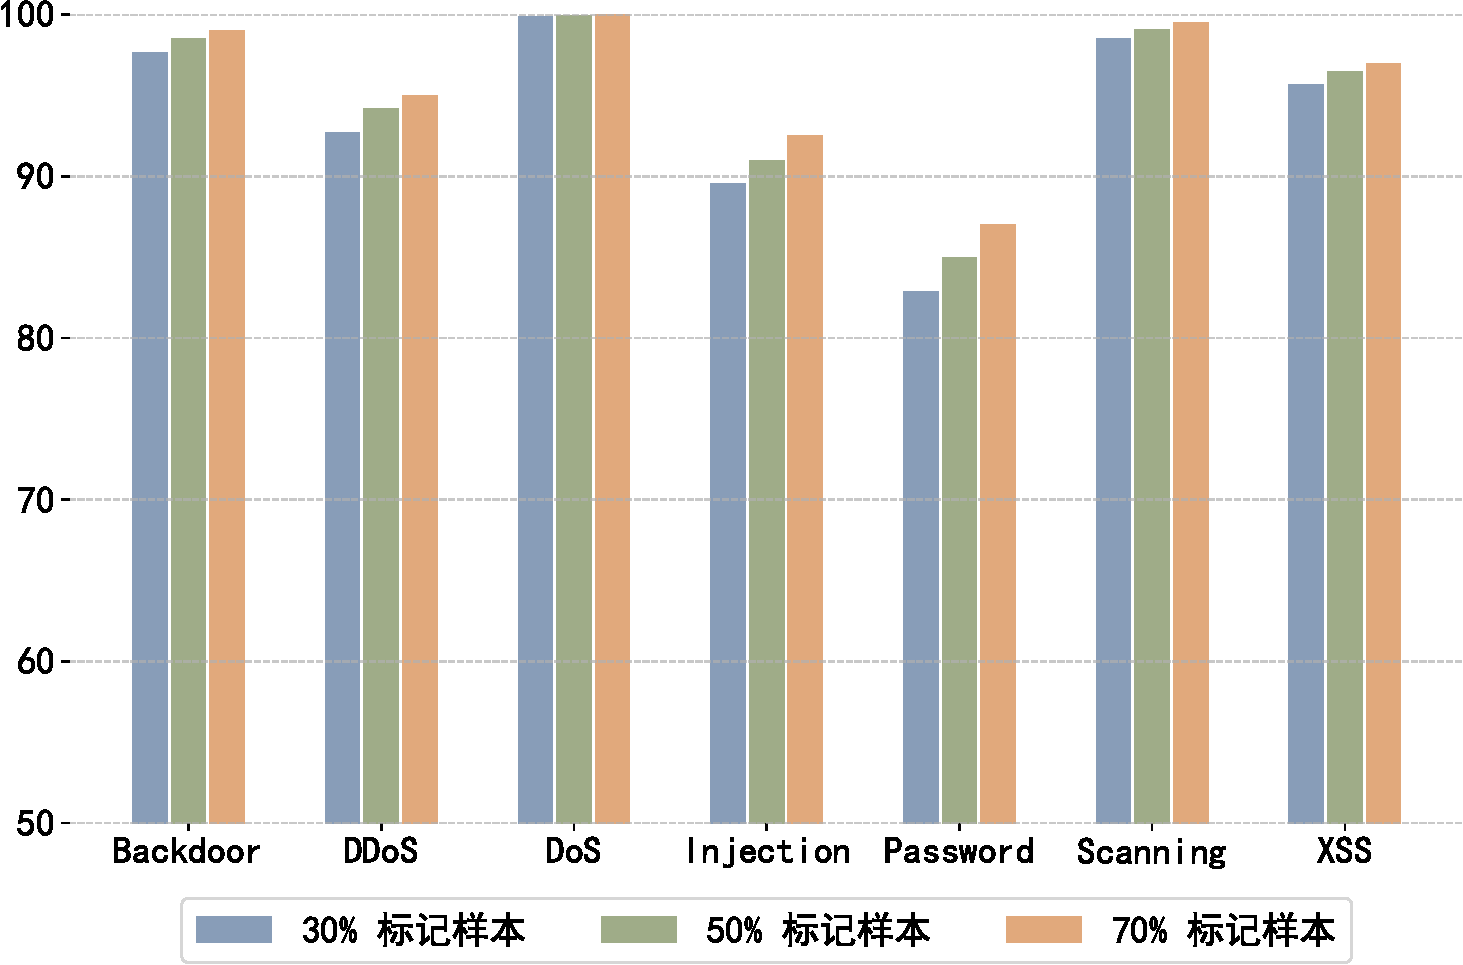
\includegraphics[width=1\linewidth]{./pic/chart3.pdf}
    \caption{在NF-ToN-IoT-V2数据集上进行半监督学习时在不同标签比例下实现的准确率}
    \label{AccOnNF-ToN-IoT-V2}
\end{figure}
为了进一步探索模型的表现能力,在 NF-CSE-CIC-IDS2018-V2 和 NF-ToN-IoT-V2 数据集上进行了半监督训练,使用了30\%、50\%和70\%的标记样本。通过观察图\ref{AccOnNF-ToN-IoT-V2}和图\ref{AccOnNF-CSE-CIC-IDS2018-V2}中的结果,可以看出对于这两个数据集中的每个类别,使用30\%标记样本的效果与使用70\%标记样本的效果并没有显著差距。

具体来说,在 NF-CSE-CIC-IDS2018-V2 数据集上,使用30\%标记样本的模型准确率与使用70\%标记样本准确率基本持平甚至略高。同样地,在 NF-ToN-IoT-V2 数据集上,使用30\%标记样本时,XSS攻击检测模型准确率为 95.7\%,而使用70\%标记样本时,准确率为 97.0\%,仅下降了 1.3\%。


这些结果表明,即使只标记了30\%的样本,模型仍然表现出非常强的表达能力和区分能力,能够有效地识别不同类型的网络攻击。与传统的全监督训练方法相比,这种半监督方法不仅减少了标注成本,同时也证明了该模型在处理不完全标注的数据时仍然能够保持较高的准确性和稳定性。


\begin{figure}[h!]
    \centering
    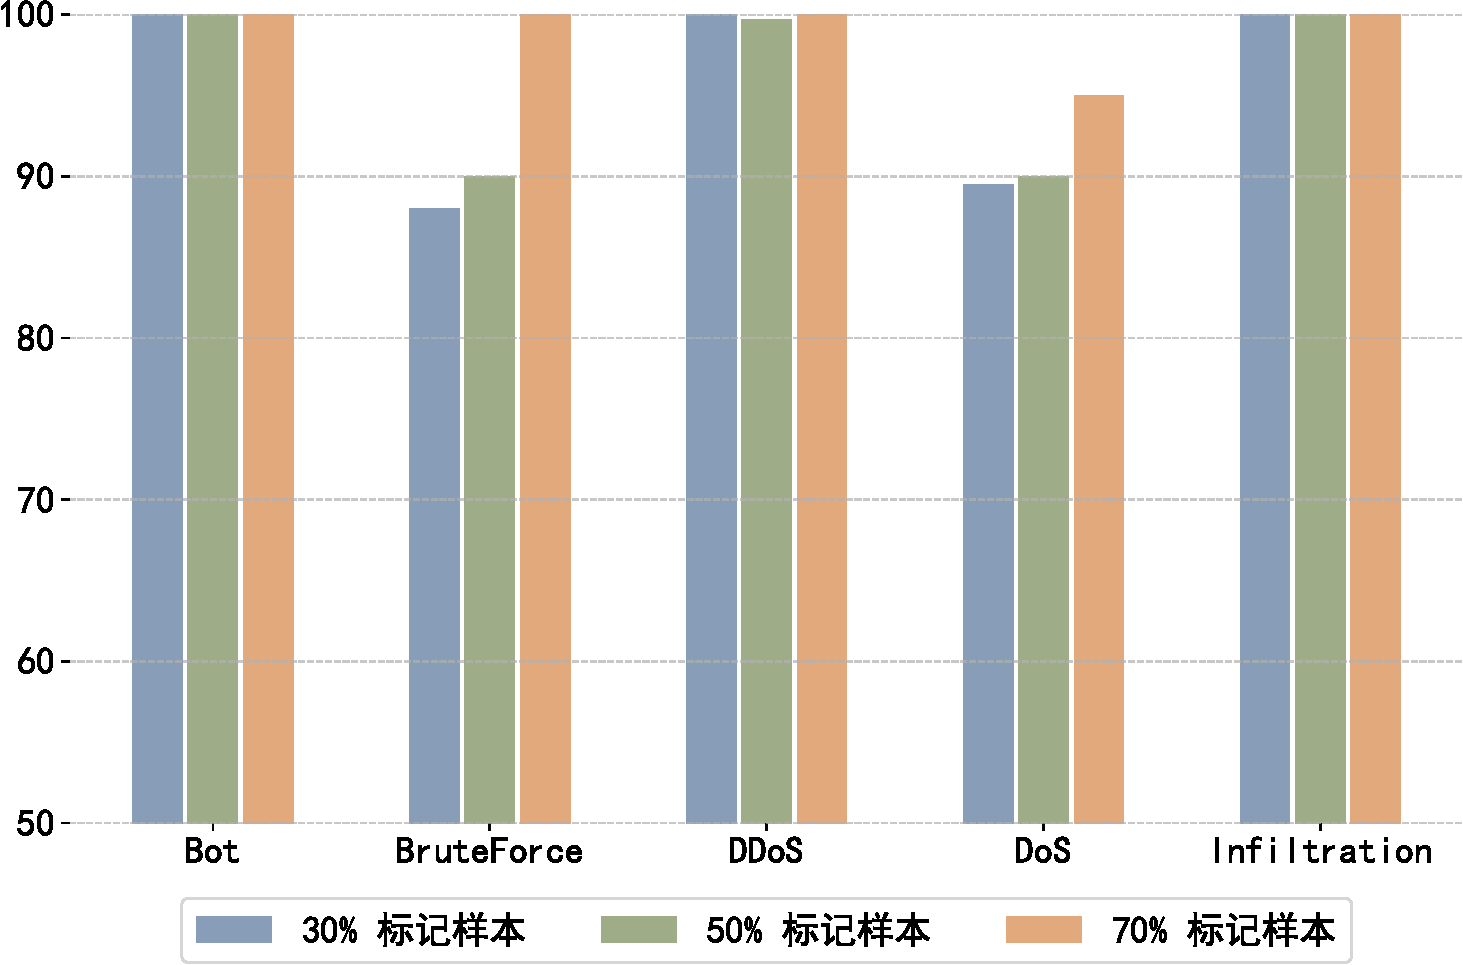
\includegraphics[width=1\linewidth]{./pic/chart2.pdf}
    \caption{在 NF-CSE-CIC-IDS2018-V2 数据集上进行半监督学习时在不同标签比例下实现的准确率}
    \label{AccOnNF-CSE-CIC-IDS2018-V2}
\end{figure}



\begin{table}[h!]
\centering
\caption{消融实验结果}
\begin{tabular}{c ||c c c}
\hline\hline
\textbf{Model} & \textbf{Dataset} & \textbf{ACC} & \textbf{F1} \\ \hline
LG-MTD & NF-BoT-IoT-V2 & 99.78\% & 0.9989 \\ \hline
LG-MTD without time-evolving features & NF-BoT-IoT-V2 & 91.74\% & 0.9233 \\ \hline
LG-MTD & NF-ToN-IoT-V2 & 98.69\% & 0.9887  \\ \hline
LG-MTD without time-evolving features & NF-ToN-IoT-V2 & 89.43\% & 0.8945 \\ \hline
LG-MTD & NF-BoT-IoT-V2 & 99.78\% & 0.9989 \\ \hline
LG-MTD without lineGraph & NF-BoT-IoT-V2 & 98.16\% & 0.9100 \\ \hline
LG-MTD & NF-ToN-IoT-V2 & 98.69\% & 0.9887 \\ \hline
LG-MTD without lineGraph & NF-ToN-IoT-V2 & 97.16\% & 0.9300 \\ \hline
GraphSAGE+line graph & NF-BoT-IoT & 85.30\% & 0.8500 \\ \hline
E-GraphSAGE & NF-BoT-IoT & 80.56\% & 0.8250 \\ \hline
GraphSAGE+line graph & NF-ToN-IoT & 75.10\% & 0.7800 \\ \hline
E-GraphSAGE & NF-ToN-IoT & 72.22\% & 0.6900 \\ \hline\hline
\end{tabular}
\label{resultofablation}
\end{table}
3.消融实验

第一项消融研究检查了时间演变相关性对最终入侵检测性能的影响。在这个实验中,去除了融合时空特征的 GCNII GRU 层,以切断时间演变信息在不同图快照之间的传播。也就是说,只利用 GCNII 层从多个图中学习网络流量统计和网络拓扑信息,并观察在没有时间演变特征参与的情况下实现的检测性能。如表\ref{resultofablation} 所示,当仅使用网络的拓扑信息和统计特征时,检测的 ACC 和 F1 分数值会下降。基于这些发现,表明考虑网络流量的“演变信息”确实有助于理解和描述网络行为。

为了以有效和直观的方式了解折线图的作用及其广泛的适用性, 采用当前模型和E-GraphSAGE 模型的折线图版本进行了验证实验。如前所述,E-GraphSAGE 通过 GraphSAGE 卷积操作在图边缘部署消息传递机制。因此,通过采用原始版本(GraphSAGE)与线图结构相结合进行了对比实验。表 \ref{resultofablation}中所示的比较实验结果表明,具有线形图结构的 GraphSAGE 比 E-GraphSAGE 实现了更高的检出率和 F1 分数值。这些结果表明,线图结构可以增强图卷积运算,而且这种效果不仅限于特定的图卷积层。

\section{本章小结}
本章提出了一种基于线图的恶意流量检测方法(LG-MTD),通过利用自适应注意力机制和线图结构提升图神经网络处理复杂图数据的能力。
首先,结合第三章的数据增强技术,构建了线图结构,使得模型能够更有效地捕捉边的特征。应用自适应多头注意力机制,
在图神经网络中动态调整节点间的注意力权重,实现更加精确的信息传递与特征聚合。引入MAD指标评估不同层次上节点特征的变化,
分析模型在处理不同类型节点和边时的鲁棒性。结合半监督学习方法,在有限的标注数据基础上,利用未标注数据进行训练,提升模型性能。
通过余弦相似度划分数据集,并结合MAD指标优化数据分布,确保训练集和测试集的有效性。此方法能有效提升图神经网络在半监督学习场景下的学习效果。
通过该方法,能够克服现有图神经网络的局限性,特别是在节点间关系动态变化和远程节点特征传递方面。通过在多个数据集上进行广泛严谨实验,
验证了所提出方法的有效性和鲁棒性。实验结果表明,LG-MTD在准确率、召回率、精确度和F1-Score等指标上均优于现有方法,
尤其在低误报率方面表现突出。通过对比分析,进一步验证了线图结构和自适应注意力机制在恶意流量检测中的重要性和有效性。

% \chapter{实验结果分析}
% \section{实验数据及环境}
% \subsection{实验环境}
% 本章所提的LDNFDDPM和LG-MTD方法在配备3.50GHz的12核Intel(R)\\Core(TM)i9-10920X
%  CPU、256 GB 内存和Linux 内核v.5.11.0 的 Ubuntu 20.04 LTS 操作系统上进行评
% 估。选用PyTorchv1.7.0 与 Jupyter notebook 一起实现相关实验,具体实验设置如
% 表\ref{tbl:hardware_config}所示。
% \begin{table}[h!]
%     \centering
%     \caption{硬件配置}
%     % \resizebox{\textwidth}{!}{
%     \begin{tabular}{c||c} \hline\hline
%         \textbf{名称} & \textbf{配置} \\ \hline
%         CPU & i9-10920X \\ \hline
%         GPU & 技嘉RTX3080 \\ \hline
%         内存 & 镁光256GB 3200HZ 8 \\ \hline
%         硬盘 & 三星2TB 2 \\ \hline\hline
%     \end{tabular}
%     \label{tbl:hardware_config}
%     % }
% \end{table}

% \subsection{实验数据}

% \begin{table}[h!]
%     \centering
%     \caption{NF-BoT-IoT-V2 数据集主要属性}
%     \begin{tabular}{c||c} \hline\hline
%         \textbf{属性} & \textbf{描述} \\ \hline
%         流量总数 & 37,763,497 \\ \hline
%         良性流量比例 & 0.36\% \\ \hline
%         IP 地址数 & 293 \\ \hline
%         端口数量 & 65,536 \\ \hline
%         平均流持续时间 & $3.999 \times 10^6$ 毫秒 \\ \hline
%         平均输入字节数 & 546 \\ \hline
%         平均输出字节数 & 204 \\ \hline
%         TCP 标志数量 & 25 \\ \hline
%         支持协议类型 & ICMP、TCP、UDP \\ \hline
%         攻击类别 & Reconnaissance, DDoS, DoS, Theft  \\ \hline\hline
%     \end{tabular}
%     \label{tbl:nf_bot_iot_v2}
% \end{table}
% 本文采用NF-BoT-IoT-V2、NF-ToN-IoT-V2、NF-CSE-CIC-IDS2018-V2三个数据集\citing{sarhan2022towards},详细介绍如下:

% NF-BoT-IoT-V2 数据集是基于原始 BoT-IoT 数据集生成的,如表\ref{tbl:nf_bot_iot_v2}所示。BoT-IoT 数据集最初由澳大利亚国立计算机安全中心(ACCS)实验室创建。通过使用 nProbe 提取原始 PCAP 数据中的 43 个 NetFlow 特征,生成了该数据集。NF-BoT-IoT-V2 包含 37,763,497 条流量数据,其中良性流量比例仅为 0.36\%,其余均为攻击流量。该数据集覆盖了 293 个 IP 地址和 65,536 个端口,平均流持续时间为 $3.999 \times 10^6$ 毫秒。它的入站和出站流量字节数较低,分别为 546 和 204。其主要支持的协议类型包括 ICMP、TCP 和 UDP。NF-BoT-IoT-V2 的攻击类型涵盖了探测攻击、DDoS 攻击、DoS 攻击以及数据盗窃。作为物联网流量分析的一个重要数据集,NF-BoT-IoT-V2 在攻击类型和规模上具有显著的失衡性,适合用于异常检测和攻击分类的研究。

% \begin{table}[h!]
%     \centering
%     \caption{NF-ToN-IoT-V2 数据集主要属性}
%     \begin{tabular}{c||c} \hline\hline
%         \textbf{属性} & \textbf{描述} \\ \hline
%         流量总数 & 16,940,495 \\ \hline
%         良性流量比例 & 36.01\% \\ \hline
%         IP 地址数 & 29,245 \\ \hline
%         端口数量 & 65,536 \\ \hline
%         平均流持续时间 & $7.929 \times 10^5$ 毫秒 \\ \hline
%         平均输入字节数 & 726 \\ \hline
%         平均输出字节数 & 837 \\ \hline
%         TCP 标志数量 & 34 \\ \hline
%         支持协议类型 & ICMP、TCP、UDP、IPv6-ICMP \\ \hline
%         攻击类别 &  DDoS, DoS, Backdoor,Injection,Password,Scanning,XSS \\ \hline\hline
%     \end{tabular}
%     \label{tbl:nf_ton_iot_v2}
% \end{table}
% NF-ToN-IoT-V2 数据集是 ToN-IoT 数据集的扩展版本,如表\ref{tbl:nf_ton_iot_v2}所示。NF-ToN-IoT-V2 数据集最初由澳大利亚国防部数据61实验室开发,旨在模拟真实物联网环境中的网络流量。该数据集包含 16,940,495 条网络流量,其中良性流量占 36.01\%。与其他物联网数据集相比,NF-ToN-IoT-V2 的流量数据覆盖范围较广,包括 29,245 个 IP 地址和 65,536 个端口,支持的协议类型包括 ICMP、TCP、UDP 和 IPv6-ICMP。平均流持续时间为 $7.929 \times 10^5$ 毫秒,入站和出站流量字节数分别为 726 和 837。NF-ToN-IoT-V2 中的攻击类型与 NF-BoT-IoT-V2 类似,主要包括探测攻击、DDoS 攻击、DoS 攻击和数据盗窃。该数据集具有更高的良性流量比例和丰富的流量特征,适合于物联网环境下的多协议分析和跨网络的异常检测研究。

% NF-CSE-CIC-IDS2018-V2 数据集基于原始 CICIDS2018 数据集生成,如表\ref{tbl:nf_cse_cic_ids2018_v2}所示。原始数据集由加拿大网络安全实验室(CIC)和通信安全研究中心(CSE)联合创建,旨在模拟现代企业网络中的攻击行为。该数据集包含 18,893,708 条网络流量,其中良性流量比例为 11.95\%。NF-CSE-CIC-IDS2018-V2 拥有 255,042 个独立 IP 地址和 65,492 个端口,协议类型覆盖范围广,包括 ICMP、TCP、UDP、IPv6-ICMP 和 GRE。平均流持续时间为 $5.746 \times 10^5$ 毫秒,入站和出站字节数分别为 1,812 和 6,913。该数据集的攻击类别多样化,包括暴力破解、僵尸网络、DoS 攻击、DDoS 攻击和渗透攻击等。NF-CSE-CIC-IDS2018-V2 数据集的特点在于其流量特征的多样性和复杂性,是研究企业网络安全威胁检测的重要资源,尤其适用于多种攻击类型的分类和流量分析任务。


% \begin{table}[h!]
%     \centering
%     \caption{NF-CSE-CIC-IDS2018-V2 数据集主要属性}
%     \begin{tabular}{c||c} \hline\hline
%         \textbf{属性} & \textbf{描述} \\ \hline
%         流量总数 & 18,893,708 \\ \hline
%         良性流量比例 & 11.95\% \\ \hline
%         IP 地址数 & 255,042 \\ \hline
%         端口数量 & 65,492 \\ \hline
%         平均流持续时间 & $5.746 \times 10^5$ 毫秒 \\ \hline
%         平均输入字节数 & 1,812 \\ \hline
%         平均输出字节数 & 6,913 \\ \hline
%         TCP 标志数量 & 50 \\ \hline\hline
%         支持协议类型 & ICMP、TCP、UDP、IPv6-ICMP、GRE \\ \hline
%         攻击类别 & BruteForce, Bot, DoS, DDoS, Infiltration \\ \hline\hline
%     \end{tabular}
%     \label{tbl:nf_cse_cic_ids2018_v2}
% \end{table}

% \section{实验设计}
% 本章实验工分为两个部分:数据增强方法实验、恶意流量检测方法实验。采用FID(Frechet Inception Distance)和IS( Inception Score )等指标来评估数据增强效果,采用准确率、召回率和F1-score等指标来评估检测效果。
% \subsection{评估指标}

% 混淆矩阵用于分类任务中,表示模型在不同类别上的预测结果。通过混淆矩阵可以计算多个关键指标,包括准确率、精确率、召回率和F1-Score等。二分类任务中的混淆矩阵结构如表\ref{ConfusionMatrix}所示:

% \begin{table}[h!]
%     \caption{混淆矩阵}
%     \begin{tabular}{c||c c}
%     \hline\hline
%     \textbf{} & \textbf{预测为正类} & \textbf{预测为负类} \\
%     \hline
%     真实为正类 & \text{TP (True Positive)} & \text{FN (False Negative)} \\\hline
    
%     真实为负类 & \text{FP (False Positive)} & \text{TN (True Negative)} \\
%     \hline\hline
%     \end{tabular}
%     \label{ConfusionMatrix}
% \end{table}

% 其中:
% TP:真正例,表示模型正确地将正类样本分类为正类。
% FP:假正例,表示模型错误地将负类样本分类为正类。
% TN:真负例,表示模型正确地将负类样本分类为负类。
% FN:假负例,表示模型错误地将正类样本分类为负类。


% (1)准确率 (Accuracy)

% 准确率指模型正确分类的样本数与总样本数之比,计算公式如\ref{Acc}所示:
% \begin{equation}
% \text{Accuracy} = \frac{TP + TN}{TP + TN + FP + FN}
% \label{Acc}
% \end{equation}

% (2)精确率 (Precision)

% 精确率是指在所有被模型预测为正类的样本中,实际上确实是正类的比例,计算公式如\ref{Pre}所示:
% \begin{equation}
% \text{Precision} = \frac{TP}{TP + FP}
% \label{Pre}
% \end{equation}

% (3)召回率 (Recall)

% 召回率指的是在所有实际为正类的样本中,模型正确预测为正类的比例,计算公式如\ref{Rec}所示:
% \begin{equation}
% \text{Recall} = \frac{TP}{TP + FN}
% \label{Rec}
% \end{equation}

% (4)F1-Score

% F1-Score是精确率和召回率的调和平均数,计算公式如\ref{F1}所示:
% \begin{equation}
% F1 = 2 \times \frac{\text{Precision} \times \text{Recall}}{\text{Precision} + \text{Recall}} = 2 \times \frac{TP}{2TP + FP + FN}
% \label{F1}
% \end{equation}

% (5)误报率 (False Positive Rate)

% 误报率衡量的是所有负类样本中,模型错误预测为正类的比例,计算公式如\ref{FPR}所示:
% \begin{equation}
% \text{False Positive Rate (FPR)} = \frac{FP}{FP + TN}
% \label{FPR}
% \end{equation}

% (6)FID

% FID是评估生成模型(如生成对抗网络的生成样本与真实样本之间的相似度)的指标。FID的原理是通过比较两个分布(真实数据和生成数据)在某一预训练网络(如Inception v3)上的特征表示来衡量它们之间的差距。

% \subsection{相关对比方法}
% 根据本文的研究方法和实验数据,针对数据增强和恶意流量检测部分,分别选择了近年来的优秀工作进行对比。为了评估 LDNFDDPM 在数据增强方面的效果,将其与其他现有数据增强方法进行了对比,如表\ref{dataAppend}所示:
% \begin{table}[h!]
% \centering
% \caption{数据增强方法对比}
% \resizebox{\textwidth}{!}{
% \begin{tabular}{>{\centering\arraybackslash}p{0.33\linewidth}||>{\centering\arraybackslash}p{0.33\linewidth}>{\centering\arraybackslash}p{0.34\linewidth}}  % 设置列宽
% \hline\hline
% \textbf{方法} & \textbf{描述} & \textbf{优缺点} \\
% \hline
% G-IDS \citing{shahriar2020g} & 利用基本的 GAN 生成流量数据,缓解数据不平衡问题。 & 生成的数据可能存在一定的偏差,训练效果有限。 \\
% \hline
% SIGMA \citing{msika2019sigma} & 使用随机森林对特征进行分割并使用 GAN 生成对抗样本。 & 生成的数据可能不能完全捕捉所有攻击流量特征。 \\
% \hline
% CWGAN-GP \citing{kang2022cwgan} & 基于 Wasserstein 距离的生成对抗网络,加入条件信息来改进数据生成。 & 生成的样本质量高,但模型训练相对复杂。 \\
% \hline
% SEMRes-DDPM \citing{zheng2024semres} & 基于去噪扩散概率模型,结合 SEMST-ResNet 提高数据生成质量。 & 需要较强的计算资源,模型复杂度较高。 \\
% \hline\hline
% \end{tabular}
% }
% \label{dataAppend}
% \end{table}




% G-IDS\citing{shahriar2020g}:G-IDS是一种基于GAN生成网络流量数据的技术,专门针对网络物理系统的数据不平衡问题。通过生成合成流量数据,G-IDS 可以增加少数类(如攻击流量)的样本量,从而提高入侵检测系统(IDS)的检测性能。虽然其生成的数据能够缓解数据不平衡的问题,但由于使用的是基本的 GAN,生成的数据可能存在一定的偏差和不足。

% SIGMA\citing{msika2019sigma}:SIGMA利用随机森林筛选关键特征,并结合GAN生成对抗样本,专为提升IDS在数据不平衡场景下的检测效能设计。尽管生成的数据能够增强模型的训练集,但由于 GAN 本身的局限性,生成的数据可能不能完全捕捉到所有攻击流量的特征。

% CWGAN-GP\citing{kang2022cwgan}:CWGAN-GP(条件Wasserstein生成对抗网络与梯度惩罚)是一种先进的深度生成对抗网络模型,专门用于处理不平衡数据问题。它通过引入条件信息来指导生成器生成特定类别的样本,从而在生成过程中更好地控制样本的类别分布。CWGAN-GP采用Wasserstein距离作为生成器和判别器之间的距离度量,相较于传统的GAN模型,能够更稳定地训练并生成高质量的样本。此外,该模型还引入了梯度惩罚机制,以替代传统的权重裁剪方法,进一步提高了模型的训练稳定性和生成样本的多样性。CWGAN-GP在生成合成数据以增强少数类样本方面表现出色,其广泛应用于图像生成、数据增强以及不平衡数据分类等领域,为解决数据不平衡问题提供了有效的解决方案。

% SEMRes-DDPM\citing{zheng2024semres}:SEMRes-DDPM是一种创新的过采样方法,专门针对不平衡表格数据的分类问题。它基于去噪扩散概率模型(DDPM),通过引入一种新颖的神经网络结构SEMST-ResNet来实现高效的去噪和数据合成。SEMST-ResNet结合了多头自注意力机制和软阈值处理,能够有效去除噪声并提取原始数据的特征,从而生成更接近真实数据分布的少数类样本。

% 为了评估LG-MTD在恶意流量方面的检测性能,选取了现有的几种物联网恶意流量检测方法进行比较,具体如表\ref{detectMethods}所示:



% \begin{table}[h!]
% \centering
% \caption{恶意流量检测方法对比}
% \resizebox{\textwidth}{!}{
% \begin{tabular}{c||>{\centering\arraybackslash}p{0.33\linewidth}>{\centering\arraybackslash}p{0.4\linewidth}}  % 设置列宽
% \hline\hline
% \textbf{方法} & \textbf{描述} & \textbf{优缺点} \\
% \hline
% E-GraphSAGE \citing{lo2022graphsage} & 基于图神经网络,捕捉边特征和拓扑信息。 &  适用于图结构数据,但对大数据处理复杂。 \\
% \hline
% Extra Trees \citing{sarhan2021netflow} &  基于决策树的集成学习方法,构建多个随机树分类。 &  高效处理大规模数据,但小样本效果较差。 \\
% \hline
% Random Forest (RF) \citing{rigatti2017random} &  通过多个决策树的投票结果进行分类,减少过拟合。 &  在大数据集上效果良好,但计算开销较大。 \\
% \hline
% DNN \citing{sarhan2022evaluating} &  深度前馈神经网络,自动学习复杂非线性关系。 &  计算资源消耗大,训练时间较长。 \\
% \hline
% TSVM \citing{abdel2021semi} &  半监督学习方法,利用少量标记数据提高性能。 &  标签数据稀缺时表现优秀,但处理大数据困难。 \\
% \hline\hline
% \end{tabular}
% }
% \label{detectMethods}
% \end{table}
% E-GraphSAGE\citing{lo2022graphsage}: E-GraphSAGE 是一种基于图神经网络的网络入侵检测方法。它通过同时捕捉流量数据中的边特征和拓扑信息来进行入侵检测。与传统的基于节点特征的 GNN 方法不同,E-GraphSAGE 强调了图中节点间的关系和数据流动方式,适用于具有复杂网络结构的入侵检测任务。通过从邻居节点聚合信息,E-GraphSAGE 能够有效捕捉到流量中的时序依赖和复杂的拓扑特征,在处理图结构数据时,表现出较强的性能。

% Extra Trees\citing{sarhan2021netflow}: Extra Trees 是一种基于决策树的集成学习方法,它通过构建多个极端随机树来进行分类。与随机森林类似,Extra Trees 使用了多个决策树的投票结果来进行决策,但它在训练过程中对特征的选择和切分点的选择引入了更多的随机性。这种方法在数据特征较多时,能够提高训练速度,并且具有较强的鲁棒性和较低的过拟合风险。Extra Trees 通常在处理大规模数据时表现出色,尤其是在数据存在噪声时。

% Random Forest (RF)\citing{rigatti2017random}: 随机森林是一种广泛使用的集成学习方法,通过建立多棵决策树来提高模型的准确性。每棵决策树独立训练于数据的随机子集和特征子集,因此它能够有效减少过拟合现象。随机森林的优点包括对异常值和噪声的鲁棒性强,能够自动评估特征的重要性,因此适用于处理具有高维度特征的数据。它在分类任务中,尤其是流量数据分类中表现良好,能够快速高效地处理大规模数据集。

% Deep Feedforward Neural Network (DNN)\citing{sarhan2022evaluating}: 深度前馈神经网络(DNN)是一种基础的神经网络模型,由多层全连接层组成,每一层通过激活函数将输入数据映射到新的空间。DNN 能够捕捉数据中的复杂非线性关系,尤其适用于处理高维度的结构化数据。在入侵检测任务中,DNN 能够从原始特征中自动学习出潜在的模式,从而提高分类性能。尽管 DNN 对计算资源的需求较高,但在数据量充足时,它能够通过深度学习方式处理更加复杂的特征关系。

% Transductive Support Vector Machine (TSVM)\citing{abdel2021semi}: TSVM 是一种半监督学习方法,旨在通过最大化标签数据和未标签数据之间的间隔来提高分类性能。它通过引入正则化项,约束分类超平面的选择,使得分类边界尽量远离未标记的数据,从而在数据稀缺的情况下实现更好的泛化能力。TSVM 在流量分类中的优势在于其能够利用少量的标记数据,同时结合大量的未标记数据进行训练,提高模型的鲁棒性和准确性,尤其在标签数据有限的情况下,TSVM 展现出了较强的优势。

% \section{数据增强方法实验}

% 数据增强方法的实验评估共分为两个部分:对比实验和消融实验。在对比实验中,评估LDNFDDPM及其它数据增强策略,通过计算每类攻击下10组随机生成样本的FID值,并重复10次取平均,以此均值作为标准,来衡量不同方法生成样本的质量,进一步验证生成数据的有效性,我们利用从原始数据训练的MLP模型评估生成样本的质量。在消融实验中,测试划分功能性特征于非功能性特征以及关注游离IP策略对于性能的影响。

% 1.对比实验

% 图\ref{FID}展示了各数据增强策略在不同数据集上的FID值对比,而表\ref{MethodsOnNF-BoT-IoT-V2}、表\ref{MethodsOnNF-CSE-CIC-IDS2018-V2}、\ref{MethodsOnNF-ToN-IoT-V2}和\ref{MethodsOnNF-ToN-IoT-V2_2}详细列出了这些增强算法生成样本在基于原始数据训练模型上的性能评估。

% \begin{figure}[h!]
%     \centering
%     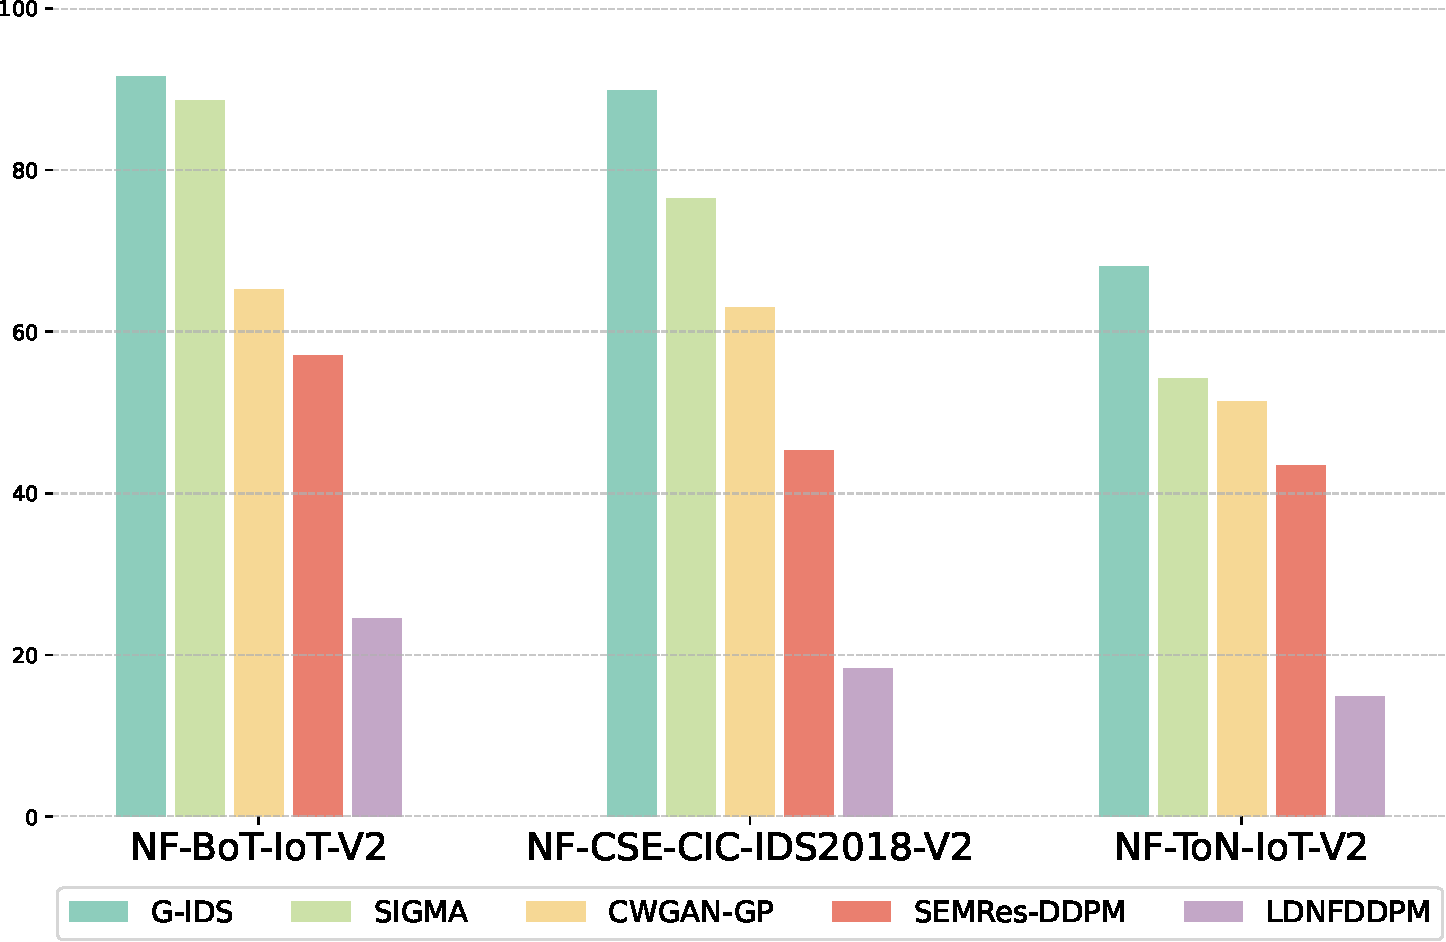
\includegraphics[width=1\linewidth]{./pic/chart1.pdf}
%     \caption{不同方法数据增强的效果表现}
%     \label{FID}
% \end{figure}
% (1)从整体来看,对于三个数据集上的FID表现来说,NF-BoT-IoT-V2略高于NF-CSE-CIC-IDS2018-V2,NF-CSE-CIC-IDS2018-V2略高于NF-ToN-IoT-V2。这是因为由于其攻击流量比例极高(99.64\%是攻击流量),且攻击类型较为简单,生成模型可能较容易生成攻击流量,但难以生成正常流量。虽然生成模型会聚焦于攻击流量的特征,但可能忽略了正常流量的多样性,这导致生成数据质量较低,FID 值较高。而NF-ToN-IoT-V2 良性流量比例相对较高(36.01\%),且该数据集包含多种协议(包括 IPv6-ICMP)。生成模型在生成攻击流量时的难度相对较大,但正常流量的特征较为明显,有助于生成模型较好地捕捉这些特征,因此 FID 值较低。对于NF-CSE-CIC-IDS2018-V2,该数据集复杂度最高,攻击类型多样,且协议种类丰富。生成模型在处理此类数据时需要学习到更复杂的特征,因此其 FID 处于两者之间。


% (2)观察图\ref{FID}可知,G-IDS和SIGMA等基于传统GAN生成的数据,FID值较高,且在表\ref{MethodsOnNF-BoT-IoT-V2}至\ref{MethodsOnNF-ToN-IoT-V2_2}的性能指标中,识别率(Rec)较低,暗示这些生成数据与真实数据存在显著差异。这归因于传统GAN在有限样本上的学习局限,导致模型难以全面捕获特征并良好适应小数据集。优化后的 GAN(CWGAN-GP)在表\ref{MethodsOnNF-BoT-IoT-V2}和表\ref{MethodsOnNF-CSE-CIC-IDS2018-V2}中生成数据的检测的表现要优于 G-IDS,但图\ref{FID}中 FID 值仍然较高。这表明,在训练 GAN时引入条件信息指导生成器生成特定类别的样本在一定程度上可以提高 GAN 性能。

% \begin{table}[h!]
% \centering
% \caption{NF-BoT-IoT-V2 数据集评估结果}
% \begin{tabular}{c||cccccccc}
% \hline\hline
% \multirow{2}{*}{Method} & \multicolumn{2}{c}{DDoS} & \multicolumn{2}{c}{DoS} & \multicolumn{2}{c}{Reconnaissance} & \multicolumn{2}{c}{Theft} \\
%                         & Pre         & Rec        & Pre        & Rec        & Pre              & Rec             & Pre         & Rec         \\ \hline
% \textbf{LDNFDDPM}       & \textbf{93.68} & \textbf{89.47} & \textbf{92.01} & \textbf{86.45} & \textbf{88.56}     & \textbf{83.56}    & \textbf{59.12} & \textbf{60.34} \\\hline
% G-IDS\citing{shahriar2020g}                   & 60.25       & 64.57      & 68.32      & 61.21      & 55.12            & 78.16           & 48.56       & 42.12       \\ \hline
% SIGMA\citing{msika2019sigma}                    & 72.14       & 67.54      & 80.34      & 74.13      & 67.10            & 71.24           & 52.12       & 45.79       \\ \hline
% CWGAN-GP\citing{kang2022cwgan}                 & 81.46       & 86.42      & 89.42      & 82.78      & 86.34            & 79.84           & 50.78       & 44.31       \\ \hline
% SEMRes-DDPM\citing{zheng2024semres}                & 90.24       & 81.91      & 81.42      & 85.54      & 88.02            & 72.63           & 53.45       & 47.46       \\ 
% \hline\hline
% \end{tabular}
% \label{MethodsOnNF-BoT-IoT-V2}
% \end{table}
% \begin{table}[h!]
% \centering
% \caption{NF-CSE-CIC-IDS2018-V2 数据集评估结果}
% \resizebox{\textwidth}{!}{
% \begin{tabular}{c||cccccccccc}
% \hline\hline
% \multirow{2}{*}{Method} & \multicolumn{2}{c}{DDos} & \multicolumn{2}{c}{Dos} & \multicolumn{2}{c}{Bot} & \multicolumn{2}{c}{BruteForce} & \multicolumn{2}{c}{Infiltration}                  \\
%                         & Pre         & Rec        & Pre      & Rec          & Pre        & Rec        & Pre            & Rec           & \multicolumn{1}{c}{Pre} & \multicolumn{1}{c}{Rec} \\ \hline
% \textbf{LDNFDDPM}       & \textbf{98.48} & \textbf{96.32} & \textbf{97.10} & \textbf{94.17} & \textbf{99.56} & \textbf{98.96} & \textbf{99.32} & \textbf{98.31} & \textbf{96.02} & \textbf{91.95} \\\hline
% G-IDS\citing{shahriar2020g}                   & 66.42       & 62.18      & 54.72      & 59.01      & 68.05       & 55.14      & 77.98         & 64.98        & 63.56       & 66.23       \\ \hline
% SIGMA\citing{msika2019sigma}                   & 77.58       & 74.63      & 76.12      & 62.28      & 68.78       & 67.11      & 78.64         & 66.67        & 74.98       & 79.48       \\ \hline
% CWGAN-GP\citing{kang2022cwgan}                  & 77.10       & 73.67      & 75.68      & 71.42      & 78.42       & 76.32      & 78.28         & 75.84        & 64.45       & 68.56       \\ \hline
% SEMRes-DDPM\citing{zheng2024semres}                & 88.05       & 93.56      & 91.78      & 93.54      & 92.14       & 88.24      & 89.02         & 90.59        & 94.68       & 91.24       \\ 
% \hline\hline  

% \end{tabular}
% \label{MethodsOnNF-CSE-CIC-IDS2018-V2}
% }
% \end{table}
% % Please add the following required packages to your document preamble:
% % \usepackage{multirow}
% \begin{table}[h!]
% \centering
% \caption{NF-ToN-IoT-V2 数据集评估结果}
% \begin{tabular}{c||ccccccccc}
% \hline\hline
% \multirow{2}{*}{Method} & \multicolumn{2}{c}{DDoS} & \multicolumn{2}{c}{DoS} & \multicolumn{2}{c}{Backdoor} & \multicolumn{2}{c}{XSS} \\
%                         & Pre         & Rec        & Pre        & Rec        & Pre           & Rec          & Pre        & Rec        \\ \hline
% \textbf{LDNFDDPM}       & \textbf{94.68} & \textbf{91.47} & \textbf{92.12} & \textbf{88.42} & \textbf{98.56} & \textbf{97.28} & \textbf{86.34} & \textbf{81.23} \\\hline
% G-IDS\citing{shahriar2020g}                    & 60.15       & 67.54      & 57.32      & 32.34      & 65.86         & 64.23        & 70.23      & 45.12      \\ \hline
% SIGMA\citing{msika2019sigma}                   & 72.30       & 79.73      & 70.42      & 66.37      & 67.08         & 65.54        & 63.47      & 78.21      \\ \hline
% CWGAN-GP\citing{kang2022cwgan}                  & 81.42       & 88.56      & 89.18      & 84.52      & 76.32         & 84.72        & 82.15      & 76.98      \\ \hline
% SEMRes-DDPM\citing{zheng2024semres}                & 93.75       & 90.59      & 91.56      & 87.74      & 98.12         & 96.75        & 84.96      & 79.87      \\ 
% \hline\hline
% \end{tabular}
% \label{MethodsOnNF-ToN-IoT-V2}
% \end{table}
% (3)与其他类型的数据增强方法相比,基于DDPM的方法(SEMRes-DDPM、LDNFDDPM)的FID值明显更低。这是因为DDPM通过逐步去噪的过程生成数据,避免了GAN中的模式崩溃和训练不稳定的问题,同时能够生成更加多样且高质量的样本。DDPM不依赖于生成器和判别器的对抗博弈,而是通过最大化数据似然进行训练,这使得它在数据稀缺或复杂分布的情况下表现得更加鲁棒和可靠。相较于SEMRes-DDPM,LDNFDDPM展现出了更优的性能,体现在较低的FID值和在同类数据集上更高的识别率。这得益于它专注于生成非功能特征,同时通过加重游离IP的权重,增强了样本的真实感并简化了训练过程。







% % Please add the following required packages to your document preamble:
% % \usepackage{multirow}
% \begin{table}[h!]
% \centering
% \caption{NF-ToN-IoT-V2 数据集评估结果(续表)}
% \begin{tabular}{c||cccccc}
% \hline\hline
% \multirow{2}{*}{Method} & \multicolumn{2}{c}{Scanning} & \multicolumn{2}{c}{Injection} & \multicolumn{2}{c}{Password} \\
%                         & Pre        & Rec        & Pre        & Rec        & Pre           & Rec          \\ \hline
% \textbf{LDNFDDPM}       & \textbf{97.01} & \textbf{93.56} & \textbf{85.01} & \textbf{87.65} & \textbf{76.43} & \textbf{69.12} \\ \hline
% G-IDS\citing{shahriar2020g}                   & 63.45      & 59.17      & 69.56      & 53.52      & 60.58         & 63.12        \\ \hline
% SIGMA\citing{msika2019sigma}                   & 65.02      & 61.28      & 61.25      & 65.56      & 73.85         & 66.14        \\ \hline
% CWGAN-GP\citing{kang2022cwgan}                  & 74.12      & 79.94      & 80.34      & 84.35      & 72.42         & 64.71        \\ \hline
% SEMRes-DDPM\citing{zheng2024semres}                & 96.23      & 92.85      & 92.45      & 87.08      & 75.12         & 67.85        \\ 
% \hline\hline
% \end{tabular}
% \label{MethodsOnNF-ToN-IoT-V2_2}
% \end{table}

% 2.消融实验

% 此次实验的主要目的是测试划分功能/非功能特征以及关注游离IP行为对于数据增强效果的影响。本节基于此设计了两种变体:LDDDPM和NFDDPM。

% LDDDPM:不对特征进行功能性、非功能性划分,直接进行加噪去噪过程。

% NFDDPM:不对游离IP做额外处理。

% % Please add the following required packages to your document preamble:
% % \usepackage{multirow}
% \begin{table}[h!]
% \centering
% \caption{不同消融设置下的数据增强表现}
% \begin{tabular}{c||ccc}
% \hline\hline
% \multirow{2}{*}{Method} & \multicolumn{3}{c}{FID}                               \\
%                         & NF-BoT-IoT-V2 & NF-CSE-CIC-IDS2018-V2 & NF-ToN-IoT-V2 \\ \hline
% \textbf{LDNFDDPM}                & \textbf{24.50}         & \textbf{18.30}                 & \textbf{14.90}        \\\hline
% LDDDPM                  & 47.15         & 41.54                 & 37.32         \\ \hline
% NFDDPM                  & 46.28         & 42.56                 & 34.17         \\
% \hline\hline
% \end{tabular}
% \label{Data_augmentation_based_on_ablation}
% \end{table}

% 各变体在不同数据集上的实验结果如表\ref{Data_augmentation_based_on_ablation}所示,可以看出,LDNFDDPM的FID值要低于LDDDPM,这表明,LDNFDDPM通过保存数据功能性特征,有助于生成模拟数据。同样,LDNFDDPM的FID值要低于NFDDPM,这表明,关注游离IP,对生成数据的真实性有一定提升。此外,在数据集NF-ToN-IoT-V2上NFDDPM的FID值要小于LDDDPM,这是因为NF-ToN-IoT-V2数据集的游离IP偏多,这也恰恰说明针对游离IP进行权重提升能够提高生成数据的真实性。


% 为了深入探讨滑动窗口和重叠率设计对入侵检测性能的影响,本实验去除了滑动窗口机制中的重叠率,即完全使用不重叠的窗口进行图快照切割,并观察在没有滑动窗口重叠的情况下,模型的检测性能变化。
% 具体而言,网络流量数据被按时间戳切割成多个图快照,每个快照仅代表某个特定的时间段,且相邻的快照之间没有重叠部分。在此框架下,模型仅依赖于这些不重叠的图快照中的网络拓扑信息进行训练。

% 如表\ref{table:ablation_window_overlap}所示,当没有滑动窗口重叠(重叠率为0)时,模型的准确率(ACC)和F1分数显著下降。这表明,当没有滑动窗口机制的支持时,网络流量的动态演变信息未能得到有效捕捉,导致模型在处理长时间序列时表现不佳。
% 特别是,在较长的时间序列中,网络流量的突发性变化无法通过单一的图快照反映出来,从而影响了检测性能。

% 进一步地,在使用不同重叠率(0、0.3、0.5、0.9)的滑动窗口机制进行实验时,结果显示随着重叠率的增加,模型的性能逐步提升。具体来说,当重叠率为0.3、0.5、0.9时,模型的ACC分别为0.9264、0.9311、0.9466,F1分数也随之增加。
% 此实验结果表明,滑动窗口的重叠率有助于捕捉到更丰富的时序信息,提升了模型在长时间序列中的稳定性和检测精度。

% 此外,随着滑动窗口重叠率的增加,模型的准确率方差从0.017下降至0.014,这进一步证明了滑动窗口机制能够提高模型在长时间序列场景中的数值稳定性。总体而言,滑动窗口和重叠率设计在捕捉网络流量的长期依赖性和时序变化方面发挥了重要作用,
% 尤其在面对网络攻击的长期演化过程中,能够显著提升检测性能。
% \begin{table}[h!]
%     \centering
%     \caption{滑动窗口与重叠率设计的消融实验结果}
%     \label{table:ablation_window_overlap}
%     \begin{tabular}{c||ccc}
%     \hline
%     \textbf{重叠率} & \textbf{准确率 (ACC)} & \textbf{F1分数} & \textbf{准确率方差} \\ \hline
%     0.0             & 0.9203               & 0.9102          & 0.017             \\ \hline
%     0.3             & 0.9264               & 0.9155          & 0.016             \\ \hline
%     0.5             & 0.9311               & 0.9198          & 0.015             \\ \hline
%     0.9             & 0.9466               & 0.9273          & 0.014             \\ \hline
%     \end{tabular}
% \end{table}
    

% \section{恶意流量检测方法实验}
% 在本实验中,将针对模型的性能和实际应用进行三个系列的实验分析:分类效果实验、不同监督比例实验和消融实验。
% 分类效果实验,以评估模型在不同数据集上的分类精度、召回率、精确度和 F1-Score等关键指标。不同监督比率的样本对模型性能的影响,通过调整标签数据的比例,观察模型在标注数据稀缺情况下的表现。消融研究通过逐个移除模型组件,
% 来量化每个部分对整体性能的影响。通过这些实验,旨在全面评估模型在不同条件下的鲁棒性和有效性。

% 在本实验中,使用了一些关键的超参数来调整模型的训练过程。表\ref{Hyperparameters}列出了模型的默认超参数值及其相应的描述:

% \begin{table}[h!]
% \centering
% \caption{模型的默认超参数值}
% \begin{tabular}{ c || c c }
% \hline\hline
% \textbf{超参数} & \textbf{描述} & \textbf{默认值} \\
% \hline
% \textbf{Learning rate} & 每次迭代时朝着损失函数最小值前进的步长 & 0.001 \\
% \hline
% \textbf{Weight decay} & 损失函数的 L2 惩罚项 & 0.001 \\
% \hline
% \textbf{Sequence length} & 每个批次中的网络快照数量 & 100 \\
% \hline
% \textbf{Sliding window overlap} & 连续快照之间的重叠部分 & 50\% \\
% \hline
% \textbf{Early stop patience} & 在最后一次验证损失改进后等待的轮数 & 20 \\
% \hline\hline
% \end{tabular}
% \label{Hyperparameters}
% \end{table}
% 1.分类效果分析

% 在三个数据集的分析中,LG-MTD 表现出了显著的优势,如表\ref{tab:nf_bot_iot_v2}、\ref{tab:nf_ton_iot_v2}和\ref{tab:nf_cse_cic_ids2018_v2}所示。

% 在 NF-BoT-IoT-V2 数据集上,LG-MTD 的准确率为 99.78\%,远高于其他对比方法。尽管 RandomForest 和 DNN 的准确率分别为 100\% 和 99.54\%,它们的误报率(FAR)较高,尤其是 DNN 方法的误报率为 0.20\%,而 LG-MTD 的误报率为 0.01\%,显示出其更强的鲁棒性。在召回率方面,LG-MTD 的值为 0.9998,几乎达到了完美,且精确度(0.9979)也优于其他方法。总体来看,LG-MTD 在综合性能(准确率、召回率、精确度和 F1-Score)上都表现得非常优秀,尤其是在低误报率方面,显示了更高的检测可靠性。

% 在 NF-ToN-IoT-V2 数据集上,LG-MTD 的准确率为 98.69\%,略低于 E-GraphSAGE(99.69\%)和 ExtraTrees(99.66\%)。尽管如此,LG-MTD 在召回率(0.9794)和精确度(0.9982)方面仍保持了较高水平,显示出其在减少假阳性(精确度)和提高检测率(召回率)方面的平衡能力。与 RandomForest 和 DNN 相比,LG-MTD 在误报率(FAR)上表现更为优秀,尤其在减少假阳性方面表现突出。

% 在 NF-CSE-CIC-IDS2018-V2 数据集上,LG-MTD 的表现更为显著,其准确率为 99.80\%,大幅领先于其他方法。ExtraTrees 的准确率为 95.33\%,而 TSVM 的准确率仅为 91.22\%。在召回率方面,LG-MTD 为 0.9986,几乎完美,远超 ExtraTrees 和 TSVM。在精确度上,LG-MTD 的值为 0.9988,接近完美,而 ExtraTrees 的精确度较低,为 0.7420。F1-Score 指标也表明,LG-MTD(0.9987)明显优于 ExtraTrees(0.83)和 TSVM(0.9127)。最为关键的是,LG-MTD 的误报率为 0.13\%,在所有方法中最低,这在流量分类中非常重要,因为较低的误报率有助于减少系统负担。
% % 表格 1: NF-BoT-IoT-V2 数据集
% \begin{table}[h!]
% \centering
% \caption{ NF-BoT-IoT-V2 数据集方法对比}
% \label{tab:nf_bot_iot_v2}
% \begin{tabular}{c|| c c c c c c }
% \hline\hline
% \textbf{Method} & \textbf{Accuracy} & \textbf{Recall} & \textbf{Precision} & \textbf{F1-Score} & \textbf{FAR} \\ \hline
% \textbf{LG-MTD} & 99.78\% & 0.9998 & 0.9979 & 0.9989 & 0.01\% \\ \hline
% E-GraphSAGE\citing{lo2022graphsage} & 93.57\% & 0.9343 & 1.0 & 0.97 & 0.38\% \\ \hline
% ExtraTrees\citing{sarhan2021netflow} & 93.82\% & 1.0 & 0.9417 & 0.97 & 1.13\% \\ \hline
% RandomForest\citing{sarhan2022evaluating} & 100.0\% & 1.0 & 1.0 & 1.0 & 0.25\% \\ \hline
% DNN\citing{sarhan2022evaluating} & 99.54\% & 0.9954 & 1.0 & 1.0 & 0.20\% \\ \hline
% TSVM\citing{abdel2021semi} & 92.0\% & 0.91 & 0.92 & 0.915 & 7.5\% \\ \hline\hline
% \end{tabular}
% \end{table}

% % 表格 2: NF-ToN-IoT-V2 数据集
% \begin{table}[h!]
% \centering
% \caption{ NF-ToN-IoT-V2 数据集方法对比}
% \label{tab:nf_ton_iot_v2}
% \begin{tabular}{ c|| c c c c c c }
% \hline\hline
% \textbf{Method} & \textbf{Accuracy} & \textbf{Recall} & \textbf{Precision} & \textbf{F1-Score} & \textbf{FAR} \\ \hline
% \textbf{LG-MTD} & 98.69\% & 0.9794 & 0.9982 & 0.9887 & 2.05\% \\ \hline
% E-GraphSAGE\citing{lo2022graphsage} & 99.69\% & 0.9985 & 1.0 & 1.0 & 0.15\% \\ \hline
% ExtraTrees\citing{sarhan2021netflow} & 99.66\% & 0.9967 & 0.9995 & 1.0 & 0.37\% \\ \hline
% RandomForest\citing{sarhan2022evaluating} & 99.66\% & 0.9980 & 0.9991 & 1.0 & 0.58\% \\ \hline
% DNN\citing{sarhan2022evaluating} & 94.74\% & 0.9527 & 0.9674 & 0.96 & 6.08\% \\ \hline
% TSVM\citing{abdel2021semi} & 91.0\% & 0.89 & 0.91 & 0.90 & 7.5\% \\ \hline\hline
% \end{tabular}
% \end{table}
% 综合来看,LG-MTD 在所有三个数据集中的表现都非常优秀,尤其在准确率、召回率、精确度和 F1-Score 方面均表现突出。与 RandomForest 和 DNN 等方法相比,LG-MTD 在误报率方面更具优势。特别是在 NF-CSE-CIC-IDS2018-V2 数据集上,LG-MTD 展现了极强的稳定性和高效的流量分类能力,显示了其在处理复杂网络流量分类任务时的优势。

% % 表格 3: NF-CSE-CIC-IDS2018-V2 数据集
% \begin{table}[h!]
% \centering
% \caption{ NF-CSE-CIC-IDS2018-V2 数据集方法对比}
% \label{tab:nf_cse_cic_ids2018_v2}
% \begin{tabular}{ c|| c c c c c c }
% \hline\hline
% \textbf{Method} & \textbf{Accuracy} & \textbf{Recall} & \textbf{Precision} & \textbf{F1-Score} & \textbf{FAR} \\ \hline
% \textbf{LG-MTD} & 99.80\% & 0.9986 & 0.9988 & 0.9987 & 0.13\% \\ \hline
% E-GraphSAGE\citing{lo2022graphsage} & 93.0\% & 0.92 & 0.95 & 0.935 & 0.50\% \\ \hline
% ExtraTrees\citing{sarhan2021netflow} & 95.33\% & 0.9471 & 0.7420 & 0.83 & 4.59\% \\ \hline
% RandomForest\citing{sarhan2022evaluating} & 99.47\% & 0.9682 & 0.9921 & 0.98 & 0.17\% \\ \hline
% DNN\citing{sarhan2022evaluating} & 99.24\% & 0.9467 & 0.9944 & 0.97 & 0.14\% \\ \hline
% TSVM\citing{abdel2021semi} & 91.22\% & 0.9121 & 0.9133 & 0.9127 & 8.06\% \\ \hline\hline
% \end{tabular}
% \end{table}

% 另一方面,在三个不同的数据集上,所提出的 LG-MTD 方法显示出了较强的分类能力。特别是在 NF-CSE-CIC-IDS2018-V2 数据集上,几乎所有类别的准确率和 F1-Score 都达到了 100\%,并且加权平均的 F1-Score 高达 0.9996。这表明该模型在处理大多数类别时表现出了非常优越的分类性能,尤其是在 Bot、BruteForce、DDoS 和 Infiltration 类别上,均获得了完美的性能。

% 在 NF-ToN-IoT-V2 数据集上,LG-MTD 的表现较好,准确率分别为 92.68\%、99.89\% 和 98.51\%,且 F1-Score 也分别为 0.8919、0.9983 和 0.9778。尽管 Injection 和 Password 类别的表现相对较弱,准确率分别为 89.53\% 和 82.85\%,F1-Score 也偏低,但其他攻击类别的高准确率和 F1-Score 表明该模型在大多数类别上仍然表现良好。整体加权平均准确率为 93.37\%,F1-Score 为 0.9340,反映了该模型在大部分类别上的较为均衡的表现。

% 在 NF-CSE-CIC-IDS2018-V2 数据集上,Bot 和 Infiltration 类别的准确率和 F1-Score 达到 100\%,表明该模型在这两个类别上的分类表现极为优越。BruteForce 类别也表现出色,准确率为 100\%,F1-Score 为 1.0,表明该模型能够很好地捕捉这一攻击类别的特征。虽然 DoS 类别的准确率为 99.50\%,F1-Score 为 0.9924,但依然保持了很高的性能。整体加权平均准确率为 99.96\%,F1-Score 为 0.9996,显示出该模型在此数据集上的极高表现。

% 在 NF-BoT-IoT-V2 数据集上,DDoS 和 DoS 类别的表现较好,准确率分别为 99.05\% 和 95.95\%,F1-Score 为 0.9859 和 0.9399。Reconnaissance 类别的准确率和 F1-Score 稍微下降,准确率为 94.21\%,F1-Score 为 0.9146。Theft 类别的表现相对较弱,准确率仅为 59.08\%,F1-Score 为 0.4975,表明该类别在样本分布或特征提取方面可能存在一定问题。整体加权平均准确率为 95.72\%,F1-Score 为 0.9579,说明该模型在大多数类别上表现良好,但在少数类别上可能存在提升空间。

% \begin{table}[h!]
% \centering
% \caption{ NF-ToN-IoT-V2 数据集多分类结果}
% \begin{tabular}{c|| c c}
% \hline\hline
% \textbf{ClassName} & \textbf{ ACC} & \textbf{ F1-Score} \\
% \hline
% Backdoor\citing{gao2020backdoor} & 97.66\% & 0.9653 \\
% \hline
% DDoS\citing{mirkovic2004taxonomy} & 92.68\% & 0.8919 \\
% \hline
% DoS\citing{carl2006denial} & 99.89\% & 0.9983 \\
% \hline
% Injection\citing{alghawazi2022detection} & 89.53\% & 0.8459 \\
% \hline
% Password\citing{wang2021attacks} & 82.85\% & 0.7517 \\
% \hline
% Scanning\citing{lee2003detection} & 98.51\% & 0.9778 \\
% \hline
% XSS\citing{gupta2017cross} & 95.70\% & 0.9359 \\
% \hline
% Weighted Average & 93.37\% & 0.9340 \\
% \hline\hline
% \end{tabular}
% \label{Multi-classificationOnNF-ToN-IoT-V2}
% \end{table}
% \begin{table}[h!]
% \centering
% \caption{ NF-CSE-CIC-IDS2018-V2 数据集多分类结果}
% \begin{tabular}{c|| c c }
% \hline\hline
% \textbf{ClassName} & \textbf{ ACC} & \textbf{ F1-Score} \\
% \hline
% Bot\citing{zhang2011survey} & 100.00\% & 1.0 \\
% \hline
% BruteForce\citing{knudsen2011block} & 100.00\% & 1.0 \\
% \hline
% DDoS\citing{mirkovic2004taxonomy} & 100.00\% & 1.0 \\
% \hline
% DoS\citing{carl2006denial} & 99.50\% & 0.9924 \\
% \hline
% Infiltration\citing{陈可2023自动化渗透测试技术研究综述} & 100.00\% & 1.0 \\
% \hline
% Weighted Average & 99.96\% & 0.9996 \\
% \hline\hline
% \end{tabular}
% \label{Multi-classificationOnNF-CSE-CIC-IDS2018-V2}
% \end{table}
% \begin{table}[h!]
% \centering
% \caption{ NF-BoT-IoT-V2 数据集多分类结果}
% \begin{tabular}{c|| c c }
% \hline\hline
% \textbf{ClassName} & \textbf{ ACC} & \textbf{ F1-Score} \\
% \hline
% DDoS\citing{mirkovic2004taxonomy} & 99.05\% & 0.9859 \\
% \hline
% DoS\citing{carl2006denial} & 95.95\% & 0.9399 \\
% \hline
% Reconnaissance\citing{jafarian2015effective} & 94.21\% & 0.9146 \\
% \hline
% Theft\citing{leevy2021detecting} & 59.08\% & 0.4975 \\
% \hline
% Weighted Average & 95.72\% & 0.9579 \\
% \hline\hline
% \end{tabular}
% \label{Multi-classificationOnNF-BoT-IoT-V2}

% \end{table}
% LG-MTD 模型在大多数类别上具有非常强的分类能力,特别是在 NF-CSE-CIC-IDS2018-V2 和 NF-ToN-IoT-V2 数据集上,表现出色。对于 Bot、BruteForce、DDoS 等类别,LG-MTD 提供了几乎完美的分类结果,F1-Score 达到 1.0。从表\ref{Multi-classificationOnNF-BoT-IoT-V2}可以看到,对于Theft的表现略显不足,这是由于这Theft这类攻击类型仅占 NF-BoT-IoT-V2数据集的0.21\%,样本稀疏带来不稳定检测。加权平均准确率和 F1-Score 表现出模型在各个类别之间的平衡能力,尤其在 NF-CSE-CIC-IDS2018-V2 数据集上,模型的综合表现尤为突出,表明该模型在应对复杂场景下能够取得稳定的效果。










% 2.不同监督率的样本的影响

% \begin{figure}[h!]
%     \centering
%     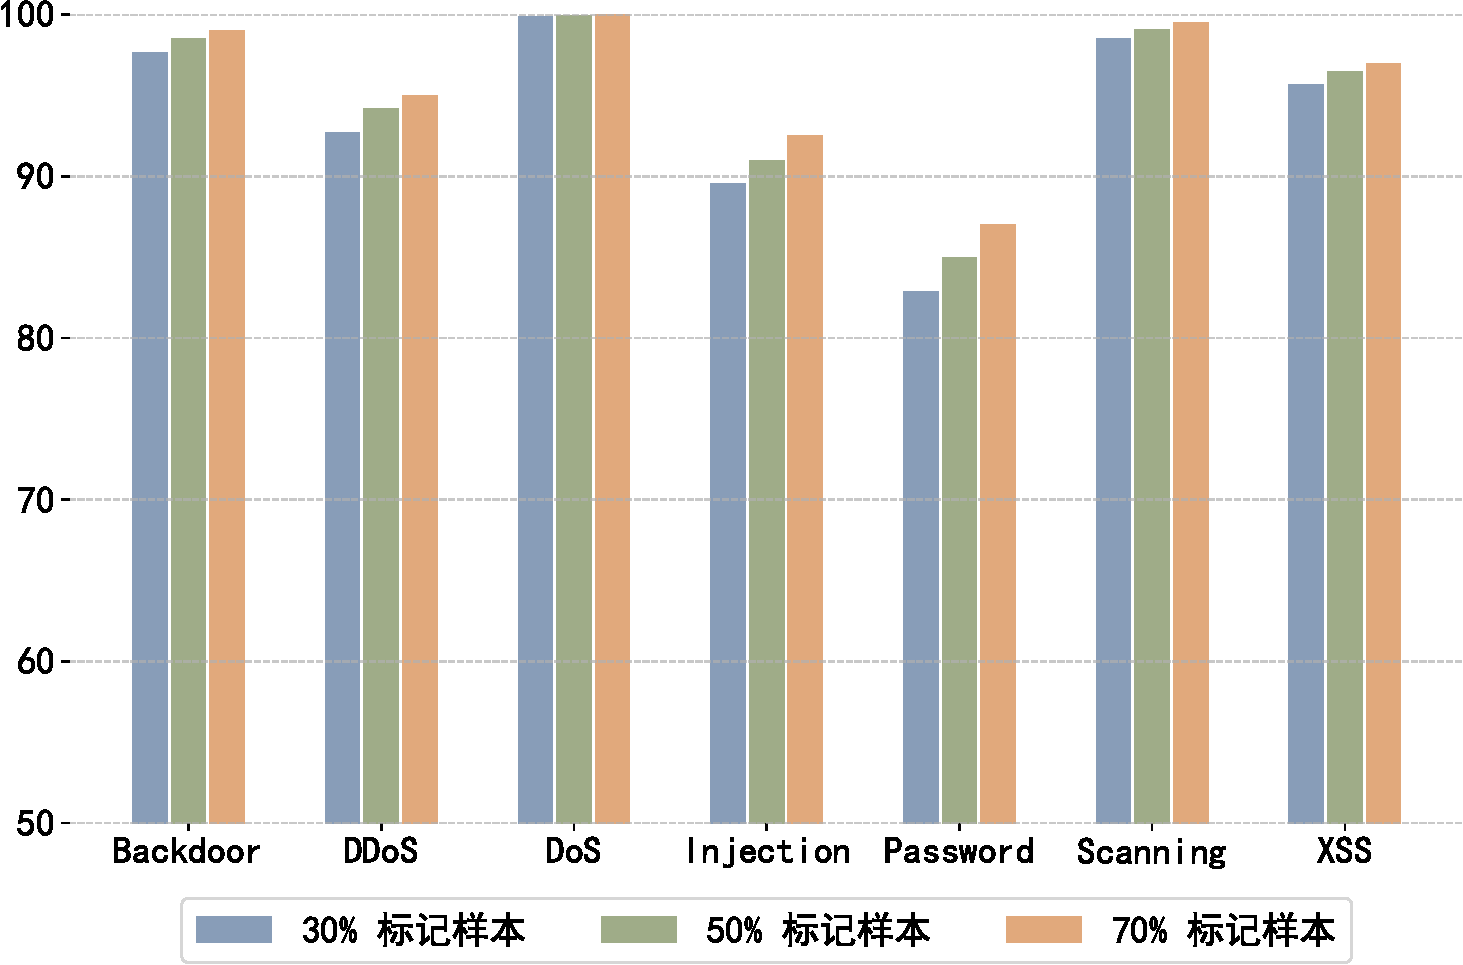
\includegraphics[width=1\linewidth]{./pic/chart3.pdf}
%     \caption{在NF-ToN-IoT-V2数据集上进行半监督学习时在不同标签比例下实现的准确率}
%     \label{AccOnNF-ToN-IoT-V2}
% \end{figure}
% 为了进一步探索模型的表现能力,在 NF-CSE-CIC-IDS2018-V2 和 NF-ToN-IoT-V2 数据集上进行了半监督训练,使用了30\%、50\%和70\%的标记样本。通过观察图\ref{AccOnNF-ToN-IoT-V2}和图\ref{AccOnNF-CSE-CIC-IDS2018-V2}中的结果,可以看出对于这两个数据集中的每个类别,使用30\%标记样本的效果与使用70\%标记样本的效果并没有显著差距。

% 具体来说,在 NF-CSE-CIC-IDS2018-V2 数据集上,使用30\%标记样本的模型准确率与使用70\%标记样本准确率基本持平甚至略高。同样地,在 NF-ToN-IoT-V2 数据集上,使用30\%标记样本时,XSS攻击检测模型准确率为 95.7\%,而使用70\%标记样本时,准确率为 97.0\%,仅下降了 1.3\%。


% 这些结果表明,即使只标记了30\%的样本,模型仍然表现出非常强的表达能力和区分能力,能够有效地识别不同类型的网络攻击。与传统的全监督训练方法相比,这种半监督方法不仅减少了标注成本,同时也证明了该模型在处理不完全标注的数据时仍然能够保持较高的准确性和稳定性。


% \begin{figure}[h!]
%     \centering
%     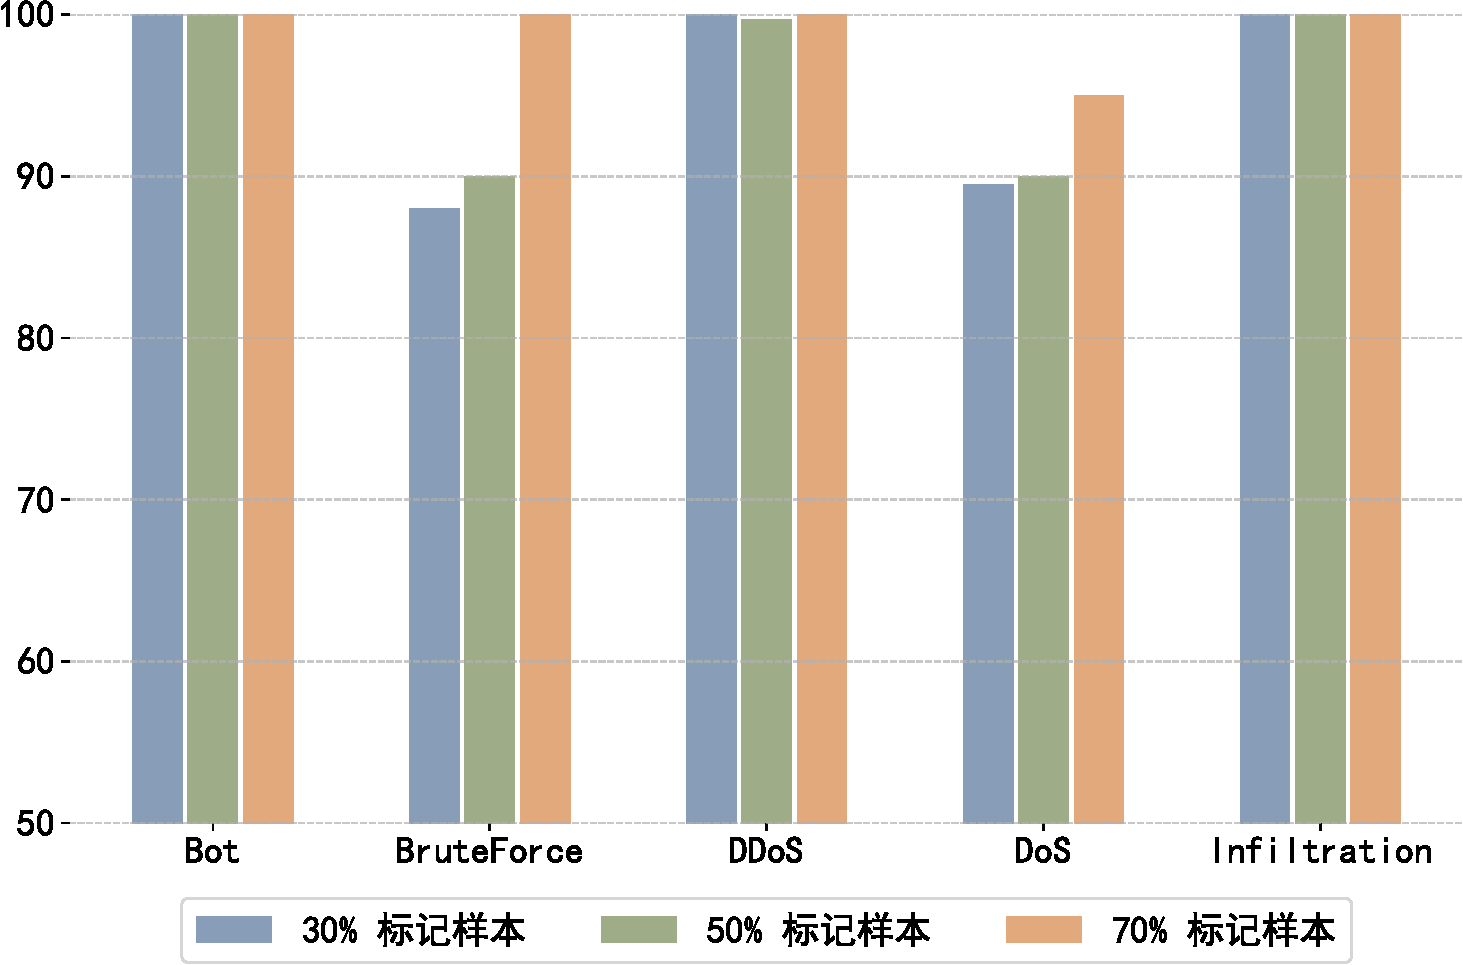
\includegraphics[width=1\linewidth]{./pic/chart2.pdf}
%     \caption{在 NF-CSE-CIC-IDS2018-V2 数据集上进行半监督学习时在不同标签比例下实现的准确率}
%     \label{AccOnNF-CSE-CIC-IDS2018-V2}
% \end{figure}



% \begin{table}[h!]
% \centering
% \caption{消融实验结果}
% \begin{tabular}{c ||c c c}
% \hline\hline
% \textbf{Model} & \textbf{Dataset} & \textbf{ACC} & \textbf{F1} \\ \hline
% LG-MTD & NF-BoT-IoT-V2 & 99.78\% & 0.9989 \\ \hline
% LG-MTD without time-evolving features & NF-BoT-IoT-V2 & 91.74\% & 0.9233 \\ \hline
% LG-MTD & NF-ToN-IoT-V2 & 98.69\% & 0.9887  \\ \hline
% LG-MTD without time-evolving features & NF-ToN-IoT-V2 & 89.43\% & 0.8945 \\ \hline
% LG-MTD & NF-BoT-IoT-V2 & 99.78\% & 0.9989 \\ \hline
% LG-MTD without lineGraph & NF-BoT-IoT-V2 & 98.16\% & 0.9100 \\ \hline
% LG-MTD & NF-ToN-IoT-V2 & 98.69\% & 0.9887 \\ \hline
% LG-MTD without lineGraph & NF-ToN-IoT-V2 & 97.16\% & 0.9300 \\ \hline
% GraphSAGE+line graph & NF-BoT-IoT & 85.30\% & 0.8500 \\ \hline
% E-GraphSAGE & NF-BoT-IoT & 80.56\% & 0.8250 \\ \hline
% GraphSAGE+line graph & NF-ToN-IoT & 75.10\% & 0.7800 \\ \hline
% E-GraphSAGE & NF-ToN-IoT & 72.22\% & 0.6900 \\ \hline\hline
% \end{tabular}
% \label{resultofablation}
% \end{table}
% 3.消融实验

% 第一项消融研究检查了时间演变相关性对最终入侵检测性能的影响。在这个实验中,去除了融合时空特征的 GCNII GRU 层,以切断时间演变信息在不同图快照之间的传播。也就是说,只利用 GCNII 层从多个图中学习网络流量统计和网络拓扑信息,并观察在没有时间演变特征参与的情况下实现的检测性能。如表\ref{resultofablation} 所示,当仅使用网络的拓扑信息和统计特征时,检测的 ACC 和 F1 分数值会下降。基于这些发现,表明考虑网络流量的“演变信息”确实有助于理解和描述网络行为。

% 为了以有效和直观的方式了解折线图的作用及其广泛的适用性, 采用当前模型和E-GraphSAGE 模型的折线图版本进行了验证实验。如前所述,E-GraphSAGE 通过 GraphSAGE 卷积操作在图边缘部署消息传递机制。因此,通过采用原始版本(GraphSAGE)与线图结构相结合进行了对比实验。表 \ref{resultofablation}中所示的比较实验结果表明,具有线形图结构的 GraphSAGE 比 E-GraphSAGE 实现了更高的检出率和 F1 分数值。这些结果表明,线图结构可以增强图卷积运算,而且这种效果不仅限于特定的图卷积层。






% \section{本章小结}


% 本章详细分析了实验环境、数据集和实验设计。在实验环境部分,介绍了硬件配置和操作系统,确保实验的重复性和结果的可靠性。数据集部分则描述了NF-BoT-IoT-V2、NF-ToN-IoT-V2和NF-CSE-CIC-IDS2018-V2三个数据集的特征,为后续对比分析提供基础。

% 在实验设计中,定义了准确率、精确率、召回率、F1-Score等评估指标,同时引入FID值来评估数据增强效果。通过与其他数据增强方法的对比,LDNFDDPM在生成样本质量和恶意流量检测性能上表现出较大优势。消融实验进一步验证了特征划分和游离IP策略对性能的影响。

% 实验结果表明,LDNFDDPM在数据增强和恶意流量检测中具有显著优势,证明其在物联网环境下的可行性和有效性。
\chapter{全文总结与展望}

\section{全文总结}

本文聚焦于物联网环境下的恶意流量检测问题,针对现有方法在数据不平衡、特征复杂性以及模型鲁棒性等方面的不足,提出了一种基于图神经网络和去噪扩散概率模型的创新检测方案。文章首先对恶意流量检测的背景、意义以及国内外研究现状进行了深入分析,明确了数据不平衡处理和恶意流量检测技术的研究重点。接着,详细介绍了相关理论及技术,包括恶意网络流量概念、去噪扩散模型、半监督学习、图神经网络、图卷积网络以及图注意力机制等,为后续方法设计奠定了坚实基础。

在方法设计方面,文章提出了两项关键技术:基于非功能性特征和低度 IP 的去噪扩散概率模型(LDNFDDPM)以及基于线图的恶意流量检测方法(LG-MTD)。LDNFDDPM 通过数据预处理、时序图构建和恶意流量生成等步骤,有效解决了流量数据中的不平衡问题,提升了模型对低度 IP 和稀有攻击类型的识别能力。该模型引入功能性与非功能性特征划分,保留关键特征的同时,利用 DDPM 生成非功能性特征,增强了数据的多样性和真实性。此外,通过构建时序图捕捉流量数据的时间依赖性,进一步提高了模型的鲁棒性。

基于线图的恶意流量检测方法则进一步优化了图神经网络的性能。该方法利用线图结构更有效地捕捉边的特征,通过多头注意力机制动态调整节点间的注意力权重,实现精确的消息传递和特征聚合。同时,引入 MAD指标评估图神经网络在不同层次上的特征分布变化,分析邻居节点与远程节点之间的特征差异,为模型提供了新的分析视角。该方法通过半监督学习策略,有效利用少量标注数据和大量未标注数据,增强了模型的分类效果和泛化能力。

实验部分,文章采用了 NF-BoT-IoT-V2、NF-ToN-IoT-V2 和 NF-CSE-CIC-IDS2018-V2 三个数据集,从数据增强效果和恶意流量检测性能两个方面进行了全面评估。结果表明,LDNFDDPM 在数据增强方面具有显著优势,生成的样本质量高,FID 值低,且在恶意流量检测中表现出色,准确率、召回率、精确度和 F1-Score 等指标均优于对比方法。同时,基于线图的恶意流量检测方法在不同数据集上均取得了优异的检测性能,尤其是在 NF-CSE-CIC-IDS2018-V2 数据集上,几乎所有类别的准确率和 F1-Score 都达到了 100\%,加权平均的 F1-Score 高达 0.9996,显示了其在处理复杂网络流量分类任务时的强大能力。

\section{后续工作展望}

尽管本文提出的基于图神经网络和去噪扩散概率模型的恶意流量检测方案在实验中表现出色,但仍有一些方面可以进一步优化和拓展:

1.模型优化与改进:虽然当前模型在多个数据集上取得了良好的性能,但在面对更加复杂和多样化的网络流量数据时,模型的鲁棒性和泛化能力仍需进一步提升。未来可以探索更先进的图神经网络架构和注意力机制,如引入图注意力网络的变体、结合多模态信息的图神经网络等,以更好地捕捉流量数据中的复杂特征和关系。同时,针对模型在某些攻击类型(如 Theft 类别)上的检测性能较弱问题,可以针对性地优化模型结构和训练策略,提高对稀有攻击类型的识别能力。

2.数据集扩展与多样性增强:目前使用的数据集虽然覆盖了多种攻击类型和网络协议,但在某些方面仍存在局限性,如数据集规模、流量特征的多样性等。后续工作可以收集和构建更大规模、更具代表性的物联网流量数据集,涵盖更多类型的攻击行为、不同的网络环境和设备类型,以更好地验证和提升模型的性能。此外,还可以考虑引入跨领域的数据集,如将物联网流量数据与其他领域的网络流量数据相结合,探索模型在更广泛的应用场景中的适用性和迁移能力。

3.实时检测与在线学习能力提升:在实际的物联网环境中,网络流量是实时动态变化的,恶意流量攻击也可能不断演变。因此,提升模型的实时检测能力和在线学习能力至关重要。未来可以研究如何将模型部署到实时流量监控系统中,实现对流量数据的实时分析和快速响应。同时,探索在线学习算法,使模型能够不断更新和优化,以适应不断变化的网络环境和攻击手段,提高模型的长期有效性和适应性。

4.可解释性与可视化研究:虽然图神经网络在恶意流量检测中表现出强大的性能,但其内部工作机制和决策过程相对复杂,可解释性较差。为了提高模型的可信度和实用性,后续工作可以加强对模型可解释性的研究,探索如何解释图神经网络在恶意流量检测中的特征学习和分类决策过程。此外,还可以开发可视化工具,将流量数据、模型结构和检测结果等进行可视化展示,帮助用户更直观地理解模型的工作原理和检测结果,为网络安全分析和决策提供有力支持。

5.跨领域应用与融合:恶意流量检测技术不仅在物联网领域具有重要意义,在其他领域如工业互联网、云计算、移动通信等也存在广泛的应用需求。未来可以探索将本文提出的检测方案应用于其他领域,研究不同领域流量数据的特点和差异,对模型进行相应的调整和优化。同时,还可以考虑与其他领域的技术进行融合,如结合区块链技术提高流量数据的安全性和不可篡改性,或者与边缘计算技术相结合,实现更高效的流量检测和处理。




\thesisacknowledgement


在这篇论文即将付梓之际,我的内心充满了无尽的感激与敬意。正如唐代诗人王之涣所言:“欲穷千里目,更上一层楼。”站在这学术的高峰上,我回望走过的每一段历程,心中充满了对每一位支持与帮助过我的人深深的感恩。每一份关怀,每一份鼓励,都如晨曦照亮我前行的道路。

桃李不言,下自成蹊。在我求学的道路上,*****和*****的教诲如春风化雨,滋润了我的学术之路。*****不仅以严谨的学术态度为我指引方向,更通过细致入微的指导让我对研究产生了更深的思考。*****的无私帮助和悉心关怀,使我在困难时不再迷茫,始终找到了前行的动力。您们的教诲让我不仅学会了如何治学,更让我领悟了责任与担当的真正含义。

父母在,不远游,游必有方。我的家人是我坚强的后盾。无论我遇到什么困难,您们总是默默地支持着我,给我无限的爱和力量。您们的关怀与鼓励成了我不断追求梦想的动力源泉。在此,我要特别感谢我的父母,您们的期许和教诲,始终在我心中回荡,激励我不断前行。

恰同学少年,风华正茂。在科研与生活的旅程中,*****、*****和*****是我生活中的伙伴,更是我科研路上的知音。*****,*****,作为我的饭搭子,陪我一起度过了每一顿忙碌的饭时光,作为我的学习帮手,在学术上给予了我许多宝贵的指导;*****,作为我的健身搭子,与我一起在健身房挥洒汗水,增进了我们的友谊。你们的陪伴,让我在学习和研究的压力中,依然能感受到温暖和力量。

山水一程,三生有幸。*****、*****和*****在科研道路上传授了宝贵的经验,尤其是在研究三年级的各类事项上,你们事无巨细的指导让我在繁忙的科研中找到了节奏。你们的宽广胸怀和无私帮助,让我在迷茫时不再孤单。

众人合力,则移山填海亦非难。感谢我的同门*****、*****、*****、*****和*****,我们互帮互助,分享资料,携手共进。你们的无私帮助和团结协作让我感受到了集体的力量,激励着我在科研的道路上不断前行。

君子之交淡若水。科研路上能有*****这样一位得力助手,实乃吾之幸事。他的勤勉与热情不仅为我的研究注入了新的活力,更以实际行动诠释了学术伙伴的真谛。

失意之时,予我希望。我的女孩*****,你是我生活中的快乐源泉。你总会耐心督促我,鼓励我、安慰我,在我情绪低落时,总能让我振作,忘却烦恼。你无私的支持和理解让我在忙碌的学术生活中找到了坚强的后盾,你的陪伴是我最珍贵的财富。

海内存知己,天涯若比邻。我的好兄弟*****和*****,每当我遇到困难时,你们总是挺身而出,为我解忧。你们的友谊与支持让我在科研的道路上感到无比珍贵,感谢有你们的陪伴。

每一个在我成长过程中支持过我的人,都值得我永远铭记。我会将这份感恩之情,转化为今后不断努力的动力,勇敢地面对未来的挑战。感谢所有陪伴我走过这一段学术旅程的人,愿我们都能在人生的道路上越走越远,书写属于我们的辉煌篇章。


\thesisbibliography{reference.bib}
\end{document}
